\chapter{Erste Methode} \label{cha:Erste Methode}

In diesem Kapitel wird auf die Realisierung des ersten Verfahrens eingegangen. Zuerst wird die Bildregistrierung im Detail besprochen. Anschließend läuft die Differenzbild Optimierung und die benötigte Bildverarbeitung. Schließlich wird die QR Mustererkennung erläutert. Zur Implementierung dieses Verfahrens wird Matlab unter der Lizenz der TU Dortmund verwendet.

\section{Allgemeine Struktur} 

Dieses Verfahren verwendet die Charakteristiken der Datenmodulation des \gls{david} Systems, d.h. an jeder Ecke der Datenebene wird ein QR Muster hinzugefügt und dann zusammen mit den Daten hinter dem Bild moduliert. Am Empfänger wird nach einigen Operationen das QR Muster mit den in diesem Kapitel vorgestellten Verfahren detektiert und schließlich der Modulationsbereich bestimmt. Diese Methode löst den unansehnlichen Effekt, dass das QR Muster direkt zum Bild hinzugefügt wird. Außerdem wird die Detektion mit der QR-Mustereigenschaft günstig und effektiv implementiert. Abbildung \ref{fig:Strukturdiagramm} zeigt das Strukturdiagramm dieses Verfahrens.

\begin{figure}[H]
 \centering 
 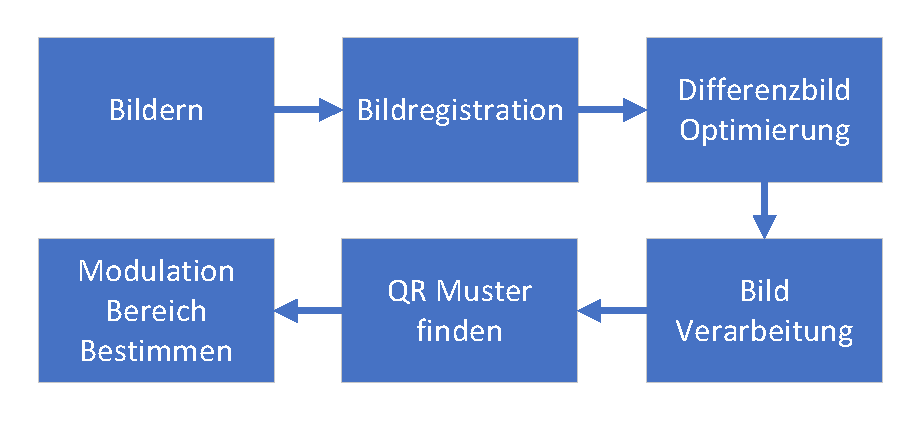
\includegraphics[keepaspectratio,width=1.0\textwidth]{images/3_Ersteverfahren/Strukturdiagramm.pdf}
 \caption{Strukturdiagramm}
 \label{fig:Strukturdiagramm}
\end{figure}

Das Objekt, das mit dieser Methode bearbeitet wird, ist eine aus einer spezifischen Smartphone App $ ``VLCReceiver" $ gesammelte Bilderreihe. Diese App wurde speziell für das \gls{david}-System entwickelt und erstellt eine Reihe von Bildern bei jeder Aufnahme. Im Allgemeinen wird die Kamera bei der Aufnahme in der Hand gehalten. Aufgrund von Handschütteln während der Aufnahme entsteht eine leichte Verschiebung zwischen den Bildern. Um dieses Problem zu beheben, wird eine Bildregistrierungsoperation verwendet, die zwei Bilder einer Aufnahme in dasselbe Koordinatensystem konvertiert. Zuerst werden durch \gls{surf} Merkmalserkennung Merkmale der Bilder verglichen. 
Durch Merkmalsextraktion und Merkmalsanpassung werden die Korrespondenzpunkte zwischen den verglichenen Bildern erhalten. Der \gls{ransac} Algorithmus benötigt, um die irrelevanten Korrespondentenpunkte zu beseitigen und die Genauigkeit zu verbessern. Aus dem Kameramodell wird anschließend ein mathematisches Transformationsmodell zwischen den entsprechenden Punkten in den beiden Bildern erstellt. Es ist zu beachten, dass der Prozess zur Lösung des Transformationsmodells als ein nichtlineares Optimierungsproblem angesehen werden kann. Durch die Lösung dieses Problems kann die Transformationsmatrix erhalten werden. In dieser Arbeit wird immer das erste Bild als Referenzbild gewählt um eine Bildregistrierung mit folgenden Bildern vorzunehmen. Die von der Bildregistrierung enthaltenen Bilder werden in dasselbe Koordinatensystem umgewandelt. Es werden je zwei Bilder subtrahiert, wodurch eine Reihe Differenzbilder entstehen. Um die folgende Detektion zu vereinfachen, wird eine Optimierungsoperation mit der Hilfe der geometrischen Eigenschaft des QR Musters unternommen woraufhin ein zu detektierendes Bild erstellt wird. Anschließend werden eine Reihe von Bildverarbeitungen bzw. Binarisierung, Medianfilter, Morphologie Operation vorgenommen. Dadurch können vereinzelt Punkte und Lücken, die durch Rauschen und Fehler verursacht wurden, entfernt werden. Schließlich wird es durch die Charakteristik des QR Musters, dessen Breiteverhältnis $1:1:3:1:1$ beträgt um QR Muster zu detektieren. Dies bestimmt auch den Modulationsbereich. Das Flussdiagramm wird in Abbildung \ref{fig:Flussdiagramm der Methode} gezeigt. Die Details jedes Teils werden in den folgenden Abschnitten beschrieben.

\begin{figure}[H]
 \centering 
 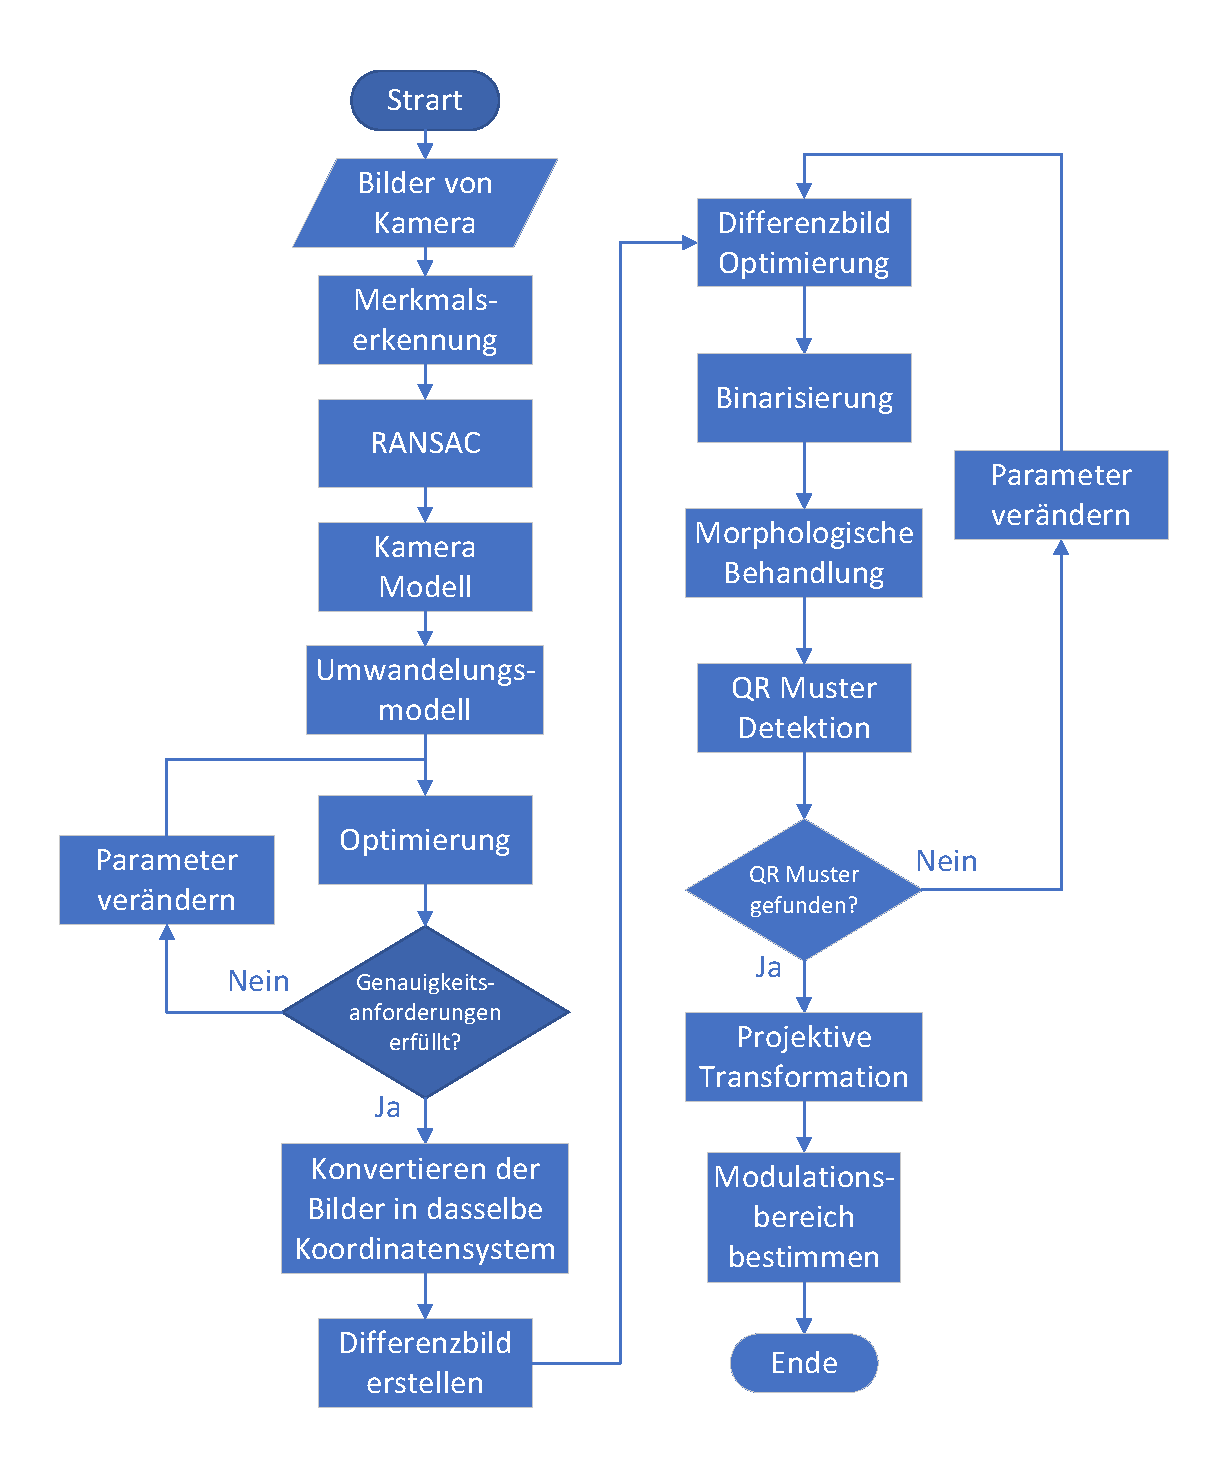
\includegraphics[keepaspectratio,width=1.0\textwidth]{images/3_Ersteverfahren/Flussdiagrammsum.pdf}
 \caption{Flussdiagramm der ersten Methode}
 \label{fig:Flussdiagramm der Methode}
\end{figure}

\section{Bildregistrierung} 

Es wird angenommen, eine Reihe Bilder wird mit einer Handheld-Kamera aufgenommen. Es kommt aufgrund von Handbewegungen zu einer leichten Verschiebung zwischen den beiden benachbarten Bildern. Wenn diese Bilder subtrahiert werden, um die Differenzbilder zu erhalten, wird das Ergebnis sehr schlecht sein. Um dieses Problem zu lösen, wird hier Bildregistrierung eingeführt. Ein Flussdiagramm der Bildregistrierung wird in Abbildung 4.2 gezeigt. 

\begin{figure}[H]
 \centering 
 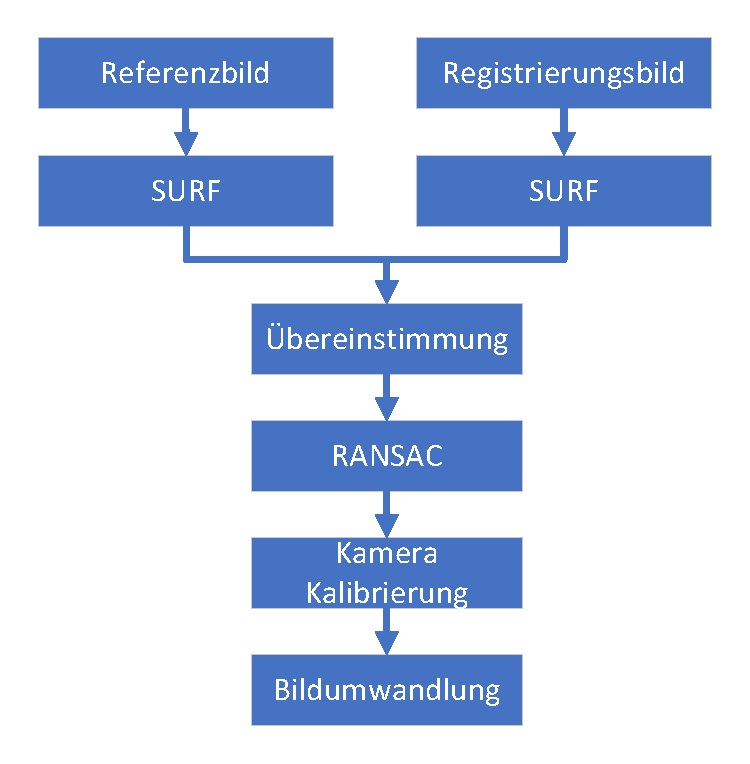
\includegraphics[keepaspectratio,width=0.6\textwidth]{images/3_Ersteverfahren/Bildregistration.pdf}
 \caption{Flussdiagramm der Bildregistrierung}
 \label{fig:Bildregistrierung}
\end{figure}

\subsection{\gls{surf}}
In jedem Bild gibt es eindeutige Pixelwertpunkte, d.h. Merkmalspunkte des Bildes. Um die Bilder in dasselbe Koordinatensystem zu transformieren, müssen diese Merkmalspunkte erkannt und analysiert werden. Deswegen ist es in diesem Verfahren besonders wichtig, die Merkmalspunkte eines Bildes zu definieren und zu finden. Um dieses Problem zu lösen, wird das Konzept der Merkmalserkennung eingeführt. Diese wird oft in Computer Vision und Bildverarbeitungsbereichen verwendet. Die Merkmalserkennung beinhaltet Verfahren zum Berechnen von Abstraktionen von Bildinformationen und zum Treffen lokaler Entscheidungen an jedem Bildpunkt, ob es an einem Punkt ein Bildmerkmal eines bestimmten Typs gibt oder nicht. Einige typische Merkmalserkennungen sind z.B. Kantenerkennung, Eckenerkennung, Tropfenerkennung und so weiter.

In dieser Arbeit wird das \gls{surf} \cite{Surf} genutzt. 
Dieser ist ein patentierter lokaler Merkmal-Detektor und Deskriptor und kann für Aufgaben wie Objekterkennung, Bildregistrierung, Klassifizierung oder 3D-Rekonstruktion angewandt werden. Diese Merkmalserkennung ist eine verbesserte Version von \gls{sift} Merkmalserkennung, die Haar-Wavelet verwendet um die Gradientenoperation in der \gls{sift}-Methode zu ersetzen, und gleichzeitig eine Integralgraph-Technik für schnelle Berechnungen verwendet. Die Faltung bezieht sich nur auf das vorherige Bild. Durch die Vergrößerung des Bildkerns kann das Heruntertaktungsverfahren realisiert werden. Die Geschwindigkeit von \gls{surf} ist 3-7 mal schneller als die von \gls{sift} welche in den meisten Fällen der Leistung von \gls{sift} entspricht. Daher wird \gls{surf} in vielen Anwendungen eingesetzt, insbesondere in Anwendungen in denen die Laufzeitanforderungen hoch sind. 

Der Verlauf einer \gls{surf} Merkmalserkennung ist wie folgend:

$\bullet$ \textbf{Aufbau einer hessischen Matrix.}\\
Die Hesse-Matrix stellt den Kern des \gls{surf} Algorithmus dar. Zur Vereinfachung der Operation wird für die Funktion $f(x,y)$ angenommen, dass sich die Hesse-Matrix H aus partiellen Ableitungen und Funktionen zusammensetzt.

\begin{equation}
   H(f(x,y)) = \begin{bmatrix}
   \frac{\partial^{2}f}{\partial x^{2}} & \frac{\partial^{2}f}{\partial x \cdot \partial y} \\
   \frac{\partial^{2}f}{\partial x \cdot \partial y} & \frac{\partial^{2}f}{\partial y^{2}} \\   
   \end{bmatrix}
\end{equation}

 Determinante der H-Matrix ist wie folgt:
 
\begin{equation}
   \det(H) = \frac{\partial^{2}f}{\partial x^{2}} \cdot \frac{\partial^{2}f}{\partial y^{2}} - (\frac{\partial^{2}f}{\partial x \cdot \partial y})^2  
\end{equation}

Der Wert der Determinante ist der Eigenwert der H-Matrix. Durch dessen positiven und negativen Wert wird bestimmt, ob der Punkt ein Extrempunkt ist oder nicht. Im \gls{surf} Algorithmus wird das Bildpixel $l(x,y)$ anstelle des Funktionswertes $f(x,y)$ verwendet. Es wird eine Gauß-Funktion zweiter Ordnung als Filter verwendet. Die zweiten partiellen Ableitungen können durch Faltung zwischen bestimmten Kernen berechnet werden. Dadurch können die Werte der drei Matrixelemente der H-Matrix ebenfalls berechnet werden.

\begin{equation}
\begin{split}
   &\mathcal{H}(\textbf{x},\sigma) = \begin{bmatrix}
   L_{xx}(\textbf{x},\sigma)\ L_{xy}(\textbf{x},\sigma) \\
   L_{xy}(\textbf{x},\sigma)\ L_{yy}(\textbf{x},\sigma)
   \end{bmatrix} \\   
   &L(\textbf{x},\sigma) = G(\sigma)*I(\textbf{x}) \\  
   &G(\sigma) = \frac{\partial^{2}g(\sigma)}{\partial x^{2}}      
\end{split}
\end{equation}


Hier bedeutet $L_{xx}(\textbf{x},\sigma)$ die Faltung der zweiten Gaußschen Ableitung $G(\sigma)$ mit dem Bild I im Punkt $\textbf{x}$(x,y), das selbe für $L_{xy}(\textbf{x},\sigma)$ und $L_{yy}(\textbf{x},\sigma)$. Auf diese Weise kann der Wert der Determinante für jedes Pixel in dem Bild berechnet werden und dieser Wert kann verwendet werden um den Merkmalspunkt festzustellen.
Zur einfacheren Anwendung schlägt Herbert Bay\cite{Surf} vor, L mit einer Approximation zu ersetzen. Um den Fehler zwischen dem genauen Wert und der Approximation auszugleichen, kann die H-Matrix-Determinante wie folgt ausgedrückt werden:

\begin{equation}
   \det(\mathcal{H}_{Approx}) = D_{xx}D_{yy} - (0.9D_{xy})^2  
\end{equation}
\\
$\bullet$ \textbf{Erstellen des Maßstabraums}\\
Der Maßstabraum $L(\textbf{x},\sigma)$ des Bildes ist die Darstellung dieses Bildes bei unterschiedlichen Auflösungen(Skalierungen). Im Bereich der Computer Vision wird der Maßstabraum symbolisch als Bildpyramide ausgedrückt, wobei die Eingangsbildfunktion wiederholt mit dem Kern der Gaußschen Funktion gefaltet und wiederholt unterabgetastet wird. Diese Methode wird hauptsächlich für die Implementierung des \gls{sift} Algorithmus verwendet. Jede Bildschicht hängt jedoch von der vorherigen Bildschicht ab, weshalb das Bild in der Größe angepasst werden muss. Daher büßt diese Berechnungsmethode viel Leistung ein. Das Gegenstück in \gls{surf} ist die Erhöhung der Größe des Bildkerns. Dies ist ein Unterschied zwischen dem \gls{sift} Algorithmus und dem \gls{surf} Algorithmus bei der Verwendung des Pyramidenprinzips.
Der Algorithmus ermöglicht, dass mehrere Bilder des Maßstabraums gleichzeitig verarbeitet werden, ohne dass das Bild unterabgetastet wird, wodurch die Leistung des Algorithmus verbessert wird. Das linke Bild in Abbildung \ref{fig:Scale space} ist eine Pyramidenstruktur, die auf herkömmliche Weise erstellt wird. Die Größe des Bildes wird geändert, und die Operation wird die Unterebene  unter Verwendung der Gaußschen Funktion wiederholt glätten. Der \gls{surf} Algorithmus auf der rechten Seite in Abbildung \ref{fig:Scale space} erhält das ursprüngliche Bild und ändert nur die Filtergröße.

\begin{figure}[htb]
 \centering 
 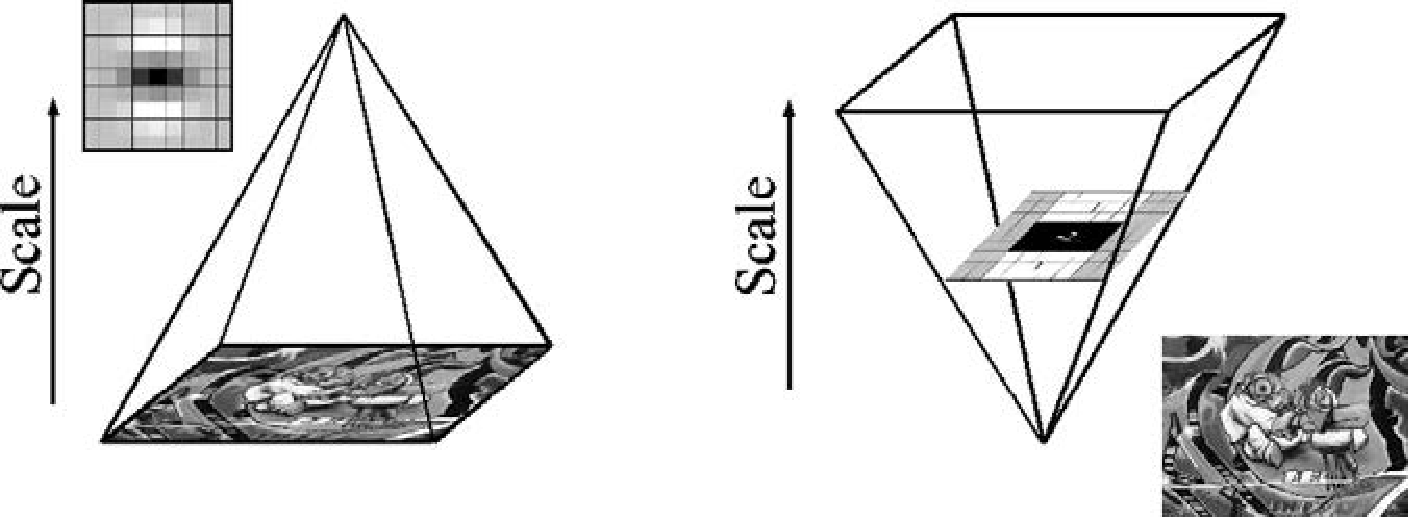
\includegraphics[keepaspectratio,width=0.8\textwidth]{images/3_Ersteverfahren/Scale_space.pdf}
 \caption{Scale space}
 \label{fig:Scale space}
\end{figure} 


$\bullet$ \textbf{Präzise Lokalisierung von Feature-Punkten}\\
Die von der Hesse-Matrix verarbeitete Größe jedes Pixels wird mit den 26 Punkten der drei Dimensionen im Raum, wie in Abbildung \ref{fig:Extremwert Erkennung} gezeigt, verglichen. Wenn einer davon das Maximum oder Minimum dieser 26 Punkte ist, wird dieser als vorläufiger Merkmalspunkt beibehalten. Das dreidimensionale lineare Interpolationsverfahren wird angewandt, um die Merkmalspunkte des Subpixel-Niveaus zu erhalten. Die Punkte, deren Werte kleiner als ein bestimmter Schwellenwert sind, werden ebenfalls entfernt.

\begin{figure}[htb]
 \centering 
 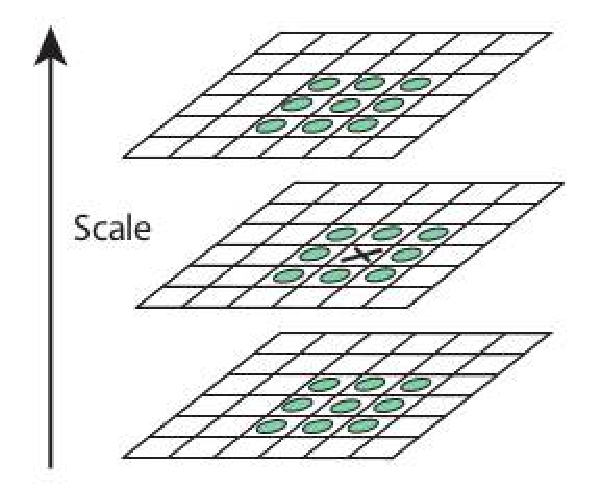
\includegraphics[keepaspectratio,width=0.4\textwidth]{images/3_Ersteverfahren/Extreme_Wert_Erkennung.pdf}
 \caption{Extremwert Erkennung}
 \label{fig:Extremwert Erkennung}
\end{figure} 


$\bullet$ \textbf{Hauptrichtungsermittlung}\\
\gls{sift} wählt die Hauptrichtung des Merkmalspunkts unter Verwendung des Gradientenhistogramms im Merkmalspunktbereich aus. Die Richtung, darin der Bin-Wert des Histogramms der größte ist oder 80\% des maximalen Bin-Werts überschreitet, wird als Hauptrichtung des Merkmalspunkts genommen. Dagegen beim \gls{surf}, wird nicht das Gradientenhistogramm, sondern die Haar-Wavelet-Eigenshcaft im Merkmalspunktbereich statistisch analysiert. Das heißt, im Bereich der Merkmalspunkte wird (zum Beispiel innerhalb eines Kreises mit einem Radius von 6\si{s}, wobei s der Maßstab ist auf dem der Punkt liegt), die Summe der Horizontal-Haar-Wavelet-Merkmale und der Vertikal-Haar-Wavelet-Merkmale aller Punkte im  60-Grad-Sektor($\pi/3$) gezählt. Die Größe des Haar-Wavelets beträgt 4\si{s}, sodass jeder Sektor einen Wert bekommt. Anschließend wird der 60-Grad-Sektor in einem bestimmten Intervall gedreht. Schließlich lässt die Richtung des Sektors anhand des Maximalwerts als Hauptrichtung vom Merkmalspunkt nehmen. Ein schematisches Diagramm des Prozesses ist wie folgt in Abbildung \ref{fig:Dominante Orientierung Feststellen}.

\begin{figure}[htb]
 \centering 
 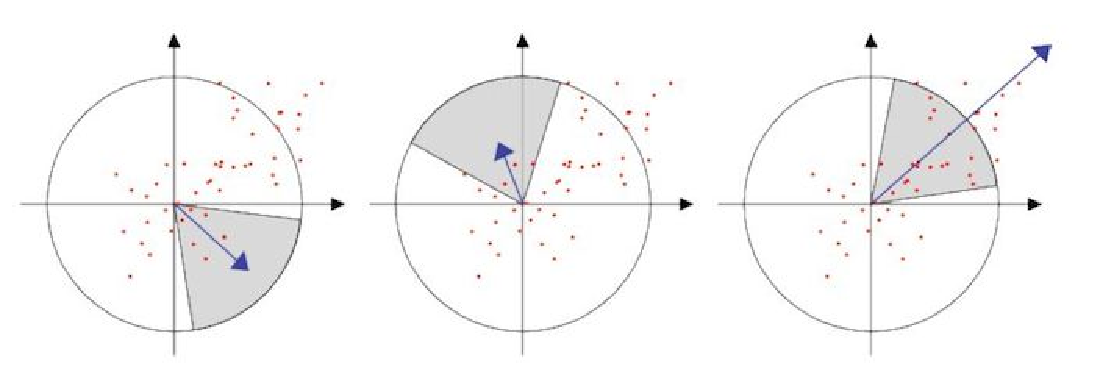
\includegraphics[keepaspectratio,width=0.8\textwidth]{images/3_Ersteverfahren/Dominante_Orientierung_Feststellen.pdf}
 \caption{Dominante Orientierung feststellen}
 \label{fig:Dominante Orientierung Feststellen}
\end{figure} 


$\bullet$ \textbf{Merkmalspunkt Deskriptor Generierung}\\
\gls{surf} generiert einen quadratischen Rahmen um den Merkmalspunkt. Die Größe der Seite des Rahmens ist 20\si{s} (s ist die Skala, dabei ein Merkmalspunkt erkannt wird). Die Richtung des Rahmens ist die Hauptrichtung, die im vorherigen Schritt erfasst wurde. Der Rahmen wird dann in 16 Unterbereiche unterteilt, von denen jeder die Haar-Wavelet-Merkmale der horizontalen und vertikalen Richtungen von 25 Pixeln berechnet. Hier sind die horizontalen und vertikalen Richtungen relativ zur Hauptrichtung. Das Haar-Wavelet-Merkmal ist die Summe der horizontalen Richtungswerte, die Summe der absoluten Werte in der horizontalen Richtung, die Summe der vertikalen Richtungen und die Summe der absoluten Werte in der vertikalen Richtung. Das schematische Diagramm in Abbildung \ref{fig:Merkmalspunkt Deskriptor} zeigt diesen Prozess.

\begin{figure}[htb]
 \centering 
 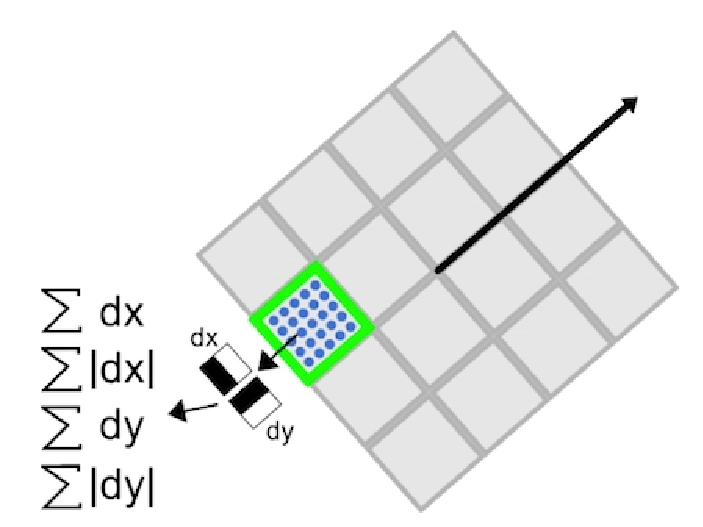
\includegraphics[keepaspectratio,width=0.5\textwidth]{images/3_Ersteverfahren/Merkmalspunkt_Deskriptor.pdf}
 \caption{Merkmalspunkt Deskriptor}
 \label{fig:Merkmalspunkt Deskriptor}
\end{figure} 

Auf diese Weise hat jeder kleine Bereich 4 Werte, so dass jeder Merkmalspunkt über einen $16*4=64$ dimensionalen Vektor verfügt, der nur halb so groß wie \gls{sift}(128 Dimension) ist, und deshalb den Anpassungsprozess beim Merkmalanpassungsprozess stark beschleunigt. Die folgende Abbildung \ref{fig:SURF Merkmal} zeigt die Merkmalspunkte, die durch den \gls{surf}-Algorithmus erhalten werden.

\begin{figure}[H]
 \centering 
 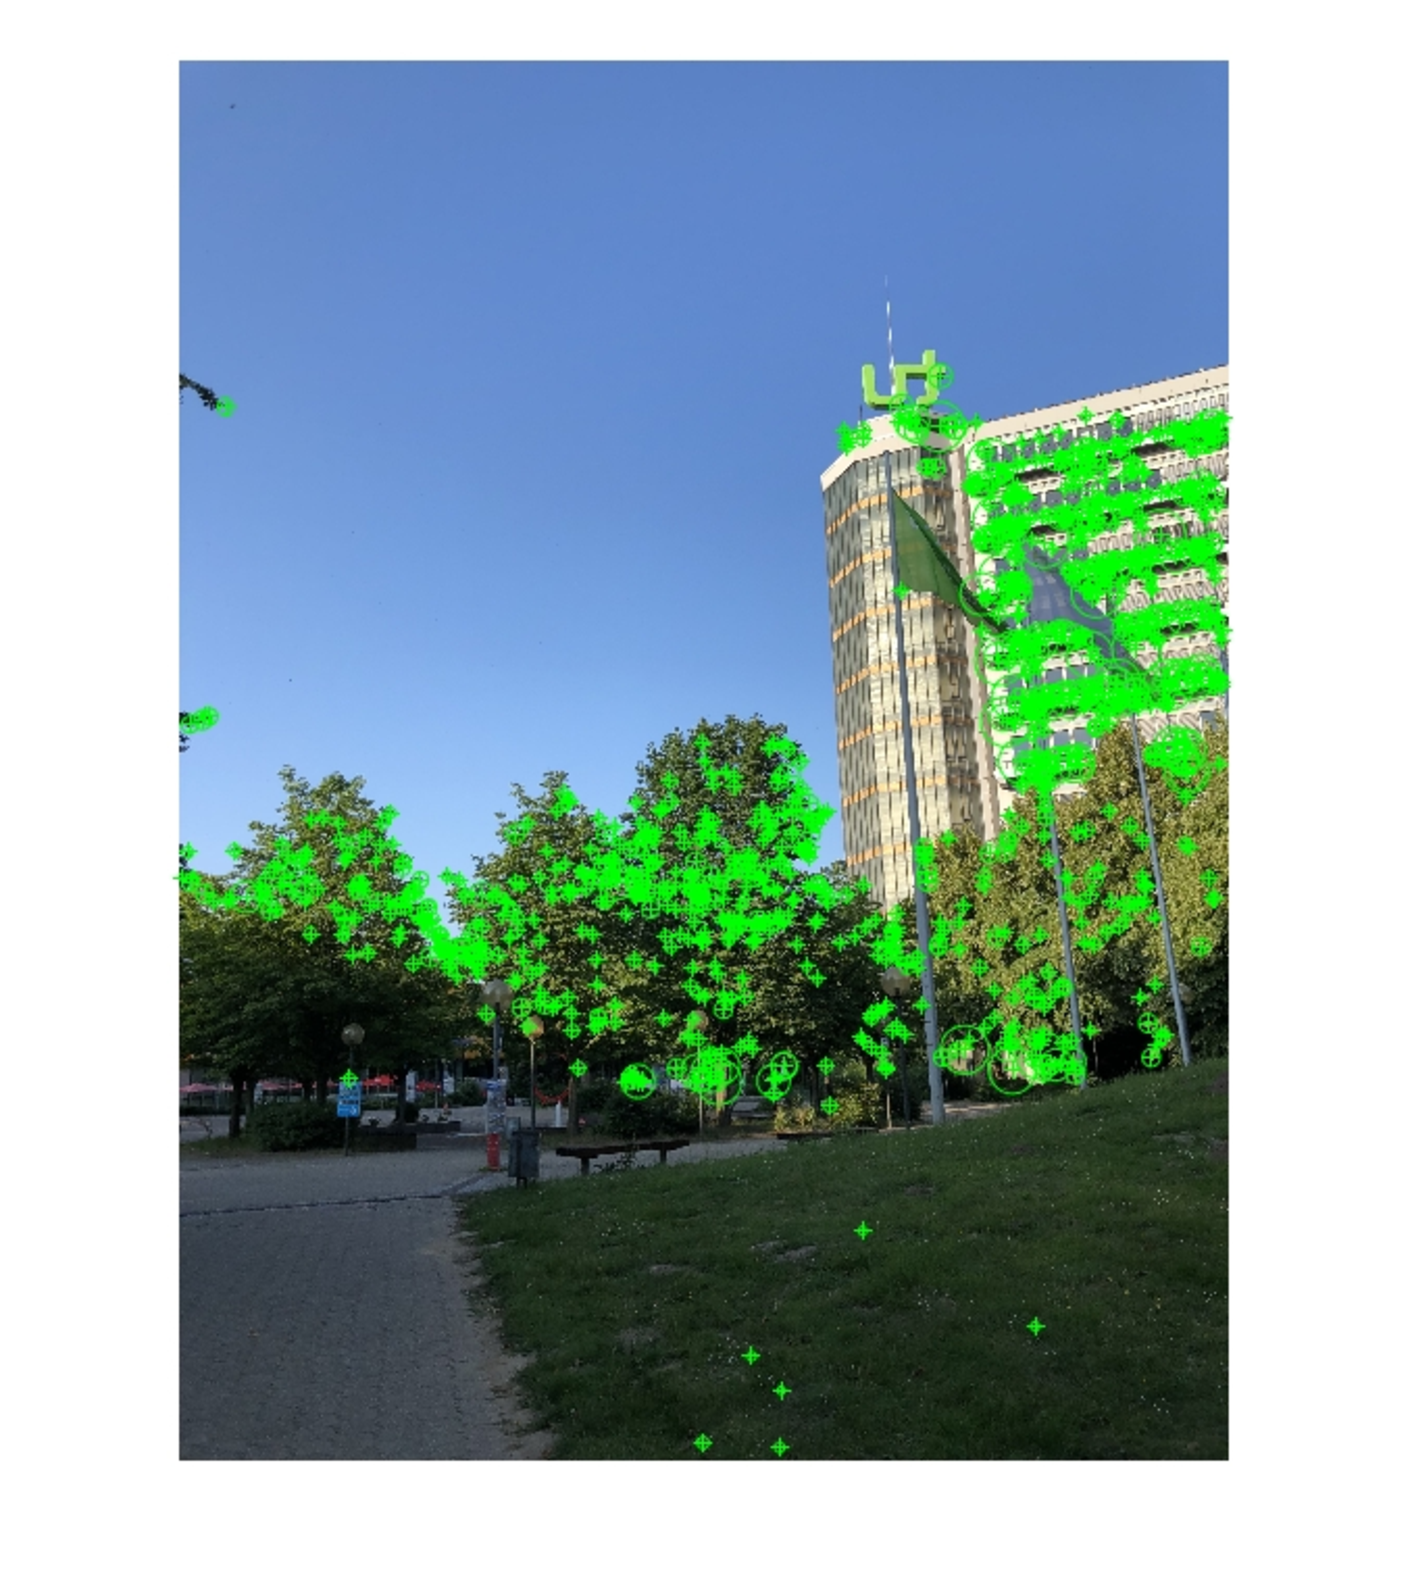
\includegraphics[keepaspectratio,width=0.8\textwidth]{images/3_Ersteverfahren/SURF_Detektion.pdf}
 \caption{\gls{surf} Merkmale}
 \label{fig:SURF Merkmal}
\end{figure} 


\subsection{\gls{ransac}}

Nach der \gls{surf} Merkmalserkennung werden die Merkmale von zwei benachbarten Bildern generiert. Diese Merkmale werden dann extrahiert und abgeglichen um entsprechende Punkte in den benachbarten zwei Bildern zu erhalten. Leider verbleiben durch diese Operation immernoch viele fehlerhafte zusammenpassende Paare. Deswegen wird hier \gls{ransac} verwendet, um die falschen Punkte zu beseitigen.

Der im Jahre 1981 vorgestellte \gls{ransac} Algorithmus von Fischler und Bolles \cite{ransac1}, ist ein allgemeiner Parameterschätzungsansatz um den großen Anteil von Ausreißern in den Eingabedaten zu bewältigen. Im Gegensatz zu vielen der üblichen robusten Schätzverfahren wie M-Schätzer und kleinste Quadrate, die von der Computer Vision Community aus der Statistik-Literatur übernommen wurden, wurde \gls{ransac} von der Computer-Vision-Community entwickelt. 

Ein einfaches Beispiel ist in der Abbildung \ref{fig:Linien Detektion} dargestellt. Das Ziel besteht darin, die am besten geeignete Linie unter einer Menge von Datenpunkten zu finden. Wenn es die einfache Methode der kleinsten Quadrate verwendet um diese Linie zu finden, wie auf der linken Seite gezeigt, kann es leider nicht richtig funktionieren, da die Methode der kleinsten Quadrate von allen Datenpunkten beeinflusst wird. Dagegen kann mit \gls{ransac} das Modell nur mit Potenziell korrekten Punkten berechnet werden, wie die Ergebnisse auf der rechten Seite zeigen. 

\begin{figure}[H]
 \centering 
 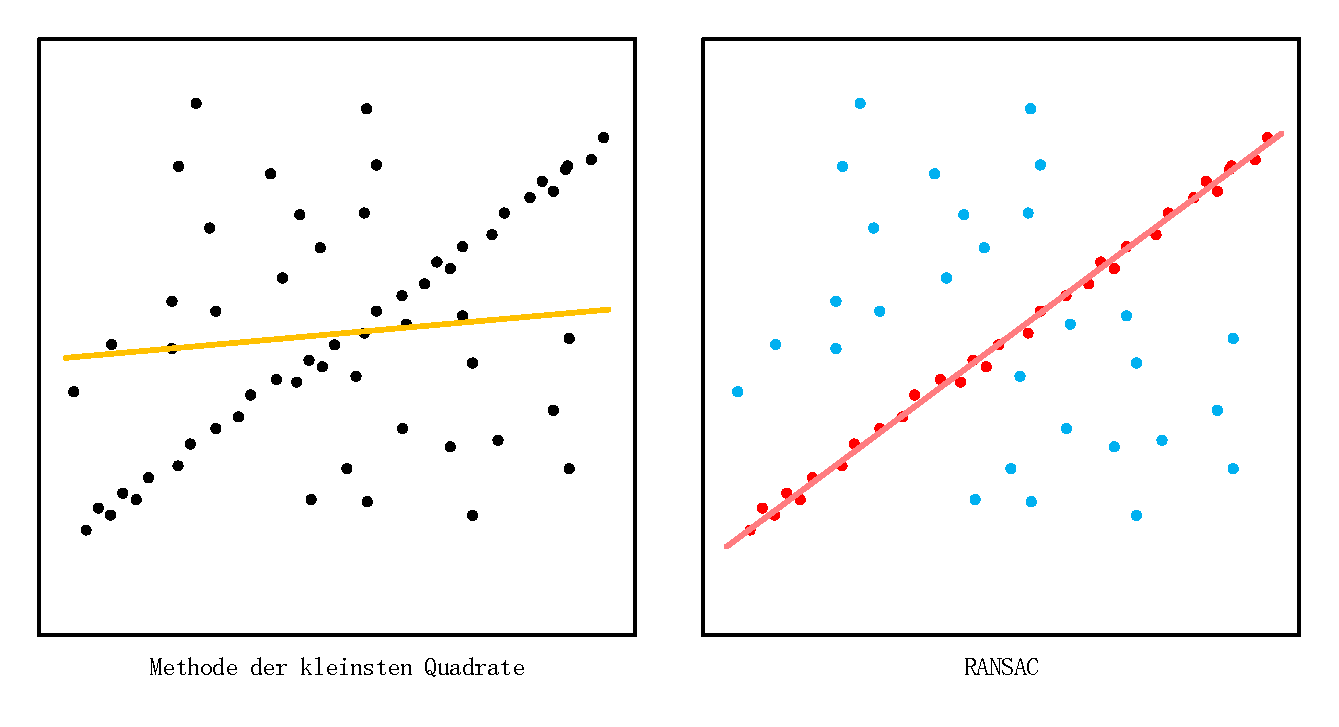
\includegraphics[keepaspectratio,width=1.0\textwidth]{images/3_Ersteverfahren/RANSAC/Linien_Detektion.pdf}
 \caption{Linien Detektion}
 \label{fig:Linien Detektion}
\end{figure} 

\gls{ransac} ist ein Wiederholungsprobennahme-Verfahren, welches durch die minimale Anzahl von Beobachtungenpunkten (Datenpunkten) die Kandidatenlösung generiert. Diese Datenpunkte sind erforderlich, um die zugrundeliegenden Modellparameter zu schätzen worauf Fischler und Bolles~\cite{ransac1} hingewiesen haben. Die Erhaltung einer anfänglichen Lösung und Ausschließung der Ausreißer mit dem \gls{ransac} Verfahren benötigt nicht so viele Daten, sondern verwendet die kleinste mögliche Menge und fährt fort, diese Menge mit konsistenten Datenpunkten zu vergrößern.

Der grundlegende Algorithmus ist wie folgt zusammengesetzt:

\begin{itemize}
	\item Zufällige Auswahl der Mindestanzahl erforderlicher Punkte zum Bestimmen der Modellparameter.
	\item Lösen der Parameter des Modells.
	\item Bestimmung der Punkte aus der Menge aller Punkte, welche mit einer vordefinierten Toleranz $\epsilon$ übereinstimmen
	\item Wenn ein Bruchteil der Anzahl von Inlierern über die Gesamtzahl der Punkte in dem Satz einen vordefinierten Schwellenwert $\tau$ überschreitet, schätzen die Modellparameter mit allen identifizierten Inlierern und terminieren.
	\item Ansonsten Wiederholung der Schritte 1 bis 4 (maximal N-mal).
\end{itemize}

N ist die Anzahl der Iterationen. Diese wird hoch genug gewählt, um die Wahrscheinlichkeit p (normalerweise 0.99) sicherzustellen, dass mindestens eine der Gruppen von Stichproben keinen Ausreißer enthält. Die Wahrscheinlichkeit, dass bei N mal iterieren mit erforderlich minimaler Anzahl von Punkten (hier m annahmen) mindestens ein Ausreißer mit ausgewählt wird, berechnet sich folgendermaßen:

\begin{equation}
   1 - p = (1 - u^m)^N
\end{equation}

u stellt die Wahrscheinlichkeit dar, dass jeder ausgewählte Datenpunkt ein Inlierer ist. Dagegen ist $v=1-u$ die Wahrscheinlichkeit, dass jeder ausgewählte Datenpunkt ein Ausreißer ist. Durch einige Gleichheitsumwandlungen kann die Anzahl der Iterationen ausgedrückt werden als:

\begin{equation}
   N = \frac{\log(1 - p)}{\log(1 - (1 - v)^m)}
\end{equation}

Abbildung \ref{fig:OhneRANSAC} zeigt die passenden Punkte durch Merkmalübereinstimmung mit der \gls{surf} Detektion. Es ist ersichtlich, dass es viele fehlerhafte Kombinationen gibt. Durch die Anwendung von \gls{ransac} kann dieses Problem effektiv gelöst und die übereinstimmenden Punkte verfeinert werden, wie das Ergebnis in Abbildung \ref{fig:MitRANSAC} zeigt.

\begin{figure}[H]
 \centering 
 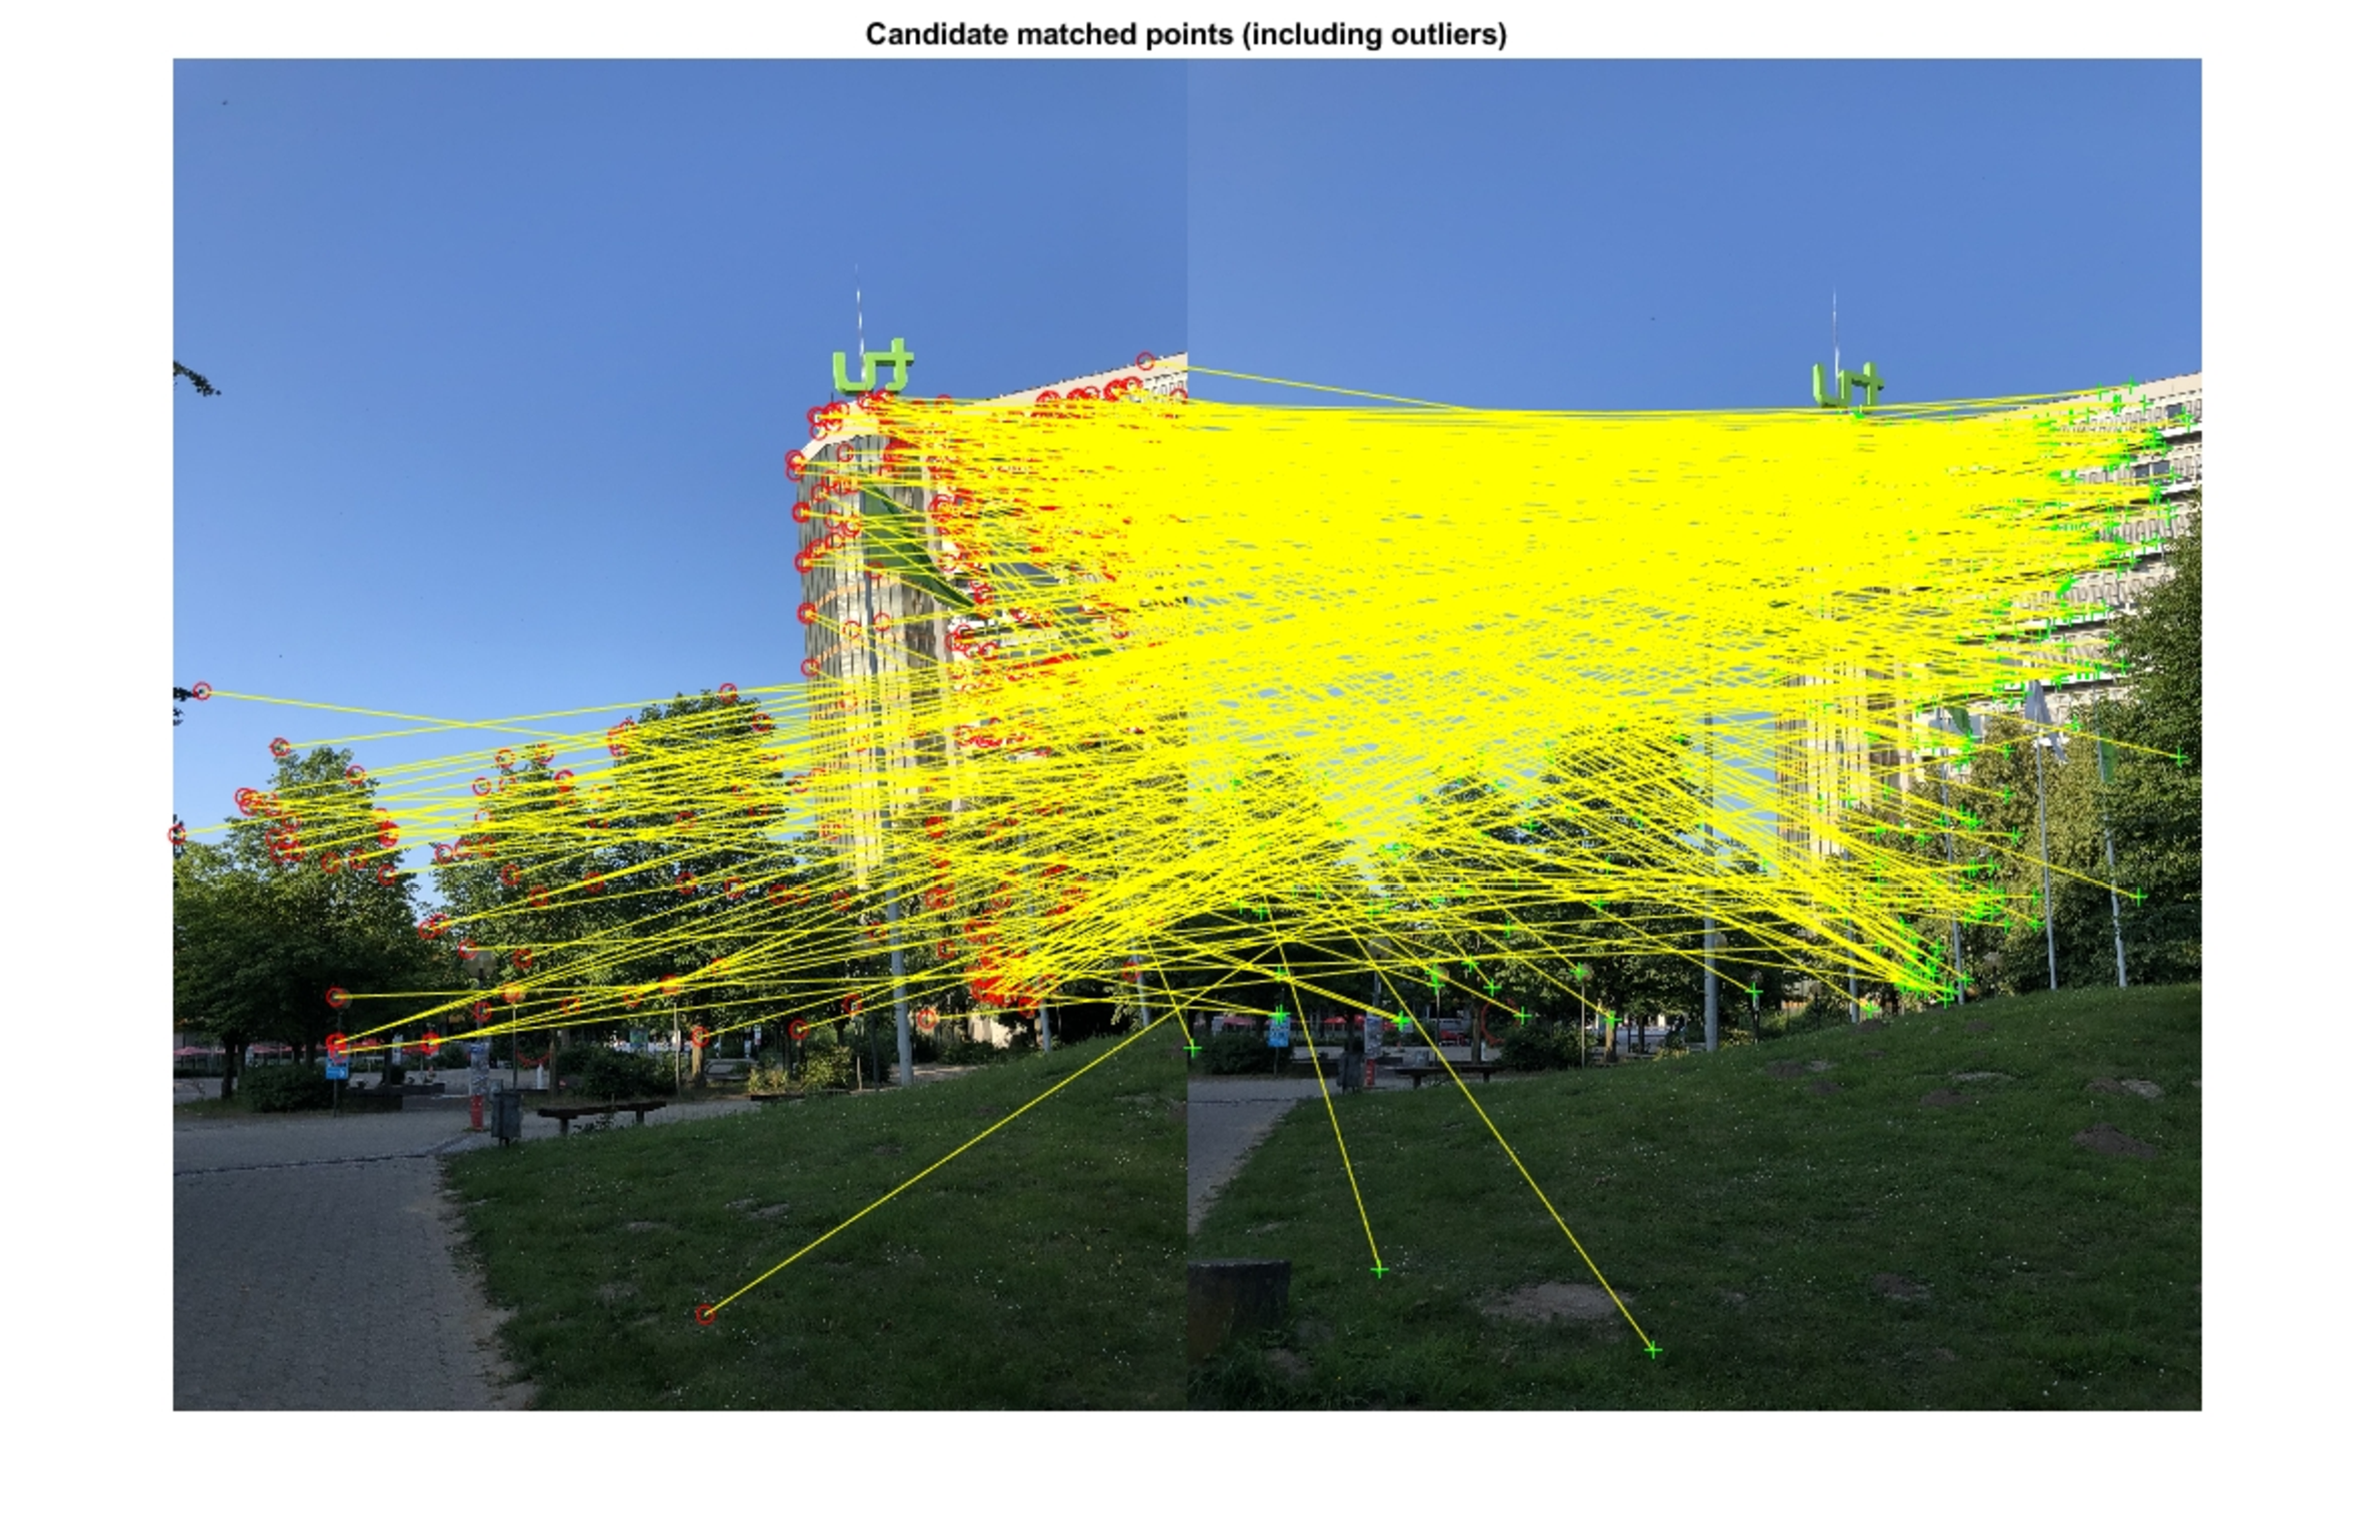
\includegraphics[keepaspectratio,width=0.9\textwidth]{images/3_Ersteverfahren/RANSAC/OhneRANSAC.pdf}
 \caption{Ohne \gls{ransac}}
 \label{fig:OhneRANSAC}
\end{figure} 

\begin{figure}[H]
 \centering 
 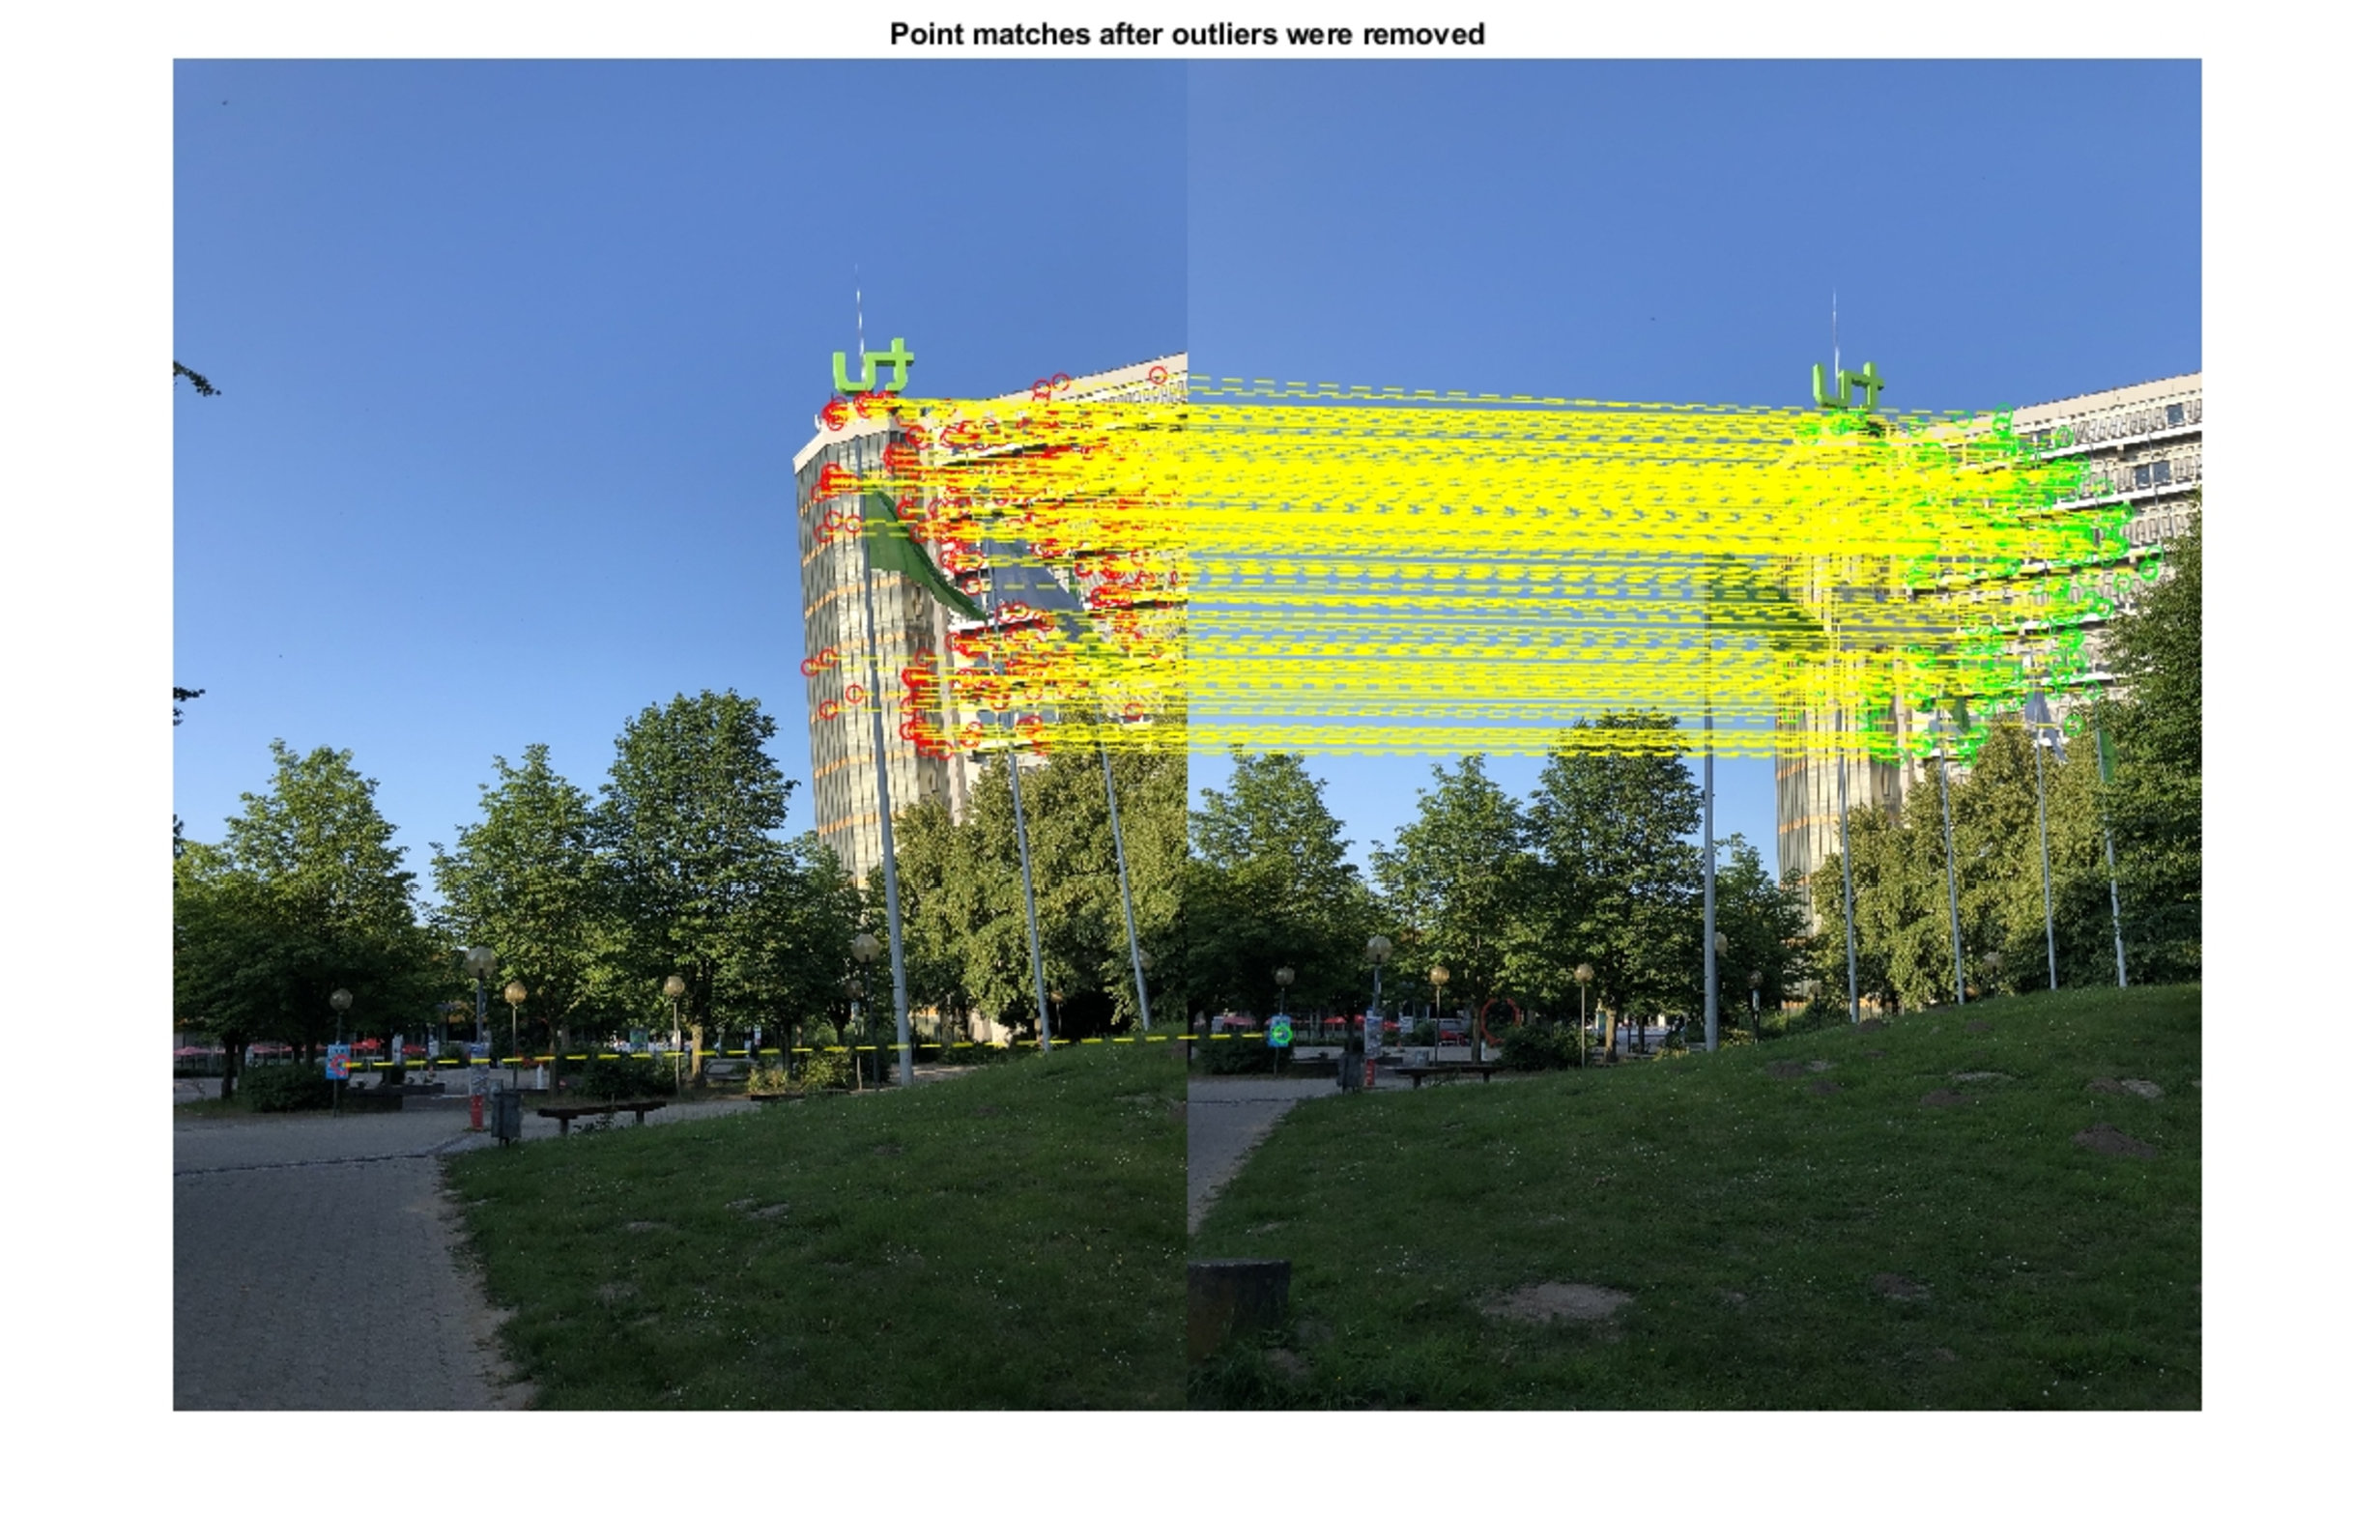
\includegraphics[keepaspectratio,width=0.9\textwidth]{images/3_Ersteverfahren/RANSAC/MitRANSAC.pdf}
 \caption{Mit \gls{ransac}}
 \label{fig:MitRANSAC}
\end{figure} 


\subsection{Bilder Umwandlung}

Wie in dem vorherigen Abschnitt vorgestellt, kann durch Verwenden des \gls{surf} übereinstimmende Punkte in aufeinanderfolgenden Bildern gefunden werden, anschließend lassen sich durch \gls{ransac} die Ausreißer ausschließen. Das Ziel dieses Abschnitts besteht darin, das Bild in dasselbe Koordinatensystem zu konvertieren. Der erste Schritt ist ein Kameramodell zu erstellen und anschließend die Umwandlungsbeziehung zwischen den entsprechenden Punkten in den zwei Bildern zu erhalten, um schließlich durch den Optimierungsalgorithmus die endgültige Transformationsmatrix zu erhalten. Die verschiedenen Schritte werden im Folgenden detailliert beschrieben.

\textbf{Kamera Modell}

Das Modell der Lochkamera ist in Abbildung \ref{fig:cameramodel} dargestellt. In dem Modell ist $O_C$ das optische Zentrum(Fokus) und f ist die Kamerabrennweite.

\begin{figure}[htb]
 \centering 
 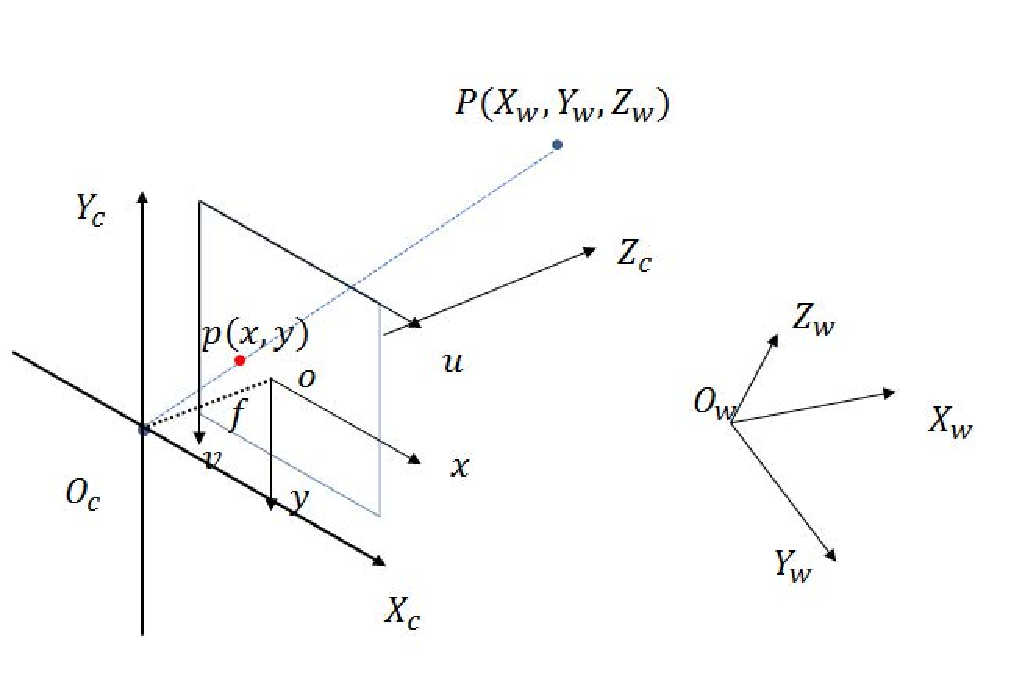
\includegraphics[keepaspectratio,width=0.8\textwidth]{images/3_Ersteverfahren/Kamera/cameramodel.pdf}
 \caption{Modell einer Lochkamera}
 \label{fig:cameramodel}
\end{figure} 

Die vier Koordinatensysteme im Modell sind wie folgt definiert:

\begin{itemize}
	\item 3D Weltkoordinatensystem $P(X_W,Y_W,Z_W)$ \\
	Punktkoordinaten werden durch homogene Koordinaten dargestellt: $\widetilde{X_w}\sim(X_W,Y_W,Z_W,1)^T$
	\item 3D Kamerakoordinatensystem $C(X_C,Y_C,Z_C)$\\
	Punktkoordinaten werden durch homogene Koordinaten dargestellt: $\widetilde{X_c}\sim(X_C,Y_C,Z_C,1)^T$
	\item 2D Bildabbildung Koordinatensystem $p(x,y)$\\
	Punktkoordinaten werden durch homogene Koordinaten dargestellt: $\widetilde{x}\sim(x,y,1)^T$
	\item 2D Bildpixel Koordinatensystem $I(u,v)$\\
	Punktkoordinaten werden durch homogene Koordinaten dargestellt: $\widetilde{u}\sim(u,v,1)^T$
\end{itemize}

% note
Unter diesem Modell wird ein 3D-Punkt im Weltkoordinatensystem durch drei Koordinaten den 2D-Bildpixelkoordinaten zugeordnet.

(\textbf{1}). 3D-Weltkoordinatensystem zum 3D-Kamera-Koordinatensystem.

Die Transformation vom Weltkoordinatensystem zum Kamerakoordinatensystem ist eine Starrekörpertransformation, d.h. das Objekt verformt sich nicht, sondern es rotiert nur und wird parallel verschoben. Diese Transformation wird in Abbildung \ref{fig:WzuC} gezeigt. R ist die Rotationsmatrix und T die Translationsmatrix.

\begin{figure}[htb]
 \centering 
 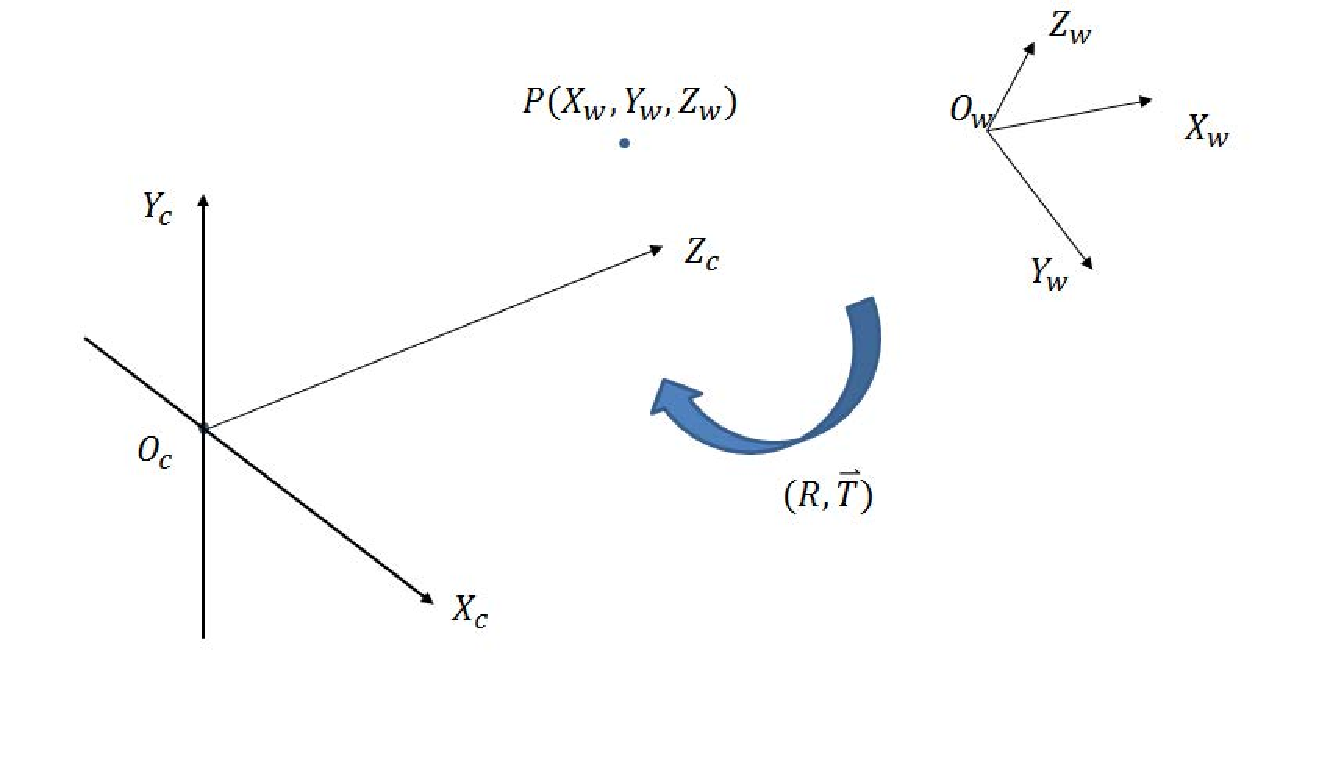
\includegraphics[keepaspectratio,width=0.8\textwidth]{images/3_Ersteverfahren/Kamera/WzuC.pdf}
 \caption{Transformation vom Weltkoordinatensystem zum Kamerakoordinatensystem}
 \label{fig:WzuC}
\end{figure} 

Um die entsprechende Rotationsmatrix zu erhalten, wird die Koordinatenachsen um verschiedene Winkel gedreht. Ein simples Beispiel wird in Abbildung \ref{fig:rotation} gezeigt.

\begin{figure}[H]
 \centering 
 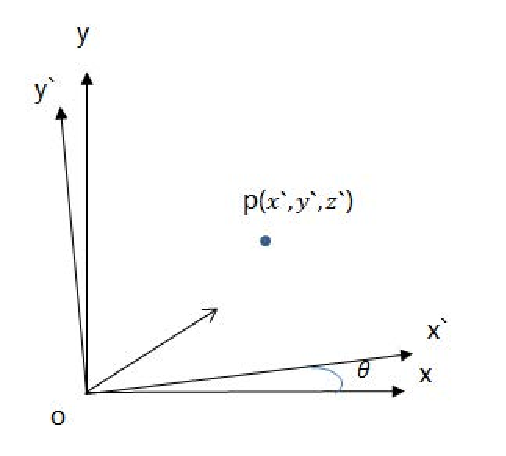
\includegraphics[keepaspectratio,width=0.4\textwidth]{images/3_Ersteverfahren/Kamera/rotationsmatrix.pdf}
 \caption{Rotation um Z-Achse}
 \label{fig:rotation}
\end{figure} 

Aus dem Bild kann leicht entnehmen werden:

\begin{equation}
   \begin{cases} 
	x = x'\cos\theta - y'\sin\theta \\	
	y = x'\sin\theta + y'\cos\theta \\
	z = z'
	\end{cases}
\end{equation}

In Matrixform wie folgt ausgedrückt:

\begin{equation}
   \begin{bmatrix}
	x \\  
	y \\
	z
	\end{bmatrix} = \begin{bmatrix}
	\cos\theta & -\sin\theta & 0	\\
	\sin\theta & \cos\theta  & 0	\\
	0    	   & 0           & 1	
	\end{bmatrix} \cdot \begin{bmatrix}
	x' \\  
	y' \\
	z'
	\end{bmatrix}= R_1 \cdot \begin{bmatrix}
	x' \\  
	y' \\
	z'
	\end{bmatrix}
\end{equation}

In ähnlicher Weise dreht sich die x-Achse, y-Achse um $\varphi$ und $\omega$ Grad wie folgt:

\begin{equation}
   \begin{bmatrix}
	x \\  
	y \\
	z
	\end{bmatrix} = \begin{bmatrix}
		1   & 0          & 0	\\
		0   & \cos\varphi & -\sin\varphi	\\
	    0   & \sin\varphi& \cos\varphi	
	\end{bmatrix} \cdot \begin{bmatrix}
	x' \\  
	y' \\
	z'
	\end{bmatrix}= R_2 \cdot \begin{bmatrix}
	x' \\  
	y' \\
	z'
	\end{bmatrix}
\end{equation}

\begin{equation}
   \begin{bmatrix}
	x \\  
	y \\
	z
	\end{bmatrix} = \begin{bmatrix}
	\cos\omega  & 0           & \sin\omega	\\		
	0    	    & 1           & 0	\\
	-\sin\omega &0            &  \cos\omega
	\end{bmatrix} \cdot \begin{bmatrix}
	x' \\  
	y' \\
	z'
	\end{bmatrix}= R_3 \cdot \begin{bmatrix}
	x' \\  
	y' \\
	z'
	\end{bmatrix}
\end{equation}

Schließlich kann die Rotationsmatrix erhalten werden:
\begin{equation}
   R = R_1 \cdot R_2 \cdot R_3
\end{equation}

Durch das Kombinieren der obigen Ergebnisse, lassen sich die Koordinaten von Punkt P im Kamerakoordinatensystem bestimmen:
\begin{equation}
   \begin{bmatrix}
	X_C \\  
	Y_c \\
	Z_c
	\end{bmatrix} = R \cdot \begin{bmatrix}
	X_w \\  
	Y_w \\
	Z_w 
	\end{bmatrix} +T
\end{equation}

Im homogenen Koordinatensystem dargestellt:
\begin{equation}
   \begin{bmatrix}
	X_C \\  
	Y_C \\
	Z_C \\
	1
	\end{bmatrix} = \begin{bmatrix}
	R & t	\\
	\vec{0}	& 1 \\
	\end{bmatrix} \cdot \begin{bmatrix}
	X_w \\  
	Y_w \\
	Z_w \\
	1
	\end{bmatrix}
\end{equation}

(\textbf{2}). 3D-Kamera-Koordinatensystem zum 2D-Bildabbildung Koordinatensystem.

Die Transformation vom Kamerakoordinatensystem zum Bildkoordinatensystem gehört zur perspektivischen Projektionsbeziehung von 3D zu 2D, wie in Abbildung \ref{fig:Czuimage} gezeigt.

\begin{figure}[H]
 \centering 
 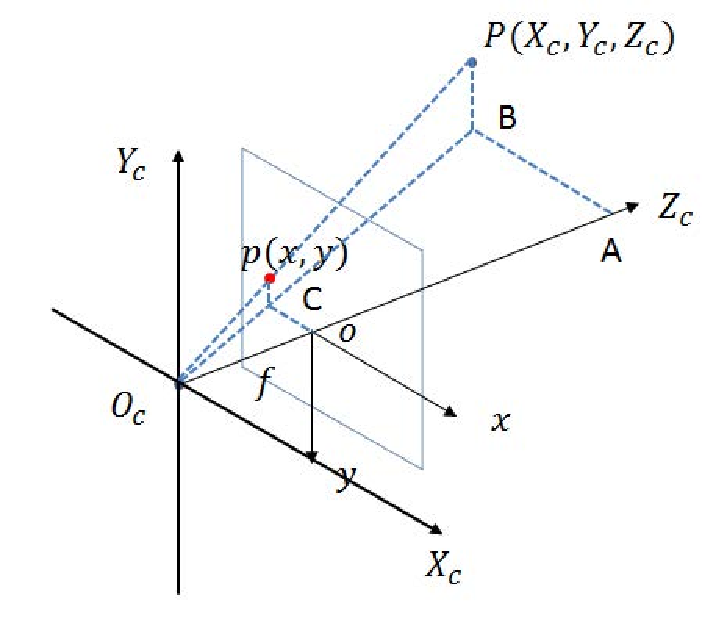
\includegraphics[keepaspectratio,width=0.4\textwidth]{images/3_Ersteverfahren/Kamera/Czuimage.pdf}
 \caption{Transformation vom Kamerakoordinatensystem zum Bildkoordinatensystem}
 \label{fig:Czuimage}
\end{figure} 

Es gibt zwei Paare mit ähnlichen Dreiecken:
\begin{equation}
   \begin{split}
    \triangle ABO_C \sim \triangle oCO_c\\  
	\triangle PBO_C \sim \triangle pCO_c
	\end{split}
\end{equation}

Aus ähnlichen Dreiecksbeziehungen kann diese Gleichung erstellt werden:
\begin{equation}
   \frac{AB}{oC} = \frac{AO_C}{oO_C} = \frac{PB}{pC} = \frac{X_C}{x} = \frac{Z_C}{f} = \frac{Y_C}{y} 
\end{equation}

Durch die Transformationsgleichung folgt: 
\begin{equation}
   x = f \cdot \frac{X_C}{Z_C}, y = f \cdot \frac{Y_C}{Z_C}
\end{equation}

Im homogenen Koordinatensystem dargestellt:
\begin{equation}
   Z_C \cdot \begin{bmatrix}
	x \\  
	y \\
	1
	\end{bmatrix} = \begin{bmatrix}
	f & 0 & 0 & 0	\\
	0 & f & 0 & 0	\\
	0 & 0 & 1 & 0	
	\end{bmatrix} \cdot \begin{bmatrix}
	X_C \\  
	Y_C \\
	Z_C \\
	1
	\end{bmatrix}
\end{equation}

Zu dieser Zeit ist die Einheit des Projektionspunkts p noch nicht Pixel, sondern Millimeter und muss weiter in das Pixelkoordinatensystem umgewandelt werden.

(\textbf{3}). 2D-Bildabbildung Koordinatensystem zum 2D-Bildpixel Koordinatensystem.

Das Pixelkoordinatensystem und das Bildkoordinatensystem befinden sich alle auf der Abbildungsebene, jedoch sind die jeweiligen Ursprünge und Maßeinheiten unterschiedlich. Der Ursprung des Bildkoordinatensystems ist der Schnittpunkt der optischen Achse der Kamera und der Abbildungsebene, üblicherweise der Mittelpunkt der Abbildungsebene oder der Hauptpunkt. Die Einheit des Bildkoordinatensystems ist Millimeter welche eine physikalische Einheit ist. Die Einheit des Pixelkoordinatensystems ist Pixel. Wie gewohnt wird beschrieben in welcher Zeile und Spalte ein Pixel ist. So ist der Übergang zwischen den beiden Koordinatensystem wie in Abbildung \ref{fig:Konvertierung von Pixelkoordinatensystem zu Bildkoordinatensystem} dargestellt. 

\begin{figure}[H]
 \centering 
 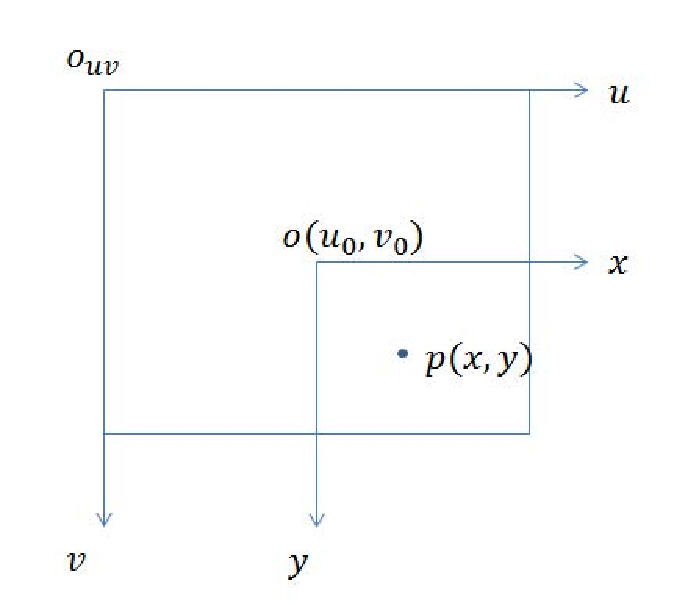
\includegraphics[keepaspectratio,width=0.5\textwidth]{images/3_Ersteverfahren/Kamera/imagezupixel.pdf}
 \caption{Konvertierung vom Bildkoordinatensystem zum Pixelkoordinatensystem}
 \label{fig:Konvertierung von Pixelkoordinatensystem zu Bildkoordinatensystem}
\end{figure} 

$d_x$ und $d_y$ ist die Größe jedes Pixel in den X- und Y-Achsenrichtungen. Jedes Pixel des Bildes hat die folgende Beziehung zwischen den zwei Koordinatensystemen.

\begin{equation}
   \begin{cases} 
	u = \frac{x}{d_x} + u_0	 \\  
	v = \frac{y}{d_y} + v_0	
	\end{cases}
\end{equation}

Im homogenen Koordinatensystem dargestellt:

\begin{equation}
   \begin{bmatrix}
	u \\  
	v \\
	1
	\end{bmatrix} = \begin{bmatrix}
	\frac{1}{d_x} 			& 0 			& u_0	\\
	0	 					& \frac{1}{d_y} & v_0	\\
	0     					& 0 			& 1	
	\end{bmatrix} \cdot \begin{bmatrix}
	x \\  
	y \\
	1
	\end{bmatrix}
\end{equation}

Es ist erwähnenswert, dass das Bildkoordinatensystem eine zweidimensionale Ebene(Bildebene), praktisch die Oberfläche des Kamera-CCD-Sensors ist. Jeder CCD-Sensor hat eine bestimmte Größe und Auflösung. Diese beiden Faktoren bestimmen die Konvertierungsbeziehung. Gegeben sei ein simples Beispiel: Eine Größe des CCD-Sensors ist $\SI{8}{\mm} \times \SI{6}{\mm}$, die Auflösung dafür ist $640~pixels \times 480~pixels$. Die Beziehung zwischen mm und Pixel ist $80~pixel/mm$. Ist die physikalische Größe jedes Pixels des CCD-Sensors $d_x \times d_y$, entspricht diese $d_x = d_y = \SI{1/80}{\mm}$.
 
Durch die Umwandlung der obigen vier Koordinatensysteme kann ein Punkt vom Weltkoordinatensystem zum Pixelkoordinatensystem extrahiert werden.
\begin{equation}
\begin{split}
   Z_C \cdot \begin{bmatrix}
	u \\  
	v \\
	1
	\end{bmatrix} & = \begin{bmatrix}
	\frac{1}{d_x} 			& 0 			& u_0	\\
	0	 					& \frac{1}{d_y} & v_0	\\
	0     					& 0 			& 1	
	\end{bmatrix} \cdot \begin{bmatrix}
	f & 0 & 0 & 0	\\
	0 & f & 0 & 0	\\
	0 & 0 & 1 & 0	
	\end{bmatrix} \cdot \begin{bmatrix}
	R & t	\\
	\vec{0}	& 1 \\
	\end{bmatrix} \cdot \begin{bmatrix}
	X_w \\  
	Y_w \\
	Z_w \\
	1
	\end{bmatrix} \\
	& = \begin{bmatrix}
	f_x & 0 & u_0 & 0	\\
	0 & f_y & v_0 & 0	\\
	0 & 0 & 1 & 0	
	\end{bmatrix} \cdot \begin{bmatrix}
	R & t	\\
	\vec{0}	& 1 \\
	\end{bmatrix} \cdot \begin{bmatrix}
	X_w \\  
	Y_w \\
	Z_w \\
	1
	\end{bmatrix}
\end{split}	
\end{equation}

Die erste Matrix der rechten Gleichung ist die allgemein bekannte interne Referenz der Kamera. Dagegen ist die zweite Matrix die externe Referenz der Kamera. Beide Parameter der Kamera können durch Zhang Zhengyou \cite{zhangzhengyou} Kalibrierung erhalten werden. Einige typische Kamera Parameter vom Werk aus sind der Tabellen \ref{tbl:Parameter der Kameras im Vergleich} zu entnehmen.

\begin{table}[htb]
	\captionabove{Parameter der Kameras im Vergleich}
	\label{tbl:Parameter der Kameras im Vergleich}
	\footnotesize
	\centering
	\rowcolors{2}{white}{gray!25}	%TUgreen!25
	\begin{tabular}{|p{3cm}|p{2.5cm}|p{2.5cm}|p{2.5cm}|}	%p{}m{}b{}clr
	\toprule
	\textbf{Parameter} & \textbf{Google Pixel} & \textbf{Google Pixel2} & \textbf{Iphone X}\\
	\midrule
	Sensor Größe $''$ & 1/2.3 & 1/2.6 & 1/3 \\
	Bild Auflösung $pixels$ & $4048 \times 3036$ & $4032 \times 3024$ & $4032 \times 3024$ \\
	Pixel Größe $\mu m$ & 1.544 & 1.4 & 1.22 \\	
	Brennweite $mm$ & 4.67 & 4.47 & 3.99 \\
	Formatfaktor $35 mm$  	&5.55	&6.04	&7.02	\\
	
	\bottomrule
	\end{tabular}
\end{table} 


Wenn die internen und externen Parameter der Kamera bekannt sind, ist es möglich daraus die Projektionsmatrix zu erstellen um daraus die Bildkoordinaten jeden beliebigen räumlichen Punkts zu erhalten. Wenn die Position $m(u,v)$ einer Bildkoordinate und die Parameter innerhalb und außerhalb der Kamera bekannt sind, kann der entsprechende Punkt in Weltkoordinate nur ungefähr bestimmt werden. Der Grund dafür ist, dass die $Z_c$ Information während des Projektionsprozesses eliminiert wird. 

\textbf{Umwandlungsmodelle}

Als nächstes wird die Umwandlungsbeziehung zwischen den entsprechenden Punkten in den beiden Bilder vorgenommen. Zuerst wird in dieser Arbeit eine vereinfachte Situation betrachtet, d.h. nur mit Rotationseinfluss. Abbildung \ref{fig:rotationsmodel} zeigt das 3D-Rotationsbewegungsmodell der Kamera. Die Position des optischen Zentrums ändert sich, während der Kamerabewegung im Drehbewegungsmodell der Kamera, nicht. Unter diesem Modell ist die Abbildungsbeziehung zwischen dem Punkt X im Weltkoordinatensystem und der Bildkoordinate x im homogenen Koordinatensystem dargestellt: 
\begin{equation}
   x = KRX, X = \lambda  K^{-1} x
\end{equation}

Wobei K der interne Parameter der Kamera ist, wie zuvor definiert. $\lambda$ ist der unbekannte Skalierungsfaktor, d.h. dass unter dem Kameramodell die Quelle jeder Bildpunktkoordinate einem Strahl zugeordnet ist.

\begin{figure}[H]
 \centering 
 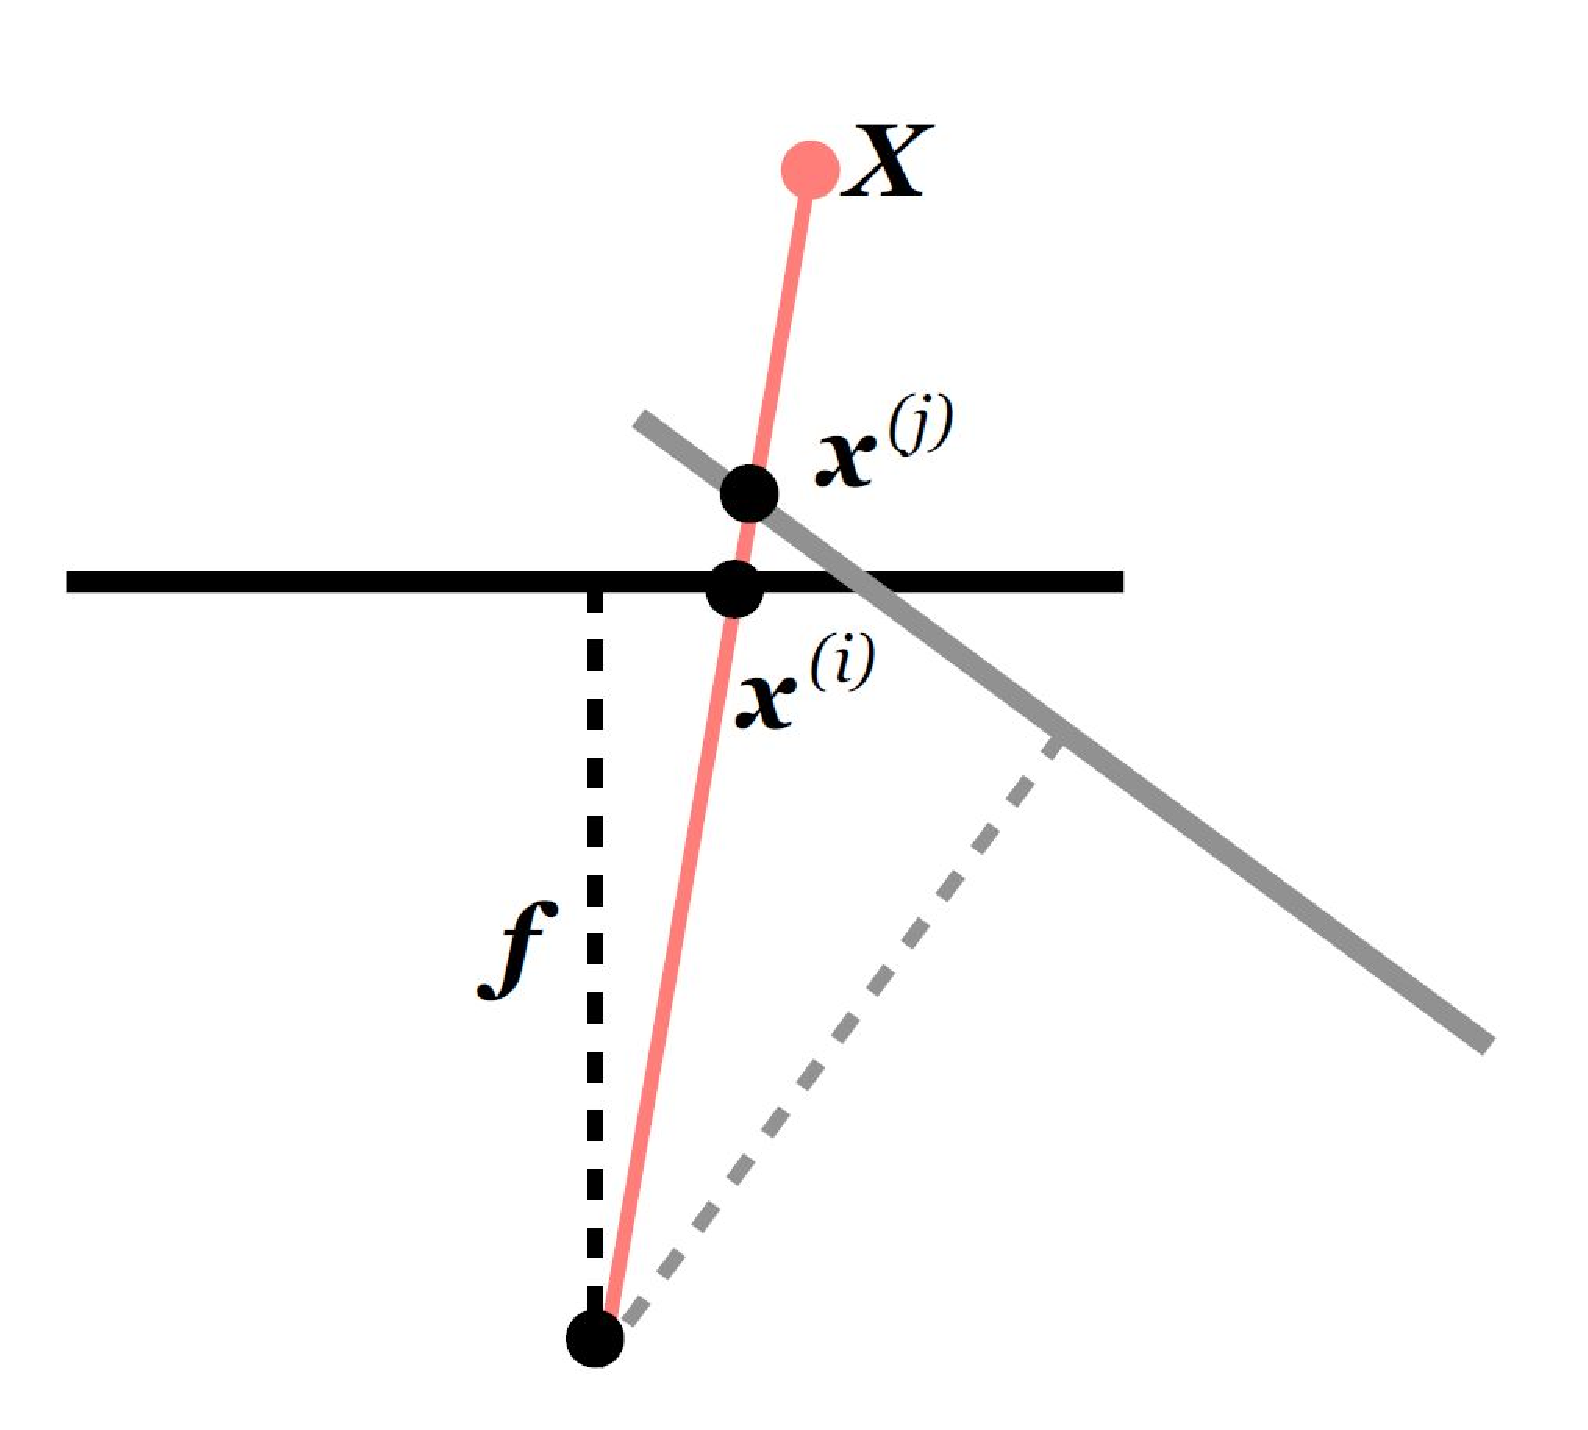
\includegraphics[keepaspectratio,width=0.5\textwidth]{images/3_Ersteverfahren/Kamera/rotationsmodel.pdf}
 \caption{Rotationsbewegungsmodell}
 \label{fig:rotationsmodel}
\end{figure} 

Nun wird die Beziehung zwischen Bildpunkten in einem Framepaar zwei verschiedener Kameraausrichtungen hergeleitet(siehe Abbildung \ref{fig:rotationsmodel}). Für einen Weltkoordinatepunkt X sind die projizierten Punkte $x_i$ und $x_j$ in der Bildebene von zwei Bildern i und j gegeben durch
\begin{equation}
   x_i = KR_iX, x_j = KR_jX
\end{equation}

Nach weiterem anordnen und ersetzen von X, wird eine Beziehung aller Punkte im Bildrahmen i auf alle Punkte im Rahmen j erhalten:
\begin{equation}
   x_j = KR_jR_i^TK^{-1}x_i
\end{equation}

Bisher wurde nur die Beziehung zwischen zwei Bildern der selben Aufnahme betrachtet. Diese Einschränkung wird gelockert, indem Frames von einer Kamera, die sich gemäß $R$ dreht, zu einer anderen Kamera, die sich gemäß $R'$ dreht, abgebildet werden. Es gibt eine Hypothese, dass beide Kamerazentren sich im Ursprung befinden. Mit der Warping-Matrix können die abgebildeten Punkte der Kameras wie folgt definiert werden:
\begin{equation}
   W = KR'R^TK^{-1}
\end{equation}

Hier wird das erste Bild als Referenzbild mit einem Rotationswinkel von 0 Grad gewählt, wodurch die Gleichung vereinfacht werden kann:
\begin{equation}
   W = KRK^{-1}
\end{equation}

Kombiniert mit Formel 3.23 kann es ausgedrückt werden als:
\begin{equation}
   x_j = Wx_i
\end{equation}

Diese Gleichung zeigt, dass jeder Punkt in dem Bild i nach der Transformationsmatrix W in einen entsprechenden Punkt in dem Bild j umgewandelt werden kann. Weiter in einem allgemeineren Fall, d.h. von nun an nicht nur mit Rotationseinfluss, sondern auch Translationseinfluss. Der Ableitungsverlauf ist im Allgemeinen gleich. Der Hauptunterschied ist die Anzahl der Parameter, die ursprünglich nur 3 Rotationsparameter aber jetzt 6 Parameter einschließlich 3 Rotationsparameter und 3 Translationsparameter beinhalten. Die neue Warping-Matrix sieht folgendermaßen aus:

\begin{equation}
   W = \begin{bmatrix}
	f			& 0 		& \frac{w}{2}	  & 0 \\
	0	 		& f			& \frac{h}{2} 	  & 0 \\
	0     		& 0 		& 1 			  & 0 \\	
	0     		& 0 		& 0 			  & 1
	\end{bmatrix} \cdot \begin{bmatrix}
	R_{11}			& R_{21}  		& R_{31}	  & 0 \\
	R_{12}	 		& R_{22}		& R_{32}	  & 0 \\
	R_{13}     		& R_{23} 		& R_{33} 	  & 0 \\	
	t1     			& t2 			& t3 		  & 1
	\end{bmatrix} \cdot \begin{bmatrix}
	\frac{1}{f}	   & 0 				& -\frac{w}{2f}	  & 0 \\
	0	 		   & \frac{1}{f}	& -\frac{h}{2f}   & 0 \\
	0     		   & 0 		        & 1 			  & 0 \\	
	0     		   & 0 		        & 0 			  & 1
	\end{bmatrix}
\end{equation}

\textbf{Transformationsoptimierung}

In den letzten beiden Abschnitten wurde die Transformationsmatrix zwischen den beiden Bildern aus dem Kameramodell abgeleitet. Hier in diesem Abschnitt werden die Parameter der Transformationsmatrix berechnet, also wird nun die Transformationsmatrix bestimmt. Hier sind die entsprechenden Punkte von zwei benachbarten Bildern $x_i, x_j$ bekannt und die Umwandlungsbeziehung dazwischen wird als die Formel 3.26 dargestellt. Angesichts dieser Bedingung 
kann die Berechnung der Transformationsmatrix als ein Optimierungsproblem betrachtet werden, wobei der Fehler J bei der Summenwertbildung im Quadrat aller Punktkorrespondenzen minimiert werden soll:

\begin{equation}
   J = \sum_{(i,j)}\lVert x_j - Wx_i \rVert ^2
\end{equation}

Zu Beachten ist, dass dies ein nichtlineares Optimierungsproblem ist. Einige nichtlineare Optimierer können ebenfalls verwendet werden um diese Zielfunktion zu minimieren. In der Kapital Evaluierung wurde bewissen, dass der Koordinatenabstieg durch direkte objektive Funktionsbewertung schnell konvergiert. Jedes Mal, wenn ein Schritt gemacht wird bei dem die Zielfunktion J nicht abnimmt, wird die Schrittrichtung umgekehrt und verringert die Schrittweite des entsprechenden Parameters. Der Algorithmus endet, sobald die Schrittgröße für alle Parameter unter einen gewünschten Schwellenwert fällt (d.h. Wenn die Zielgenauigkeit erreicht ist). 

Der detaillierte Algorithmus ist wie folgt dargestellt. Einige Definitionen werden hier eingeführt. $P_0$ ist der Vektor, der die Anfangswerte der Parameter speichert. Anschießend speichert er die Schrittgröße jedes Parameters in den Vektor $d_p$. $temp_dp$ ist der Vektor, in dem die gewünschten Schwellenwerte der Parameter gespeichert werden. D ist die Anzahl Unbekannter Parameter und W die Transformationsmatrix.

\textbf{1}. Zuerst durch Anfangswert $P_0$ Berechnung des anfänglichen Fehlers $J_0$.

\textbf{2}. Veränderung eines Parameters in eine entsprechende Schrittrichtung mit entsprechender Schrittgröße.

\textbf{3}. Berechnung der neuen Fehler $J_{new}$.

\textbf{4}. Vergleichen der beiden Fehler, ob der neue Fehler $J_{new}$ kleiner ist. Wenn Ja wird dieser neue Wert beibehalten. Wenn Nein wird die Schrittrichtung umgekehrt und die Schrittgröße auf ein Drittel des vorherigen Werts reduziert. Dann ändern das Objekt auf den nächsten Parameter und kehren zum zweiten Schritt zurück.

\textbf{5}. Wenn alle Schrittgrößen in $d_p$ den zuvor festgelegten Schwellenwert erreichen, wird der Algorithmus, mit Ausgabe des minimalen Fehlers J und der entsprechenden Transformationsmatrix, terminiert.

Das Flussdiagramm des Algorithmus ist wie in Abbildung \ref{fig:FlussdiagrammforOptimierung} dargestellt.

Durch die Transformationsmatrix können die Koordinaten des zweiten Bildes in die Koordinaten des ersten Bildes übertragen werden. Abbildung \ref{fig:Transformation in eine Koordinate} zeigt diesen Verlauf. Schließlich kann durch Subtraktion das Differenzbild erzeugt werden.

\begin{figure}[H]
 \centering 
 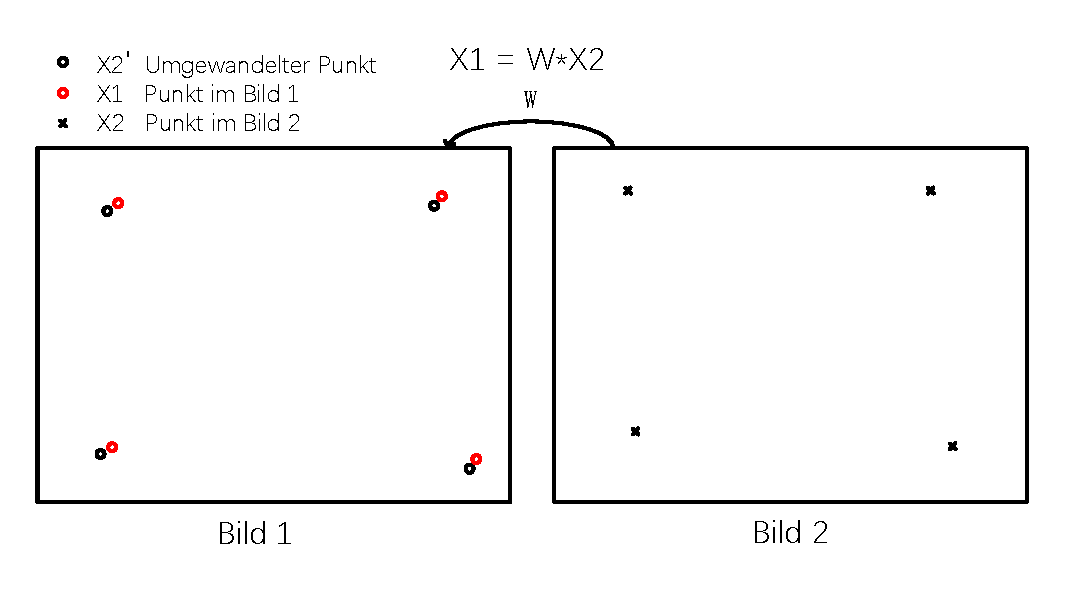
\includegraphics[keepaspectratio,width=0.8\textwidth]{images/3_Ersteverfahren/Kamera/Transformmatrix.pdf}
 \caption{Transformation in das selbe Koordinatensystem}
 \label{fig:Transformation in eine Koordinate}
\end{figure} 

\begin{figure}[H]
 \centering 
 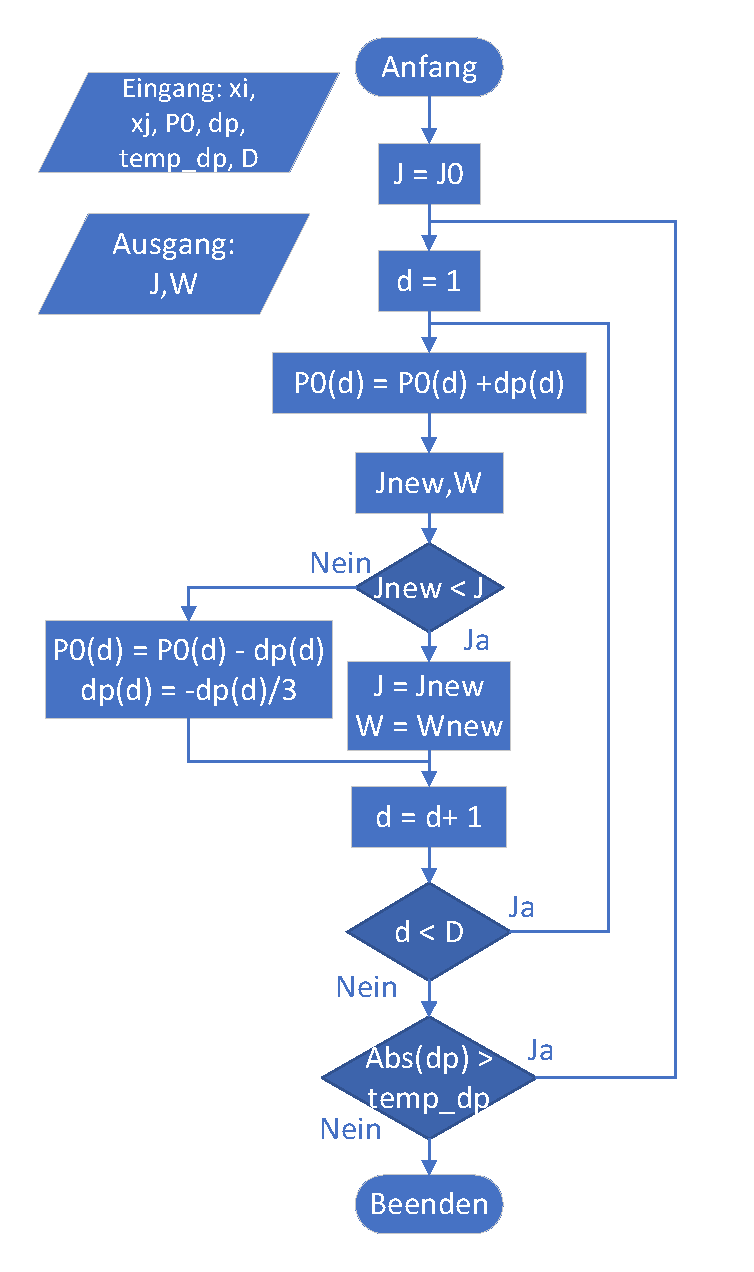
\includegraphics[keepaspectratio,width=0.8\textwidth]{images/3_Ersteverfahren/Kamera/flussdiagramm_for_parameter.pdf}
 \caption{Flussdiagramm für Optimierung}
 \label{fig:FlussdiagrammforOptimierung}
\end{figure} 



\section{Differenzbild Optimierung}
Die Bildregistration liefert eine Reihe Bilder von der Kamera, deren Koordinaten in dasselbe Koordinatensystem umgewandelt wurden. Es werden je zwei Bilder ausgewählt und subtrahiert, um eine Reihe Differenzbilder zu erhalten. Das Ziel in diesem Abschnitt ist, von diesen Differenzbildern ein zu detektierendes Bild herzustellen, das die QR Muster Detektion vereinfacht. Es sollte hier beachtet werden, dass aufgrund der Zeitsynchronisation die QR Muster in den Differenzbildern einige unerwartete Effekte aufweisen könnten. Eine mögliche Formel der Differenzbilder wie folgt mit der Anhahme dass es in vertikaler Richtung ist.

\begin{itemize}
	\item total Schwarz-Weiß-Schwarz-Weiß-Schwarz Ordnung.
	\item halb Schwarz-Weiß-Schwarz-Weiß-Schwarz Ordnung, halb nicht gezeigt.
	\item total Weiß-Schwarz-Weiß-Schwarz-Weiß Ordnung.
	\item halb Weiß-Schwarz-Weiß-Schwarz-Weiß Ordnung, halb nicht gezeigt.
	\item halb Schwarz-Weiß-Schwarz-Weiß-Schwarz Ordnung, halb Weiß-Schwarz-Weiß-Schwarz-Weiß Ordnung.
	\item total nicht gezeigt.
\end{itemize}

Tabelle \ref{tbl:differenzbildformel} zeigt solche Situationen und listet auf, ob sie zur folgenden Detektion angepasst sind. Die direkte Verwendung dieser Differenzbilder ist für die nächste Detektion ein kniffliges Problem. Um dieses Problem zu lösen, wurde ein Algorithmus zur Optimierung der Differenzbilder entwickelt.

\begin{table}[htb]
	\captionabove{mögliche Differenzbilder}
	\label{tbl:differenzbildformel}
	\footnotesize
	\centering
	\rowcolors{2}{white}{gray!25}	%TUgreen!25
	\begin{tabular}{|p{2cm}<{\centering}|c|p{2cm}<{\centering}|c|}	%p{}m{}b{}clr p{3cm} p{8cm}
	\toprule
	\textbf{Ob angepasst zu folgender Detektion?} & \multirow{4}{*}{\textbf{Differenzbild}} & \textbf{Ob angepasst zu folgender Detektion?} & \multirow{4}{*}{\textbf{Differenzbild}} \\
	\midrule
	 Ja & 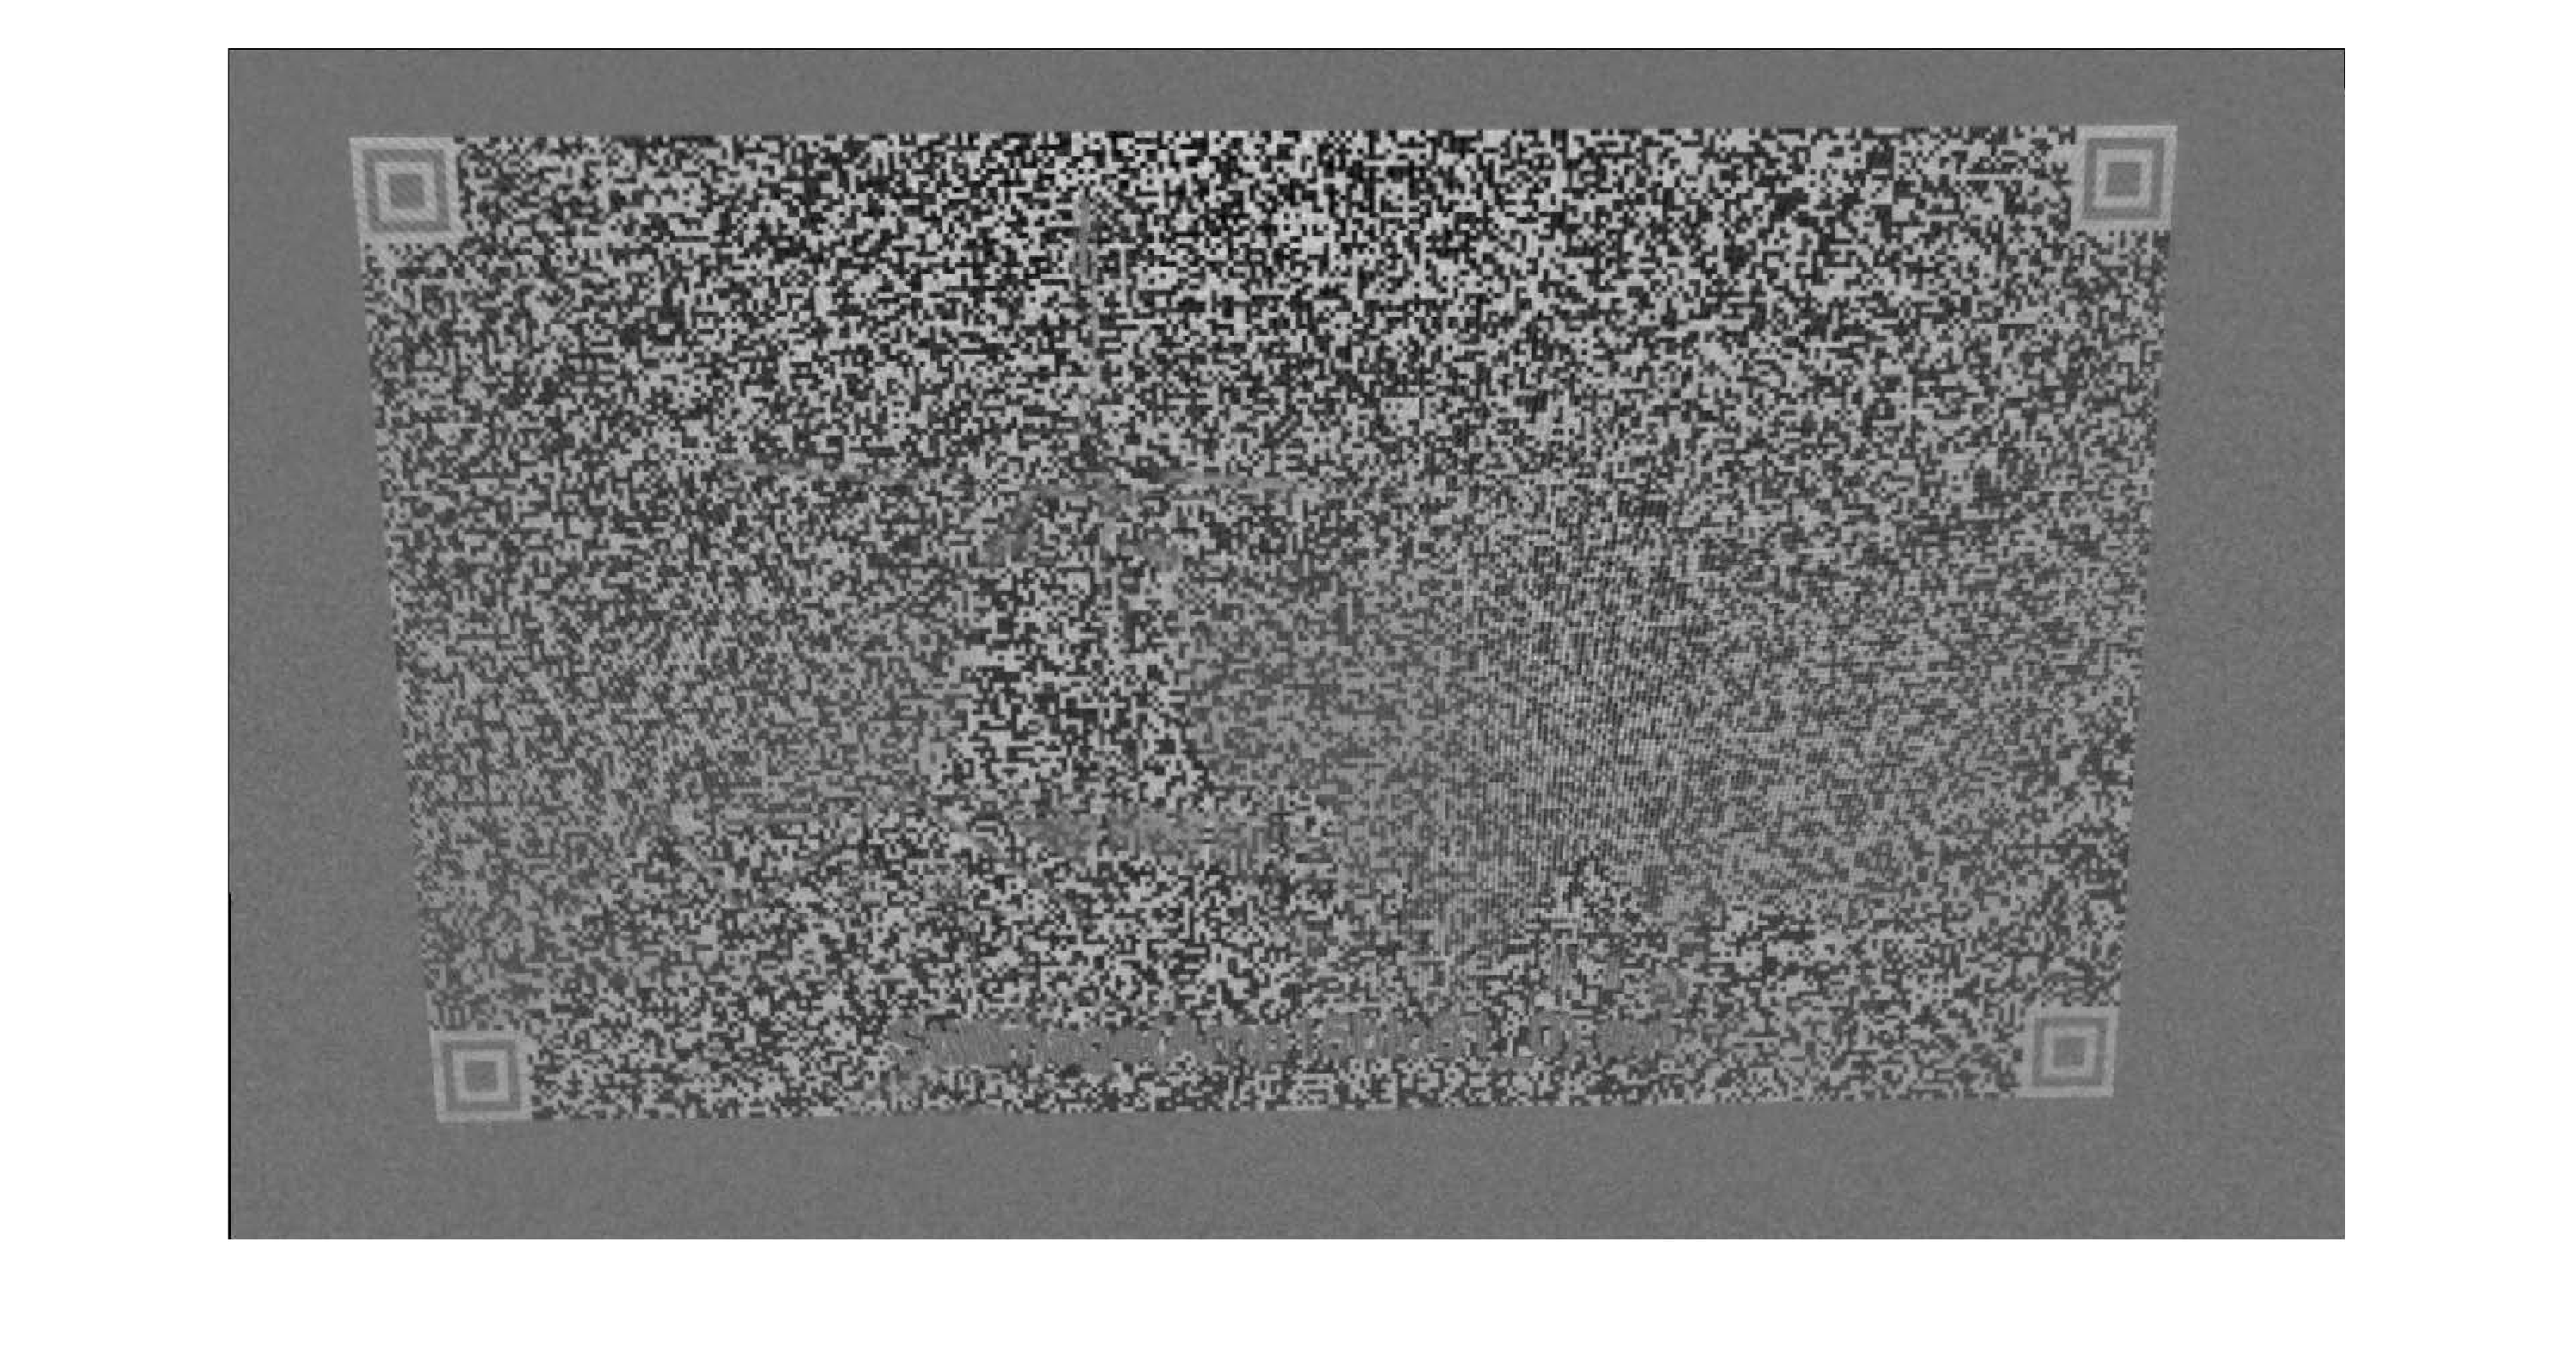
\includegraphics[scale=0.12]{images/3_Ersteverfahren/Differenzbild/0schwarz.pdf}& Nein & 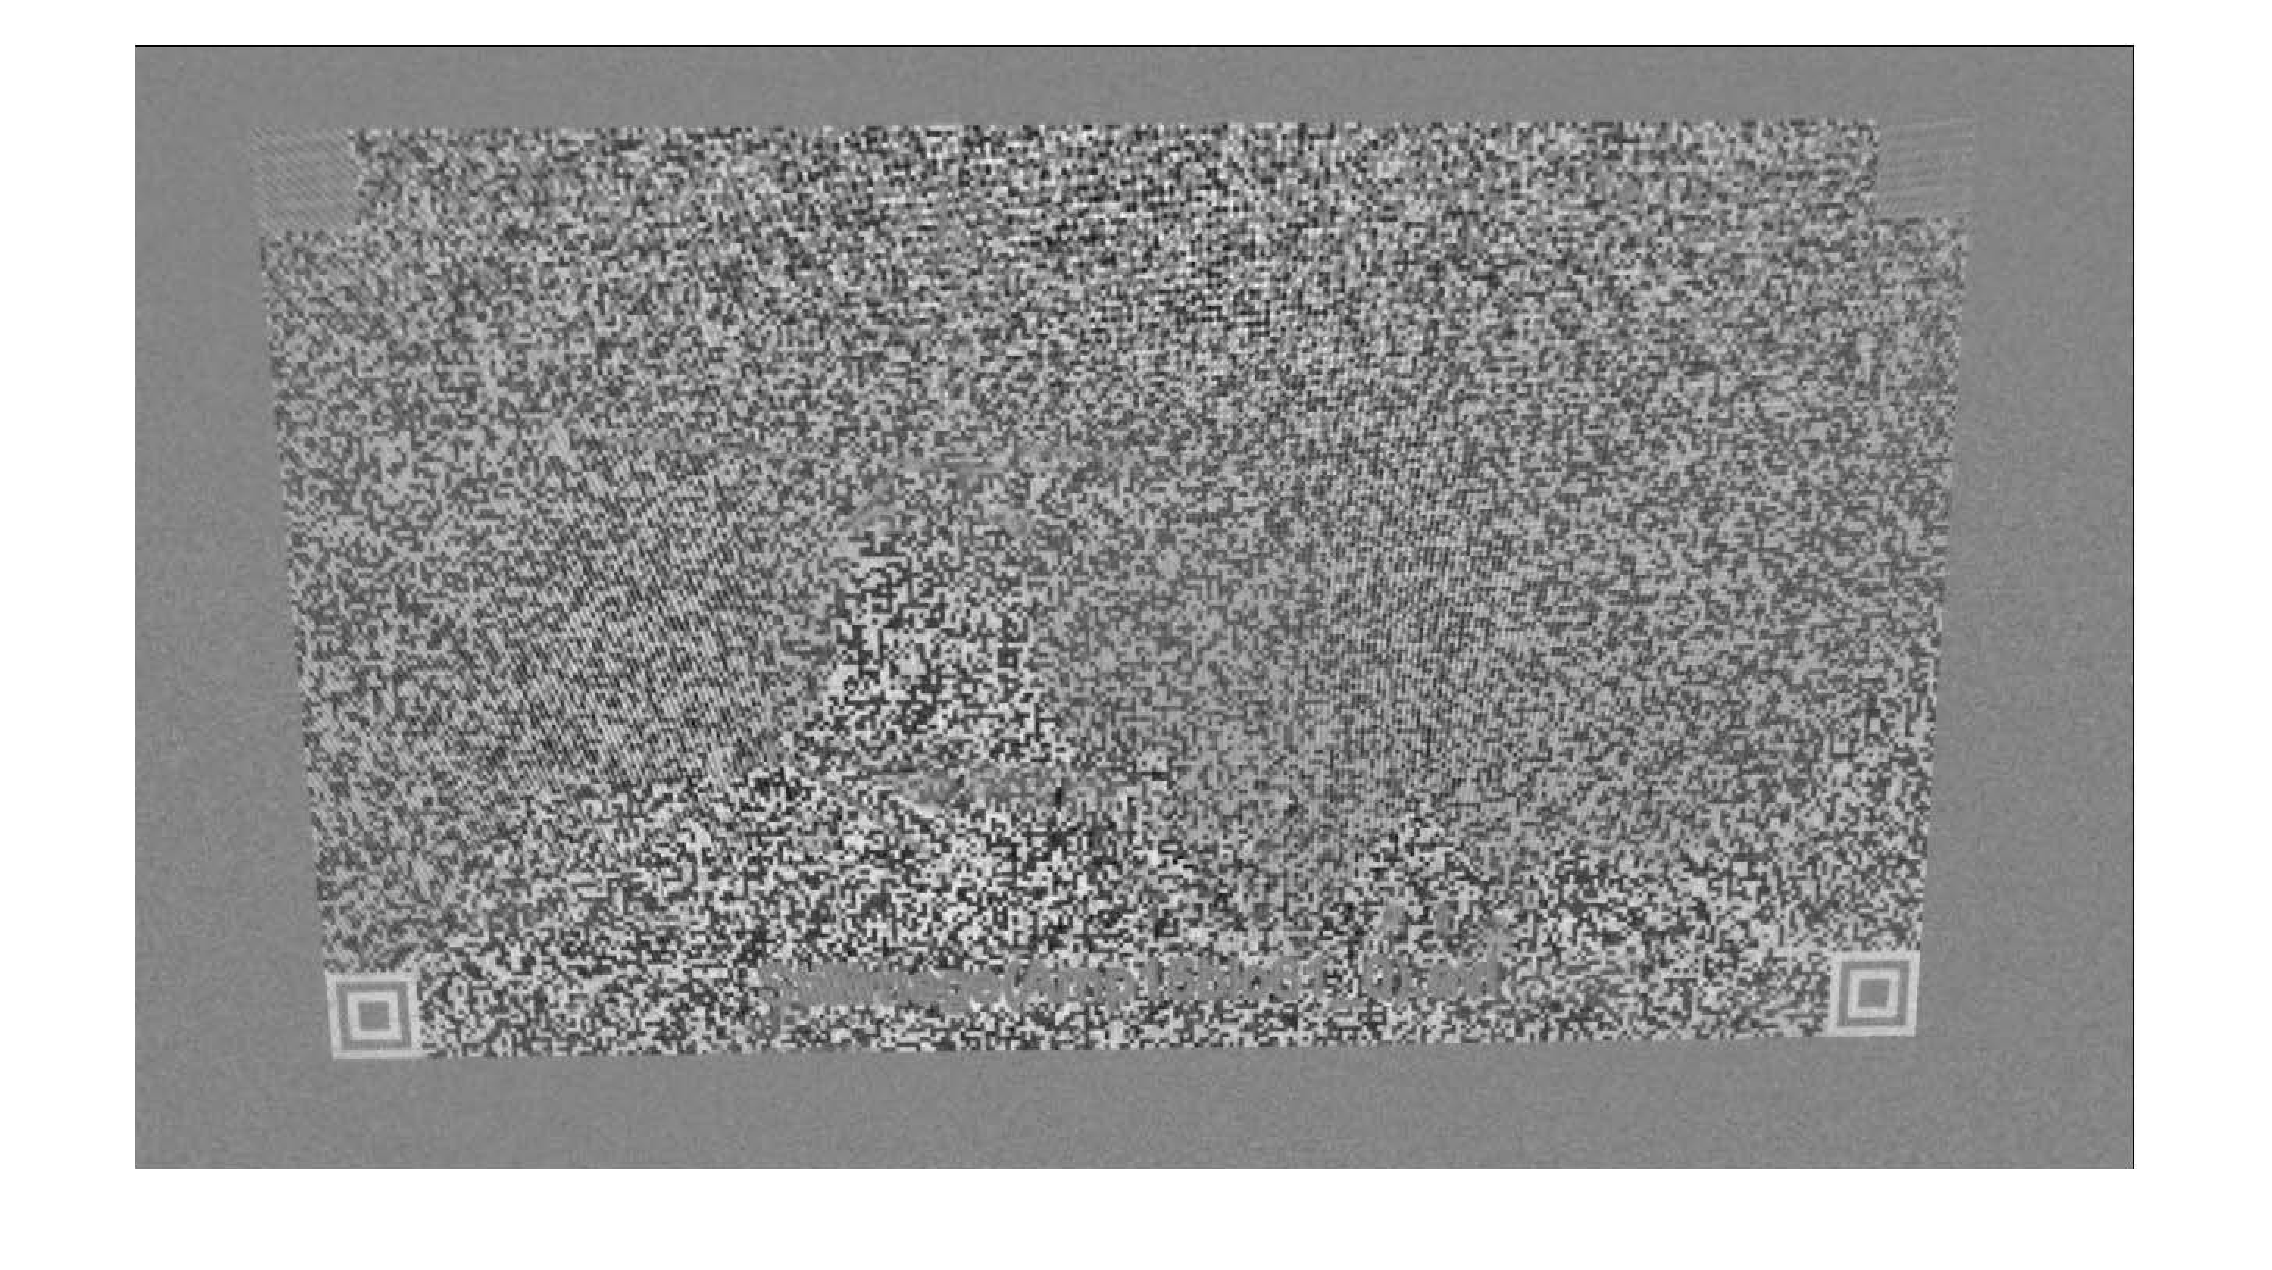
\includegraphics[scale=0.15]{images/3_Ersteverfahren/Differenzbild/1halfschwarz.pdf}\\
	Nein & 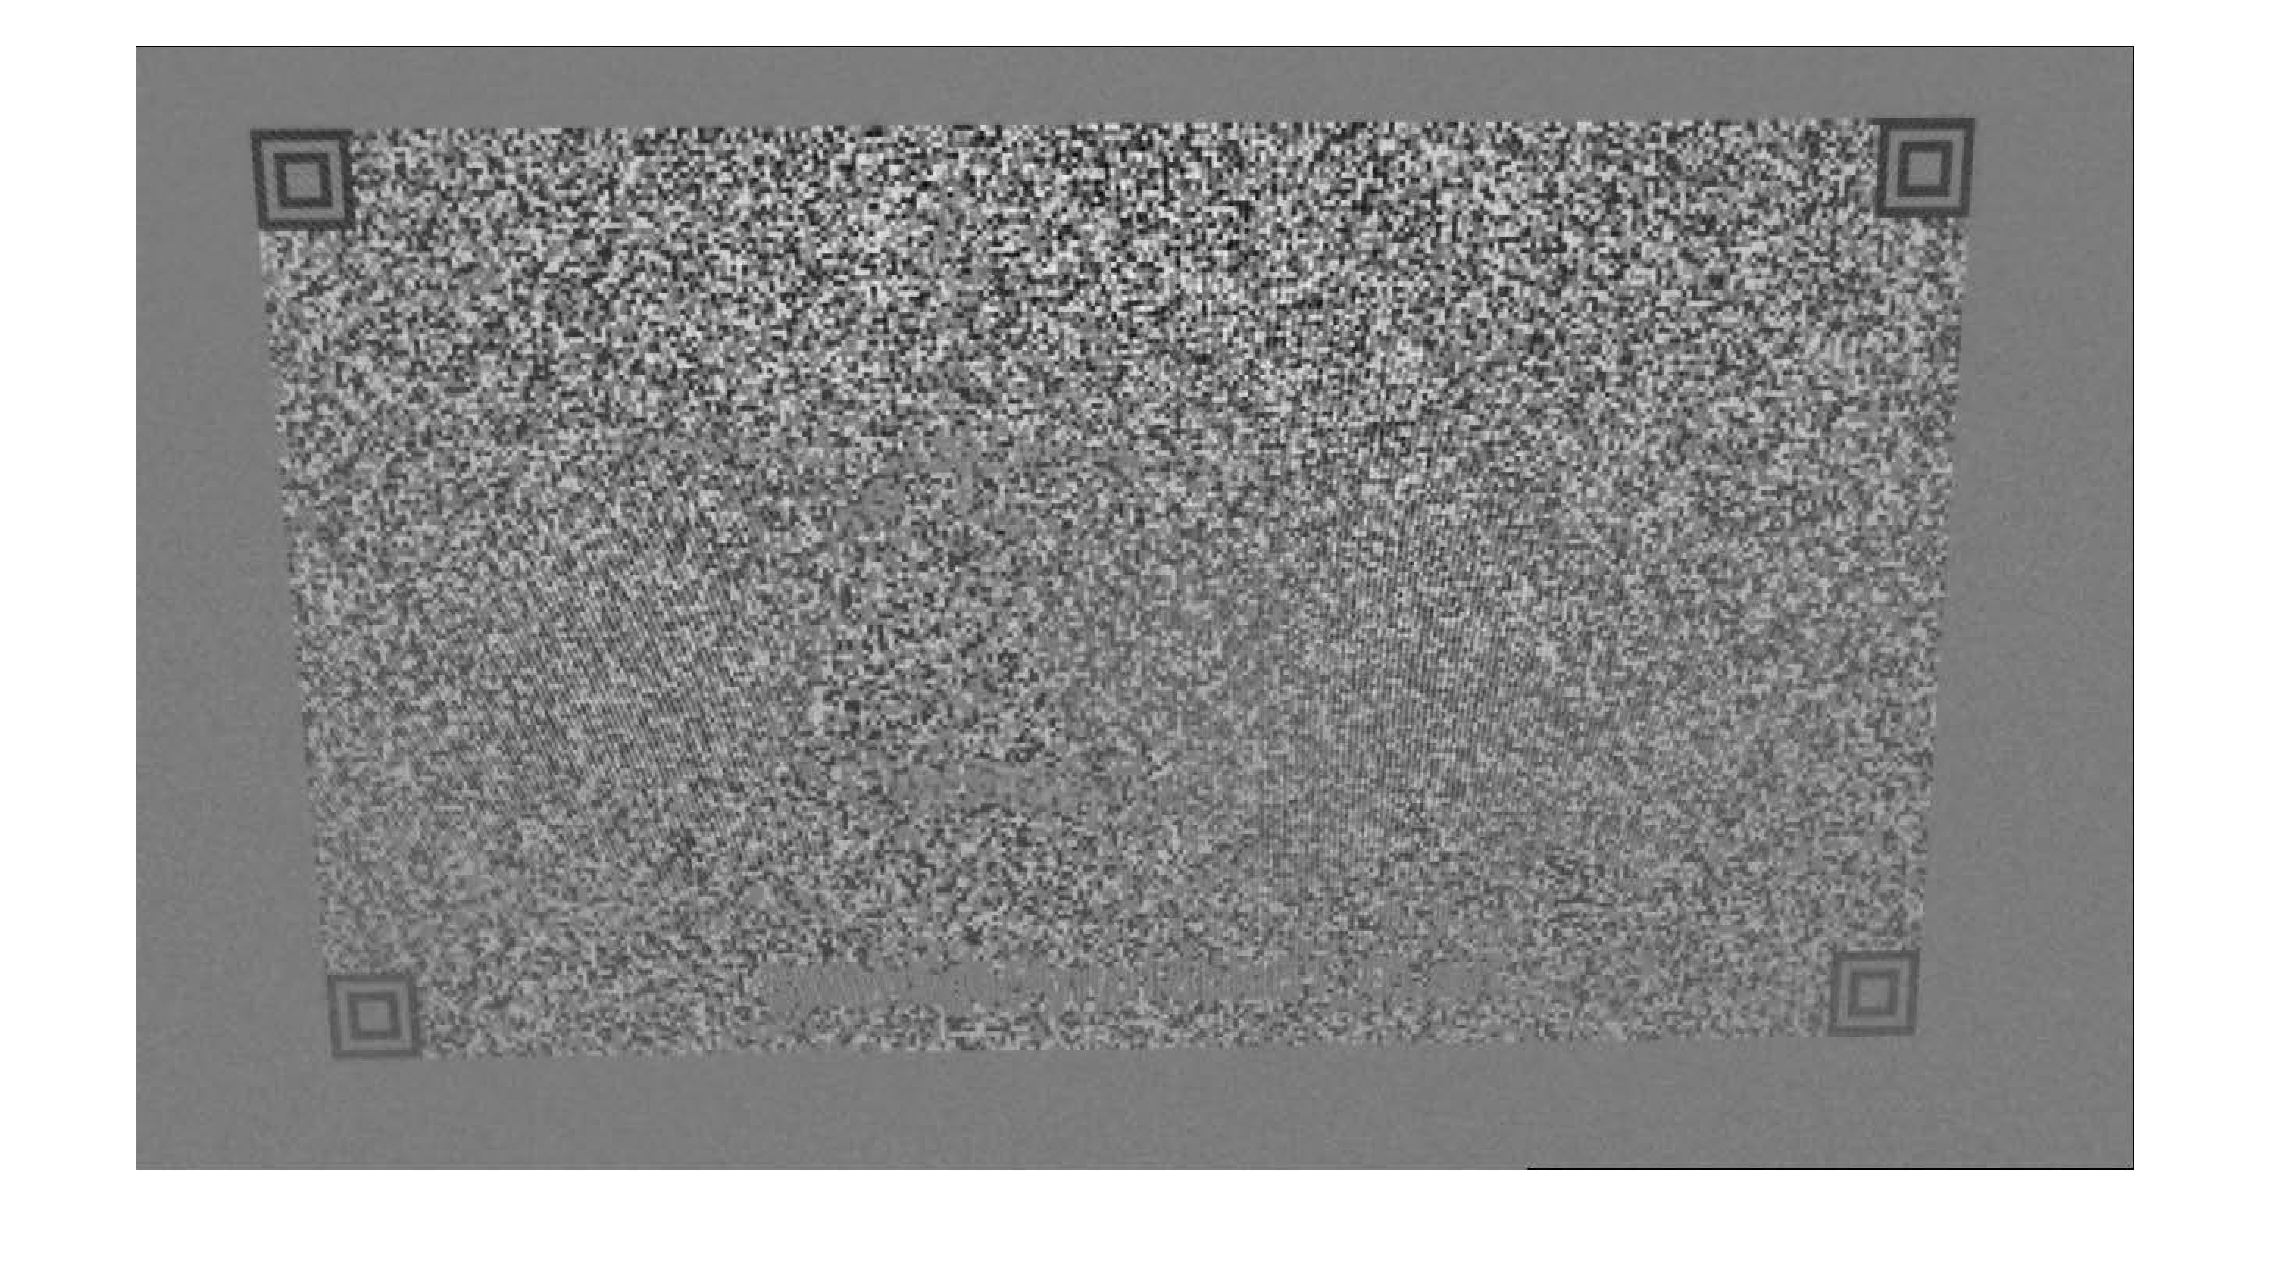
\includegraphics[scale=0.15]{images/3_Ersteverfahren/Differenzbild/2weis.pdf}& Nein & 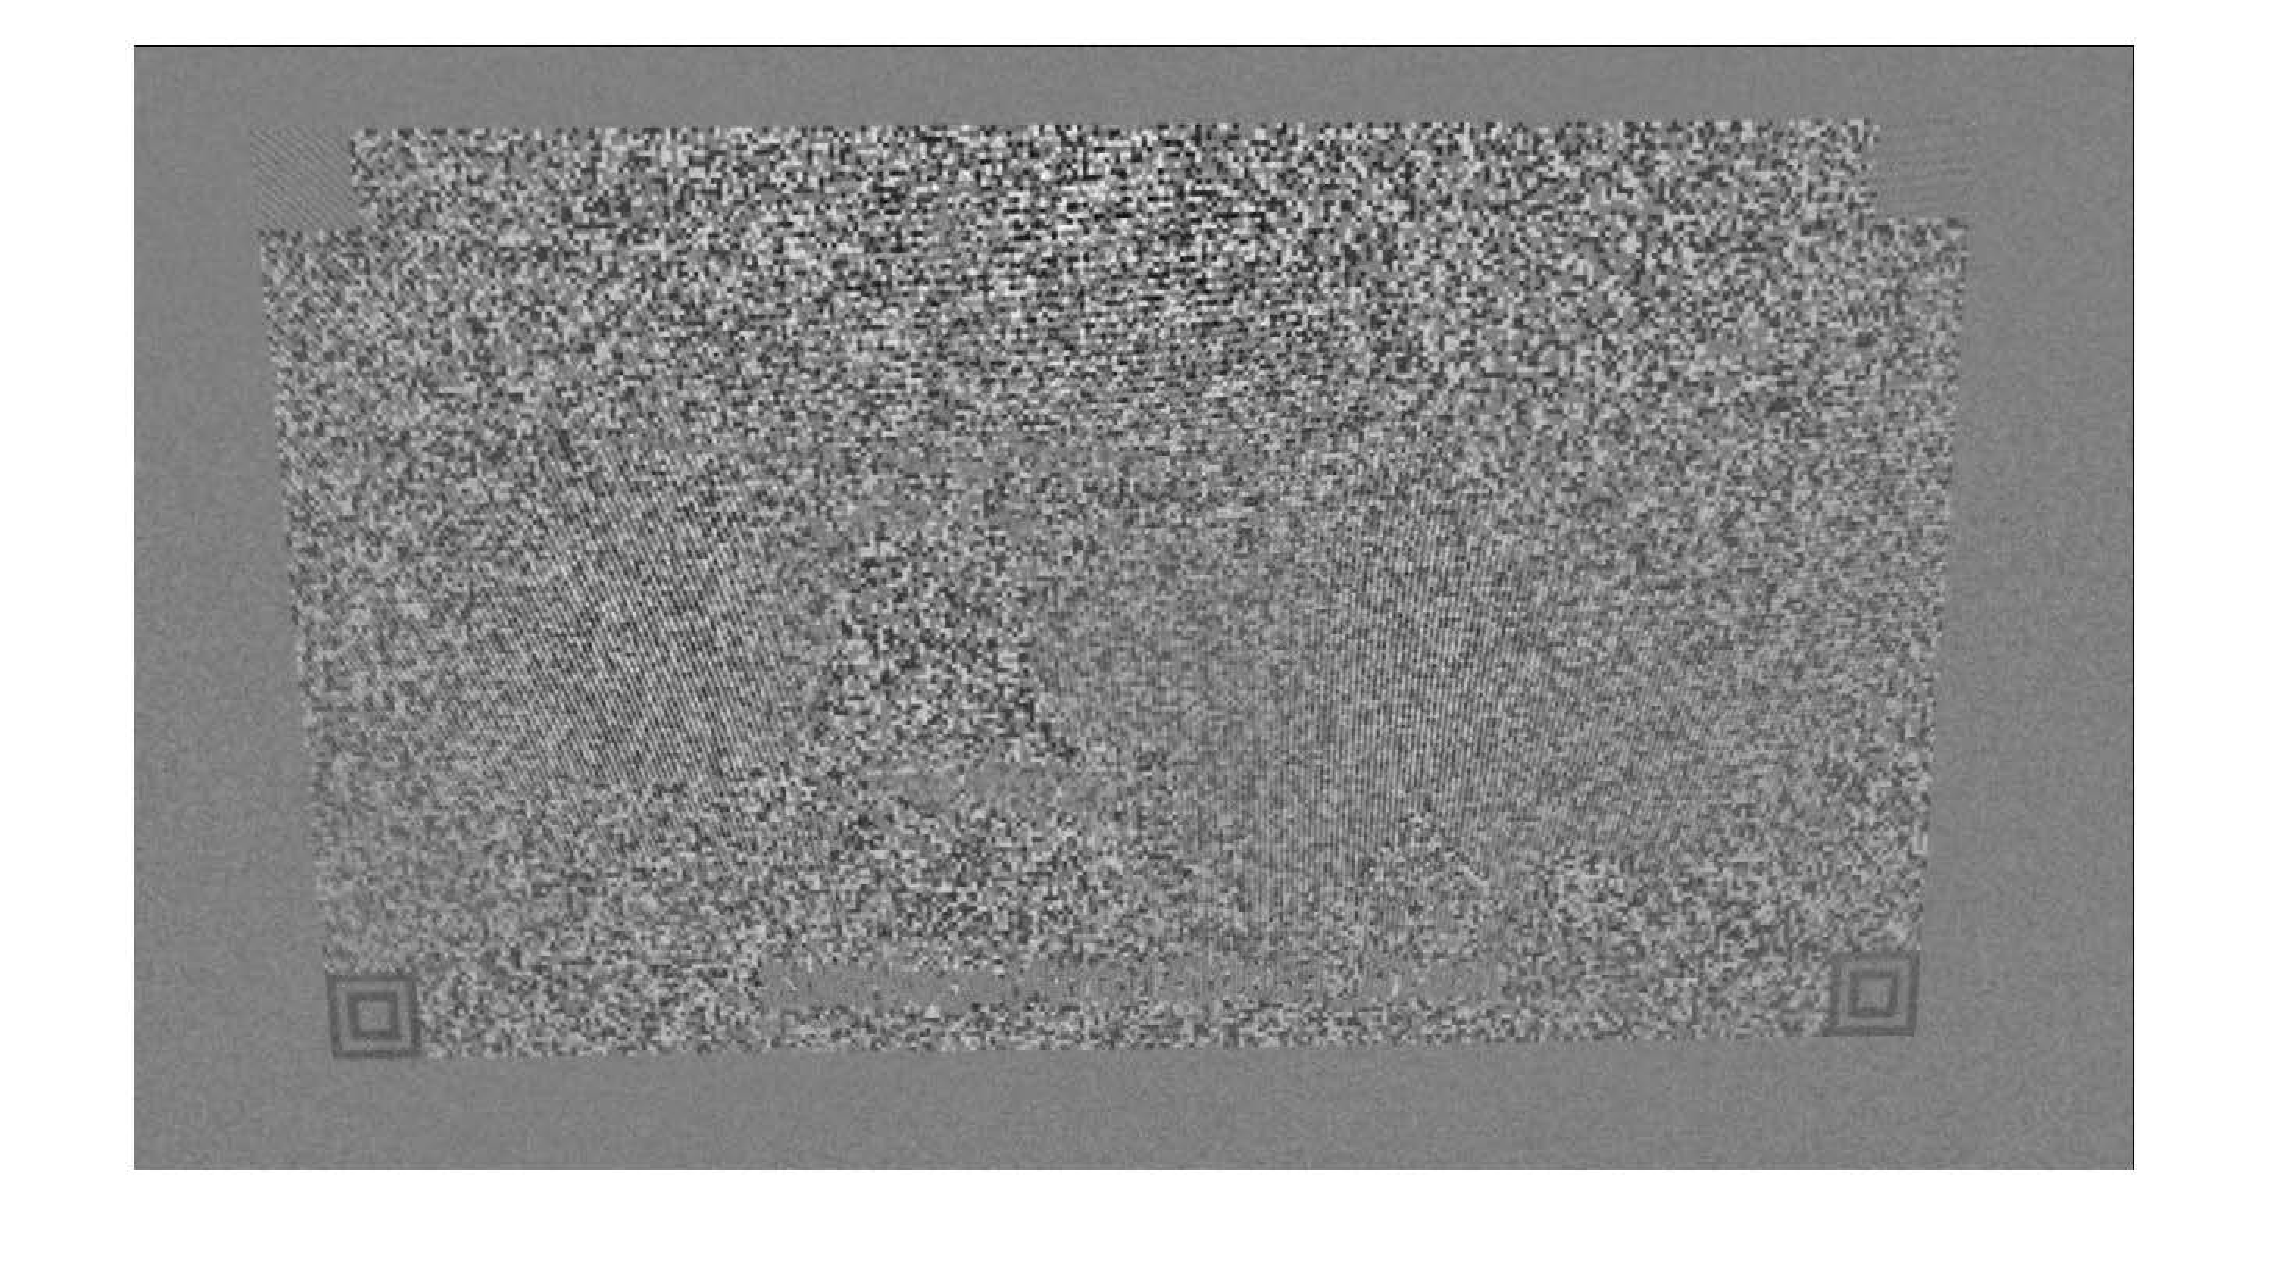
\includegraphics[scale=0.15]{images/3_Ersteverfahren/Differenzbild/3halfweis.pdf}\\
	Nein & 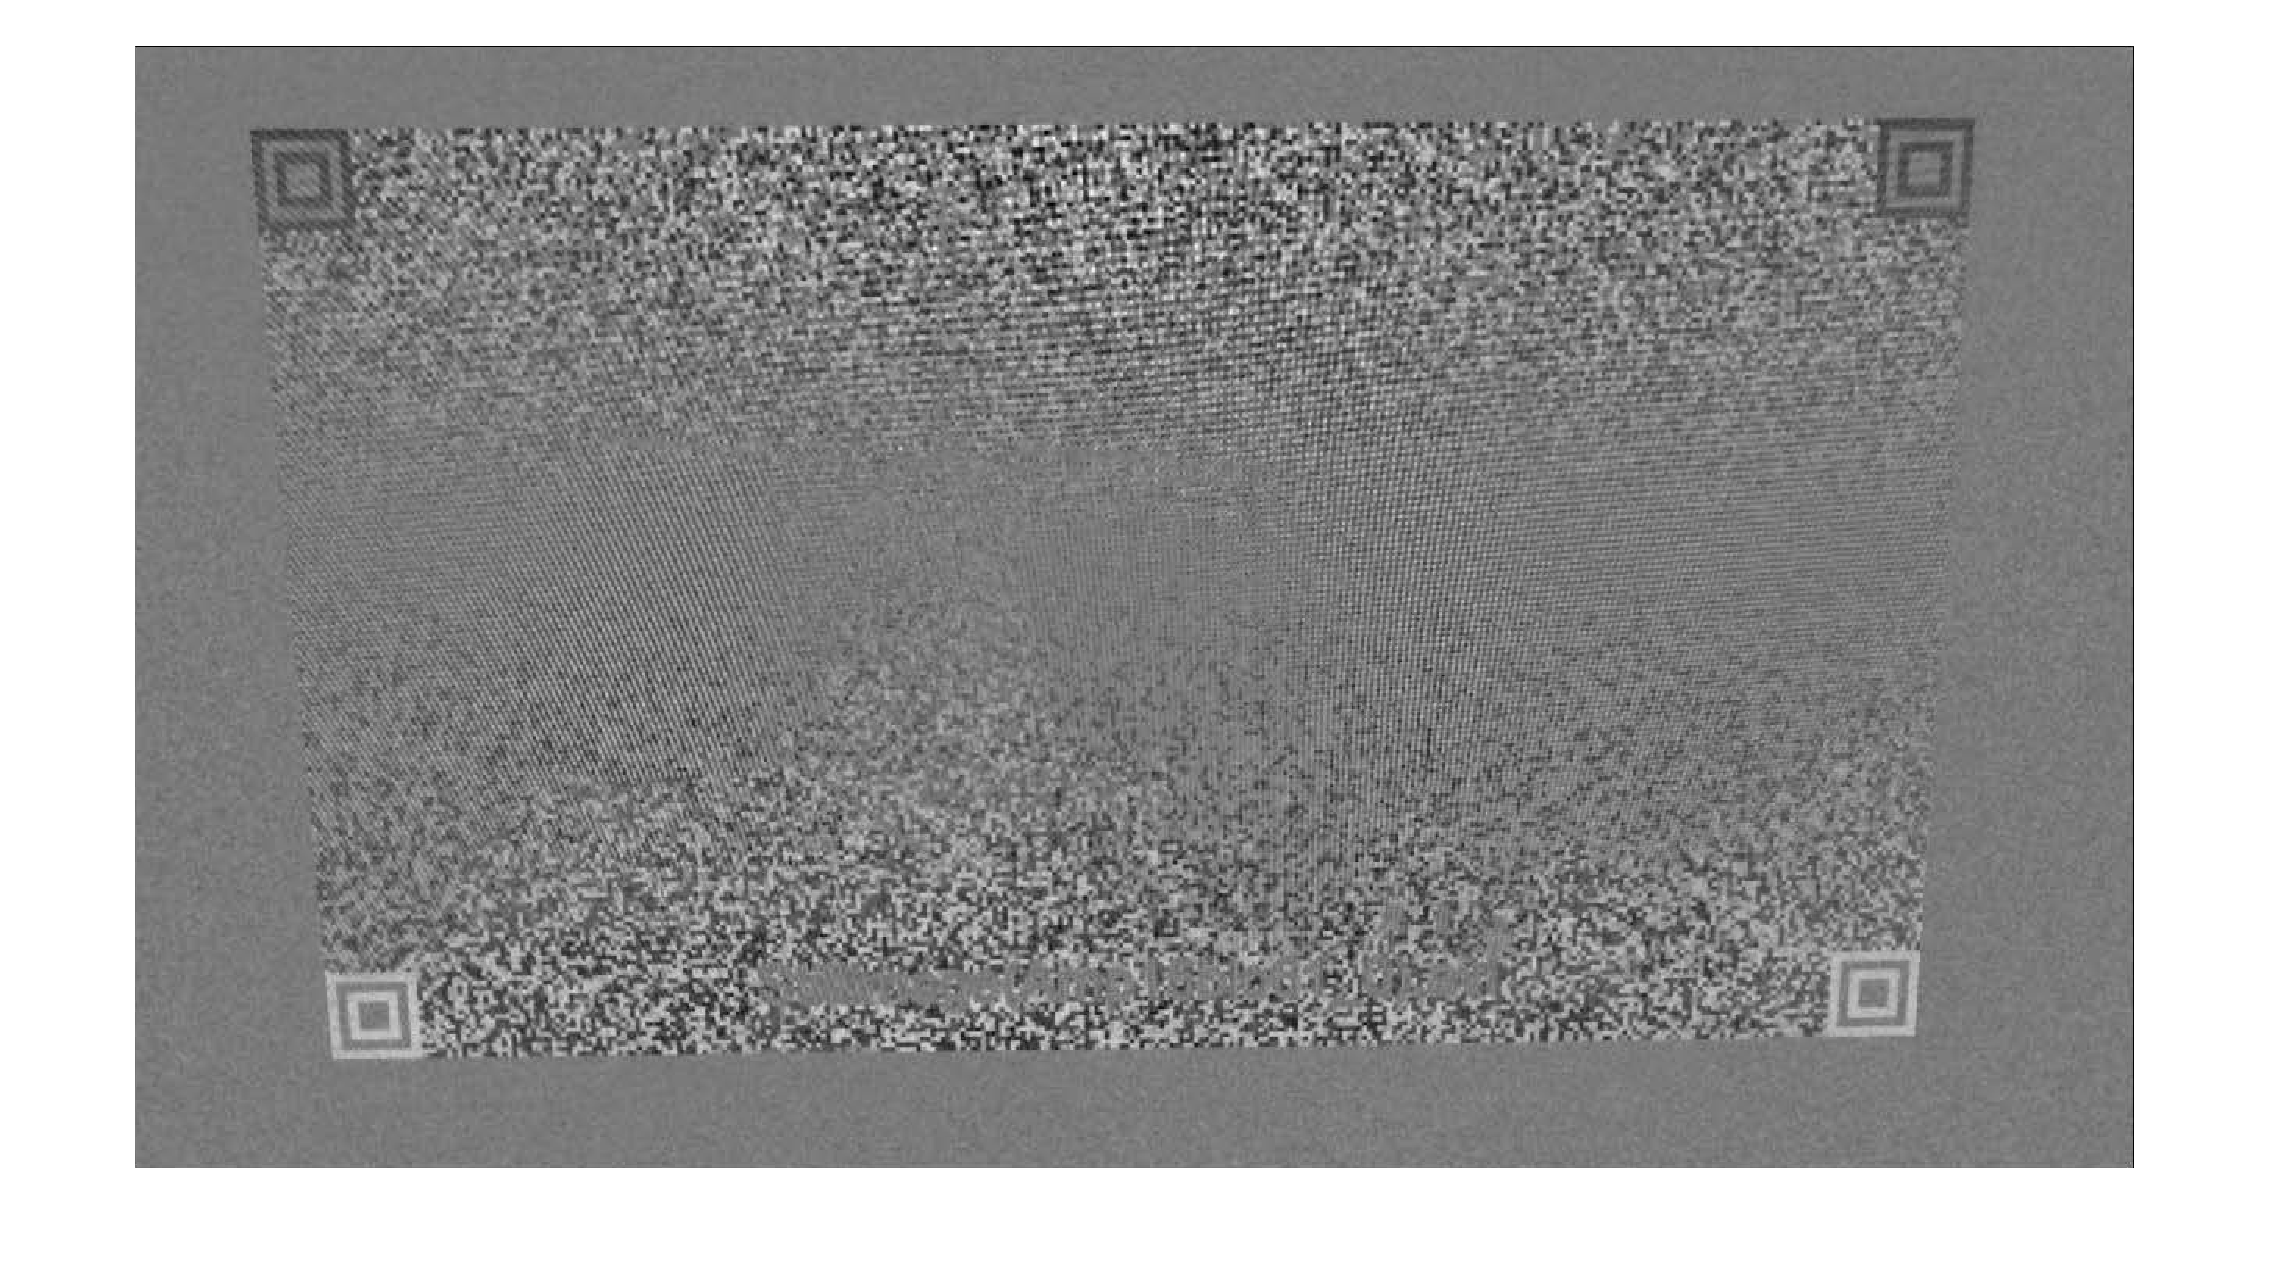
\includegraphics[scale=0.15]{images/3_Ersteverfahren/Differenzbild/4halbschwaryhalbweis.pdf}& Nein & 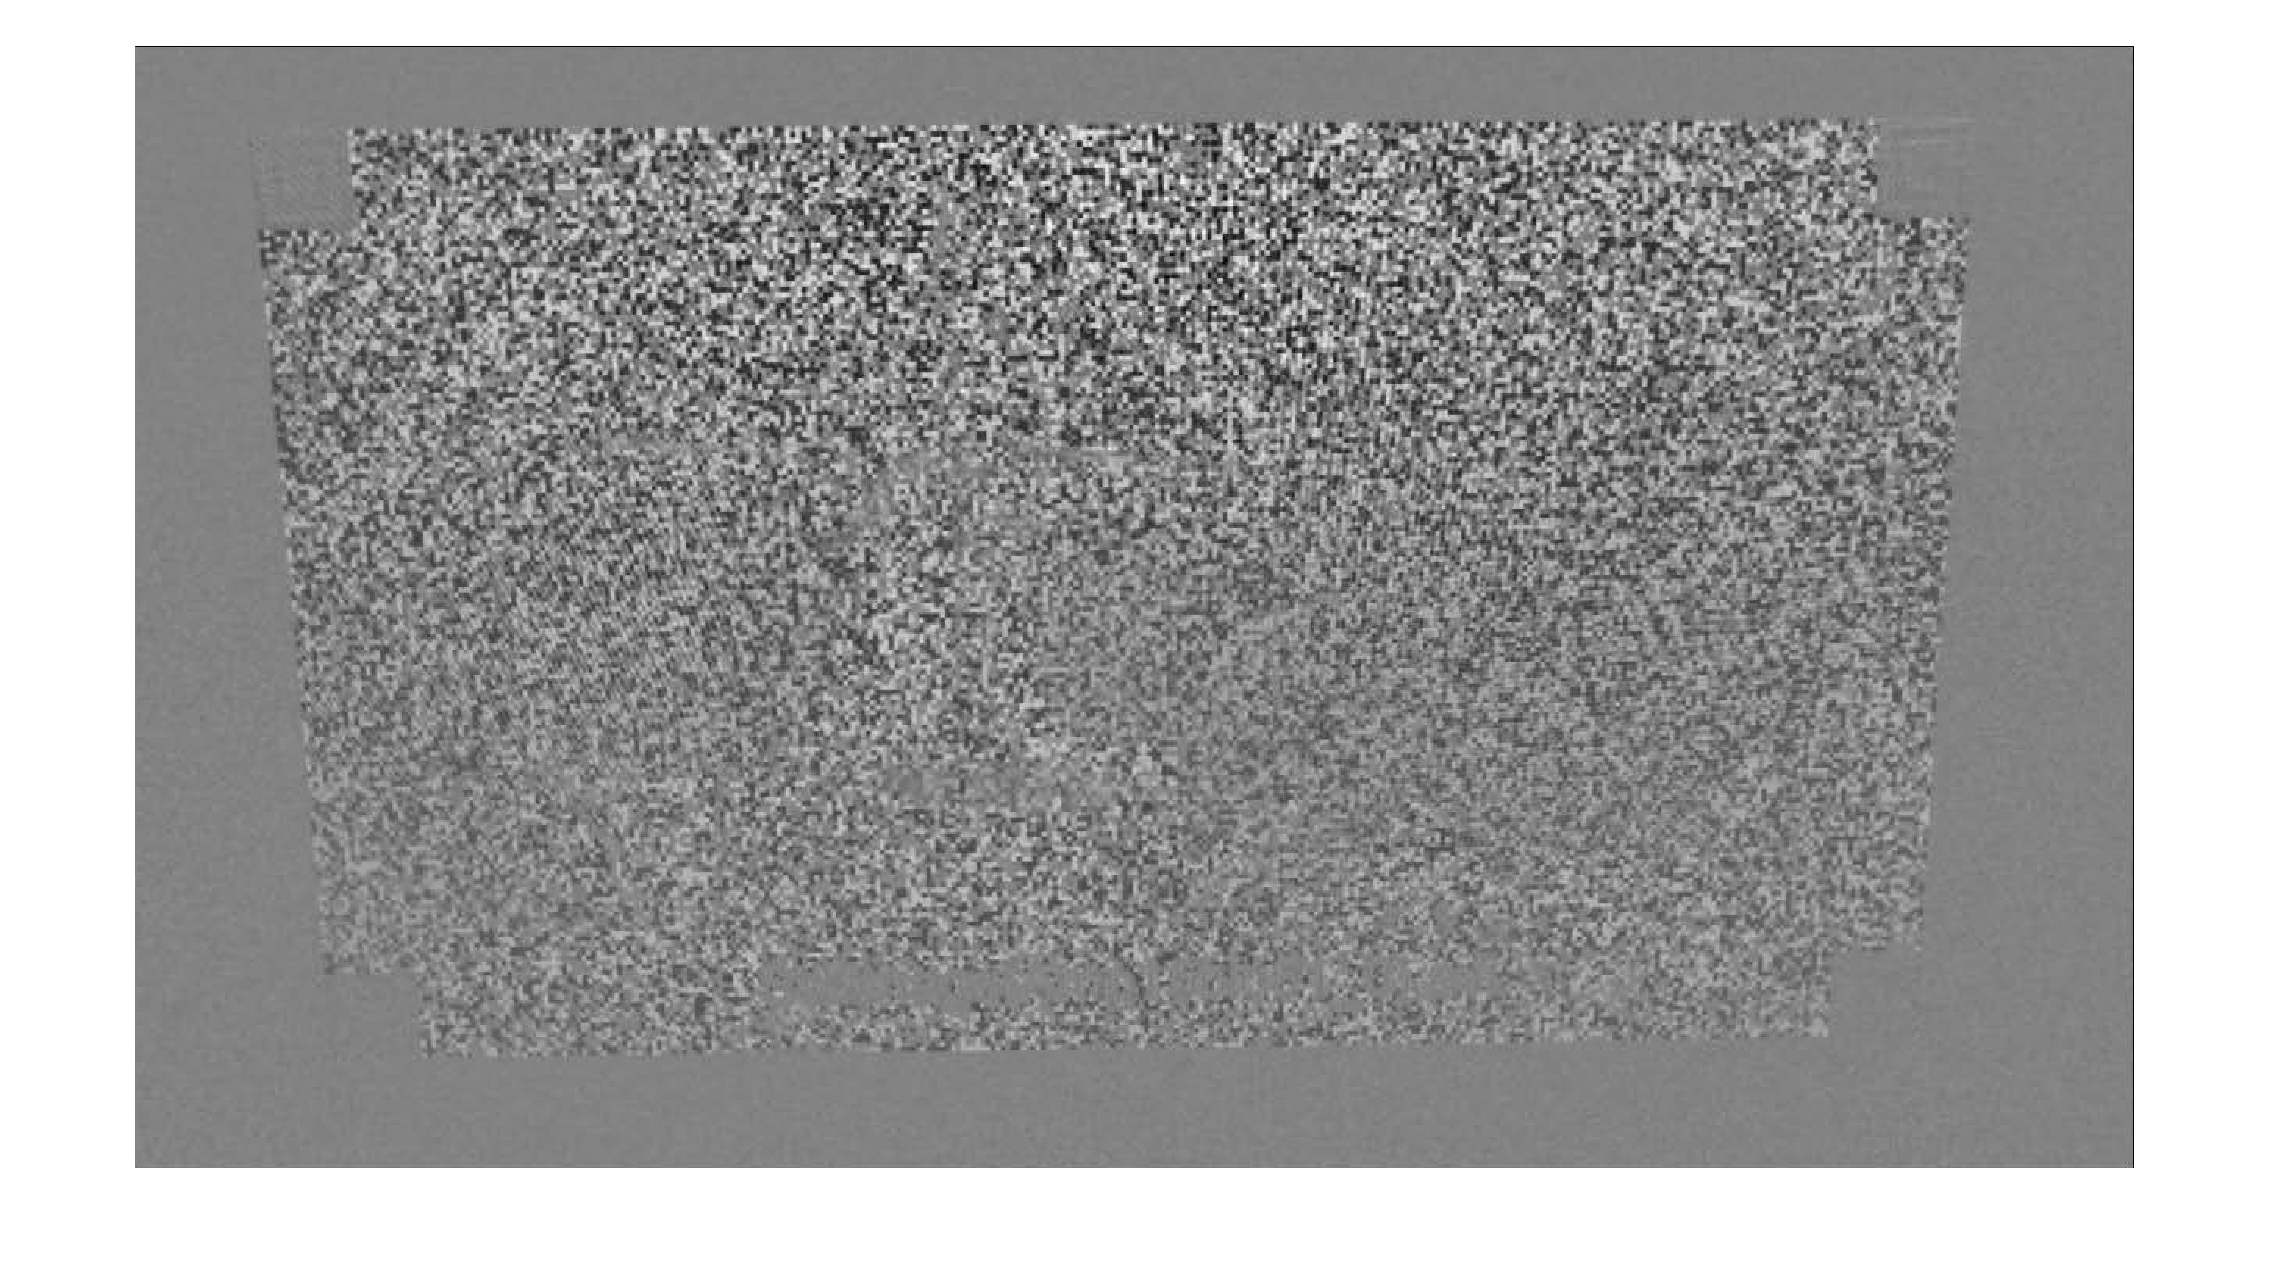
\includegraphics[scale=0.15]{images/3_Ersteverfahren/Differenzbild/5aufheben.pdf}\\

	\bottomrule
	\end{tabular}
\end{table} 


Die Struktur eines QR Musters ist in Formel 3.29 aufgeführt. Die äußerste $``1"$ Schicht ist hier ein Trennmuster und der Zentralbereich repräsentiert das QR Muster. Aufgrund der Modulationseigenschaften des \gls{david} Systems werden nur die Pixelwerte der Punkte mit dem Element $``1"$ nach der Modulation verändert. Im Vergleich dazu werden die Pixelwerte der Punkte mit dem Element $``0"$ nur gering verändert. Deswegen werden durch eine Absolutwertoperation die QR Muster als Schwarz-Weiß-Schwarz-Weiß-Schwarz Ordnung dargestellt. Dies ist die erwartete Modellstruktur die im nächsten Schritt operiert wird. Ein detailliertes Operieren wird im Abschnitt $ ``QR\,Muster\,Detektion" $ besprochen.

\begin{equation}
QR_{base} = \begin{bmatrix}
    1 &1 &1 &1 &1 &1 &1 &1 &1 \\
    1 &0 &0 &0 &0 &0 &0 &0 &1 \\
    1 &0 &1 &1 &1 &1 &1 &0 &1 \\ 
    1 &0 &1 &0 &0 &0 &1 &0 &1 \\ 
    1 &0 &1 &0 &0 &0 &1 &0 &1 \\ 
    1 &0 &1 &0 &0 &0 &1 &0 &1 \\ 
    1 &0 &1 &1 &1 &1 &1 &0 &1 \\ 
    1 &0 &0 &0 &0 &0 &0 &0 &1 \\ 
    1 &1 &1 &1 &1 &1 &1 &1 &1 \\ 
\end{bmatrix}
\end{equation}

Als nächstes wird der Begriff $``Energie"$ vorgestellt. Auf numerischer Ebene beschreibt dieser den Mittelwert des quadrierten Pixelwertes des Bildes. Es ist bekannt, dass die Pixelwerte in dem Gebiet rund um den Modulationsbereich sich durch Subtraktion der beiden Frames gegeneinander aufheben. In diesem Gebiet werden die Pixelwerte nur vom Rauschen beeinflußt und haben deshalb einen sehr kleinen Wert. Im Vergleich dazu betragen die Pixelwerte im Modulationbereich einen relativ großen Wert $\pm2A$, hier ist A die Modulationsamplitude des Systems. Der Einfluss von Zeitsynchronisation gleicht die Pixelwerte in einigen Teilen des Modulationsbereichs aufgrund von Synchronisation aus, und zwar durch aufheben der $ ``Energie" $. Die Größe der $``Energie"$ hängt hauptsächlich von den Pixelwerten im Modulationsbereich ab. Je größer die Pixelwerte sind, desto höher die $``Energie"$ des Bildes, und desto klarer kann das QR Muster werden. Gemäß dieser Regel wird die $``Energie"$ jedes Differenzbildes berechnet und in absteigender Reihenfolge angeordnet. Um die folgende Detektion zu vereinfachen, werden die ersten paar Bilder hinzugefügt. Dann wird ein zu detektierende Bilder erhaltet. %Aus dem Experiment hat bewiesen, dass es ausreicht die ersten drei Bilder zu nehmen.

Die Formel der $``Energie"$ wird in Gleichung 3.30 dargestellt. Hier repräsentiert $ m,n $ die Anzahl der Zeilen und Spalten der Matrix. $diff(i,j)$ ist der Pixelwert des Punkts in der m-ten Zeile und n-ten Spalte der Matrix.

\begin{equation}
Energie = \frac{1}{m \times n} \sum_{i=1}^m \sum_{j=1}^n diff^2(i,j) 
\end{equation}

Es folgen die detaillierten Schritte dieses Algorithmus:

\begin{enumerate}
	\item Wahl zwei beliebiger Bilder und Subtraktion dieser Bilder um das Differenzbild zu erhalten.
	\item Berechnung der Energie durch eine Absolutoperation.
	\item Sortierung in absteigender Reihenfolge und Auswahl einiger Bilder.
	\item Addition der gewählten Differenzbilder um ein zu detektierendes Bild zu erhalten.
\end{enumerate}

Dazu, das passende Flussdiagramm in Abbildung \ref{fig:DifferenzbildFlussigdiagramm}.
\begin{figure}[H]
 \centering 
 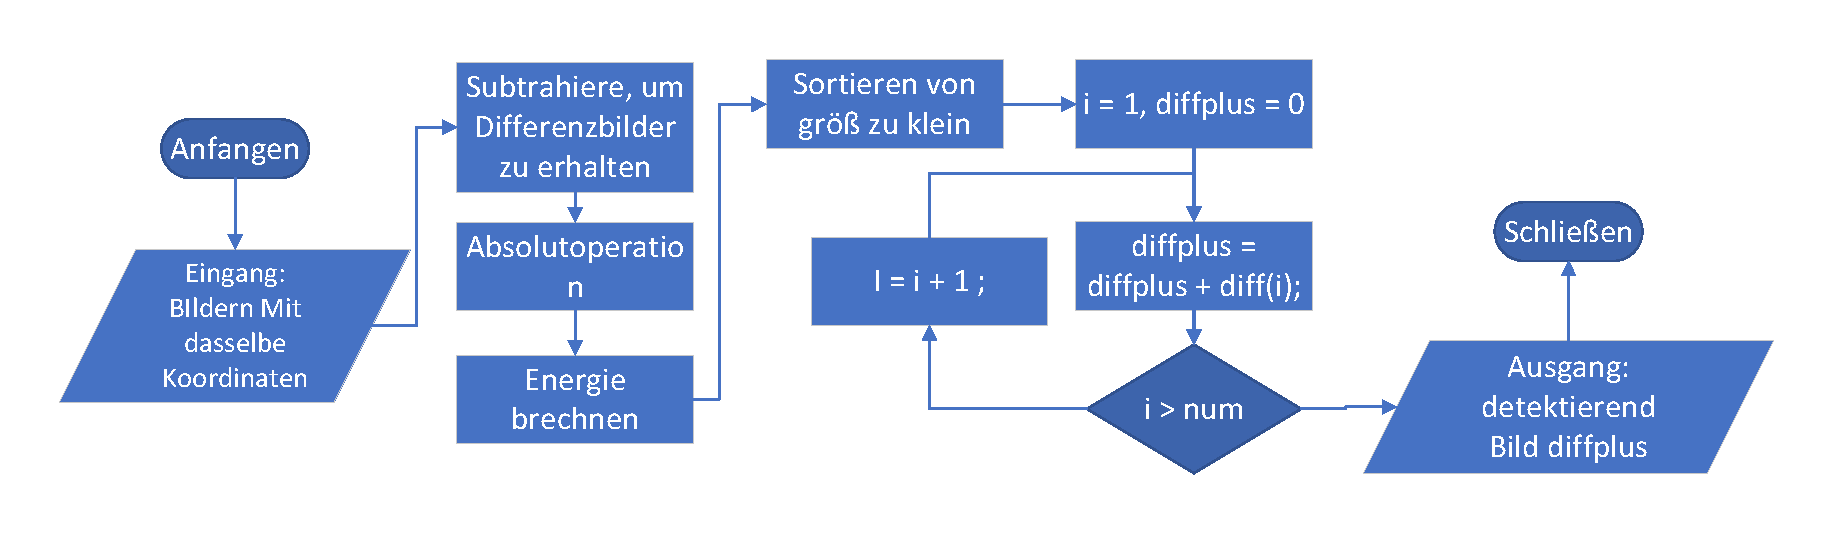
\includegraphics[keepaspectratio,width=1.1\textwidth]{images/3_Ersteverfahren/Differenzbild/Differenzbildflussigdiagramm.pdf}
 \caption{Differenzbild Flussdiagramm}
 \label{fig:DifferenzbildFlussigdiagramm}
\end{figure} 

Ein Beispiel für ein zu detektierendes Bild wird in Abbildung \ref{fig:EindetektiertesBild} vorgeführt. Aus der Abbildung ist ersichtlich, dass der Modulationsbereich besser dargestellt ist und an den vier Ecken des Bereichs ein eindeutiges QR Muster vorhanden ist. Als nächstes wird die Bildverarbeitung vorgestellt.

\begin{figure}[H]
 \centering 
 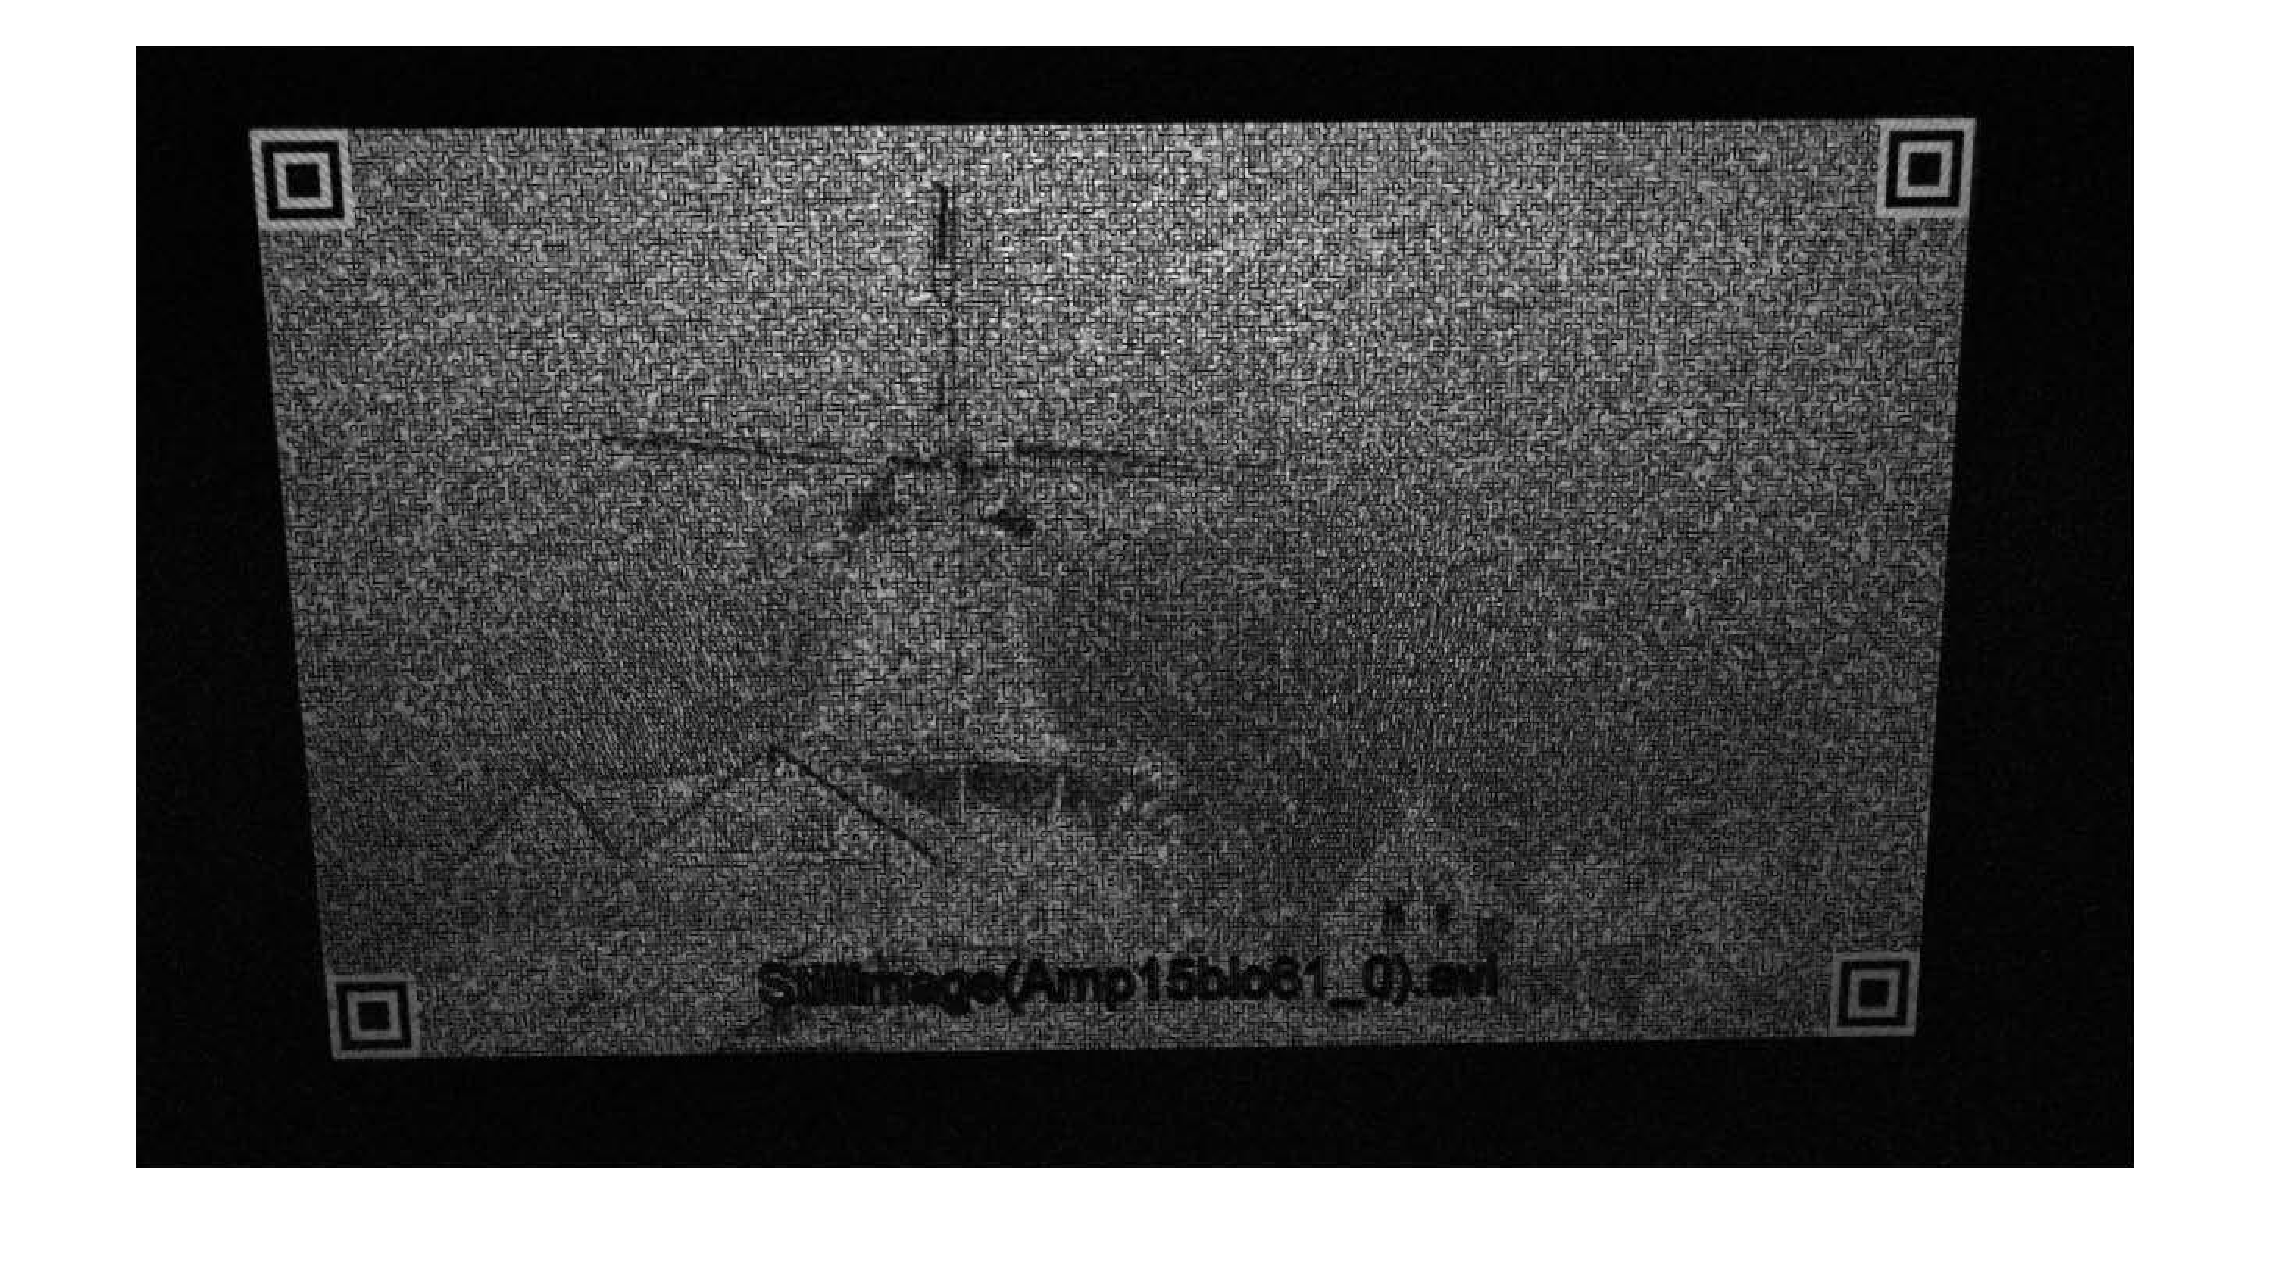
\includegraphics[keepaspectratio,width=0.8\textwidth]{images/3_Ersteverfahren/Differenzbild/diffplus.pdf}
 \caption{Ein zu detektierendes Bild}
 \label{fig:EindetektiertesBild}
\end{figure} 


\section{Bildverarbeitung} 
Durch die Differnzbild-Optimierung, wird ein zu detektierendes Bild erhalten. Abbildung \ref{fig:EindetektiertesBild} ist noch ein Graustufenbild und muss noch einiger Bildverarbeitung unterzogen werden. Dadurch können kleine Punkte und Lücken, die durch Rauschen und Fehler verursacht wurden, entfernt werden um die nachfolgende Detektion zu erleichtern. Der detaillierte Inhalt der Bildverarbeitung wurde in der anderen Methode aufgeführt. Es folgt eine kurze Beschreibung. 

\textbf{Bild Binarisierung}

Für die Schwellenwertbildung und das Erstellen eines Binärbildes wurde eine Funktion namens $ ``imbinarize" $ in Matlab verwendet. Dieser Funktion wird das Bild übergeben, damit es einen anpassungsfähigen Schwellwert generiert um das Schwarz-Weiß-Bild zu erstellen. Dies ist ausreichend für die QR Muster Detektion, weil es nur schwarze und weiße Module enthält, die binär 1 bzw. 0 sind. 

%\textbf{Medianfilter}

%Der Grund für das Median-Filtern ist, dass manchmal beim Prozess der Binarisierung aus einem Bild Effekte wie Salz- und Pfeffergeräusche entstehen können. Um diesen Fehler zu vermeiden, ist Median Filterung eine zuverlässige Methode. Eine Funktion namens $ ``medfilt2" $ wurde in Matlab verwendet. Zur Verbesserung der Ergebnisse können auch die verschiedenen Fenstergrößen für die Matlab-Funktion verwendet werden.

\textbf{Morphologie}

Mit öffnenden und schließenden Filtern können die Lücken zwischen Blöcken und die Punkte vom Rauschen stark reduziert werden, was das binär Bild zu einer guten Interpretation des QR Musters macht. 

\section{QR Muster Detektion} 

Nach der Bildverarbeitung wird nun die QR Muster Detektion ausgeführt. Das Ziel einer QR Muster Detektion ist, das Zentrum des Musters im Bild zu lokalisieren um dadurch das Bild zu rekonstruieren. Abbildung \ref{fig:QRPattern} zeigt die geometrische Struktur eines QR Musters. An jeder Ecke des Modulartionsbereichs gibt es ein solches QR Muster.

\begin{figure}[H]
 \centering 
 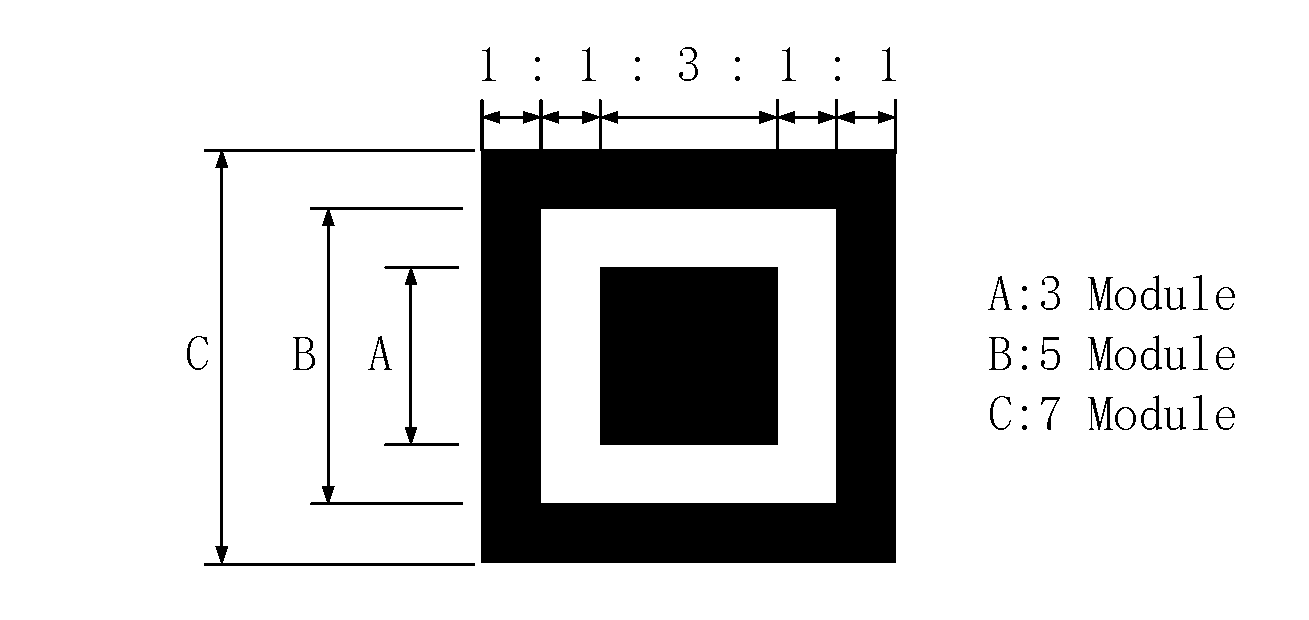
\includegraphics[keepaspectratio,width=0.9\textwidth]{images/3_Ersteverfahren/QRMuster/QRPattern.pdf}
 \caption{QR Muster}
 \label{fig:QRPattern}
\end{figure}

Aus der geometrischen Sicht kann jedes Muster als drei konzentrische Quadrate betrachtet werden und besteht aus einem schwarzen (dunklen) $7 \times 7$ Modul, einem weißen (hellen) $5 \times 5$ Modul und schließlich einem schwarzen (dunklen) $3 \times 3$ Modul. Von Kenntnissen der Geometrie ist bekannt, dass in jeder Richtung das Breiteverhältnis der alternativen Schwarz- und Weißmodul in einem Muster die Beziehung $1:1:3:1:1$ existiert, wie es in Abbildung \ref{fig:QRPatternRatio} vorgeführt ist. Diese wichtige Eigenschaft hilft uns, die Positionen der QR Muster zu finden. In der Praxis gibt es rund um die Muster noch ein Trennmuster, das ein Funktionsmuster aller weißen (hellen) Module (ein Modul breit) ist. Es dient als eine Grenze zwischen den Mustern und dem Datenbereich, um die Verwechslung zwischen Muster und Daten zu vermeiden.
 
 \begin{figure}[H]
 \centering 
 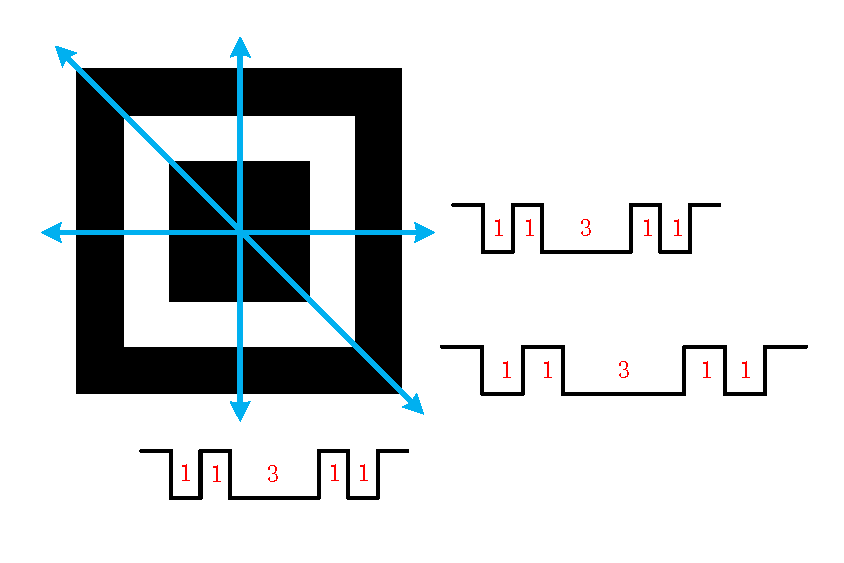
\includegraphics[keepaspectratio,width=0.7\textwidth]{images/3_Ersteverfahren/QRMuster/QP_Patternratio.pdf}
 \caption{QR Muster Ratio}
 \label{fig:QRPatternRatio}
\end{figure}

Als nächstes werden die detaillierten Schritte der Detektion aufgeführt welche mit der Funktion $ ``detectFIP" $ in Matlab implementiert wurde.

\textbf{Schritt 1:}

Zuerst wird der Berechnungsaufwand der Analyse des ganzen Bildes geschätzt, und anschließend wird der Modulationsbereich in kleine Bereiche unterteilt, die die QR Muster beinhalten.

\textbf{Schritt 2:}

Scannen jeder Zeile dieses kleinen Bereiches und Speicherung der Länge der Schwarz und Weiß Module in einen fünf Elementen Vektor. Die Länge der Module bedeutet die Anzahl aufeinanderfolgender Pixel in einer Zeile mit der gleichen Farbe. Die Speicherreihenfolge in diesem Vektor ist Schwarz-Weiß-Schwarz-Weiß-Schwarz. Es sollte hier angemerkt werden, dass das erste Element des Vektors die Anzahl der schwarzen Module enthält. 

\textbf{Schritt 3:}

Immer wenn das fünfte Element des Vektors gezählt wird, werden die Werte ausgewertet, ob das Muster nahe genug an den $1:1:3:1:1$ Verhältnissen daran ist. Wenn die Bedingung erfüllt ist, gehen zum Schritt 4. Ansonsten wird der Vektor um zwei Elemente nach links verschoben und die ersten zwei Elemente des Vektors werden entfernt. Kehren zum Schritt 2 zurück.
              

\textbf{Schritt 4:}

Die Elemente vom Vektor werden verarbeitet, um das ungefähre horizontale Zentrum zu erhalten. Eine Kreuzprüfung wird an diesem Punkt vorgenommen, welche aus den Schritten 2 und 3 besteht, der Unterschied besteht darin, dass der horizontale Scan durch einen vertikalen Scan ersetzt wird. Anschließend wird überprüft, ob ein vertikales Zentrum gefunden wurde. Wenn Ja wird eine Kreuz-Kreuzprüfung mit dem horizontalen Scan vorgenommen, um die Ergebnisse zu optimieren. Dies wird hauptsächlich benötigt, um die reale horizontale Mitte des Musters in extremen Schräglage Fällen zu lokalisieren. Nach Speicherung des potenziellen Zentrums, werden die Elemente des Vektors geleert um wieder im zweiten Schritt einen Scan zu machen. Ansonsten wird der Vektor um zwei nach links verschoben und die ersten beiden Elemente des Vektors weggeworfen. In Schritt 2, wird wiederum erneut begonnen zu scannen und zu zählen.  

\textbf{Schritt 5:}

Die Ausgabe des vorherigen Schritts wird verarbeitet. Falls mehrere potentielle Muster gefunden wurden, wird $ ``Select Best Pattern" $ verwendet, um das Beste Auszuwählen. Es sollte angemerkt werden, dass wenn die möglichen Muster nach dem Ende der Erkundung nicht gefunden wurden, ein spezielles Signal zurückgegeben wird und das System zur Schritt Differenzbild Optimierung zurückkehren wird. Die Operation besteht darin dem ursprünglichen Bild, welches aus einige Differenzbildern besteht, ein mehreres Differenzbild hinzuzufügen.
                       
\textbf{Schritt 6:}

Durch die gefundenen Muster Zentren, wird eine projektive Transformation vorgenommen, um die Ecken des Bildes zu bestimmen.


Die folgende Abbildung \ref{fig:FlussdiagrammQRMuster} zeigt ein Flussdiagramm einer Detektion für QR Muster.

\begin{figure}[htb]
 \centering 
 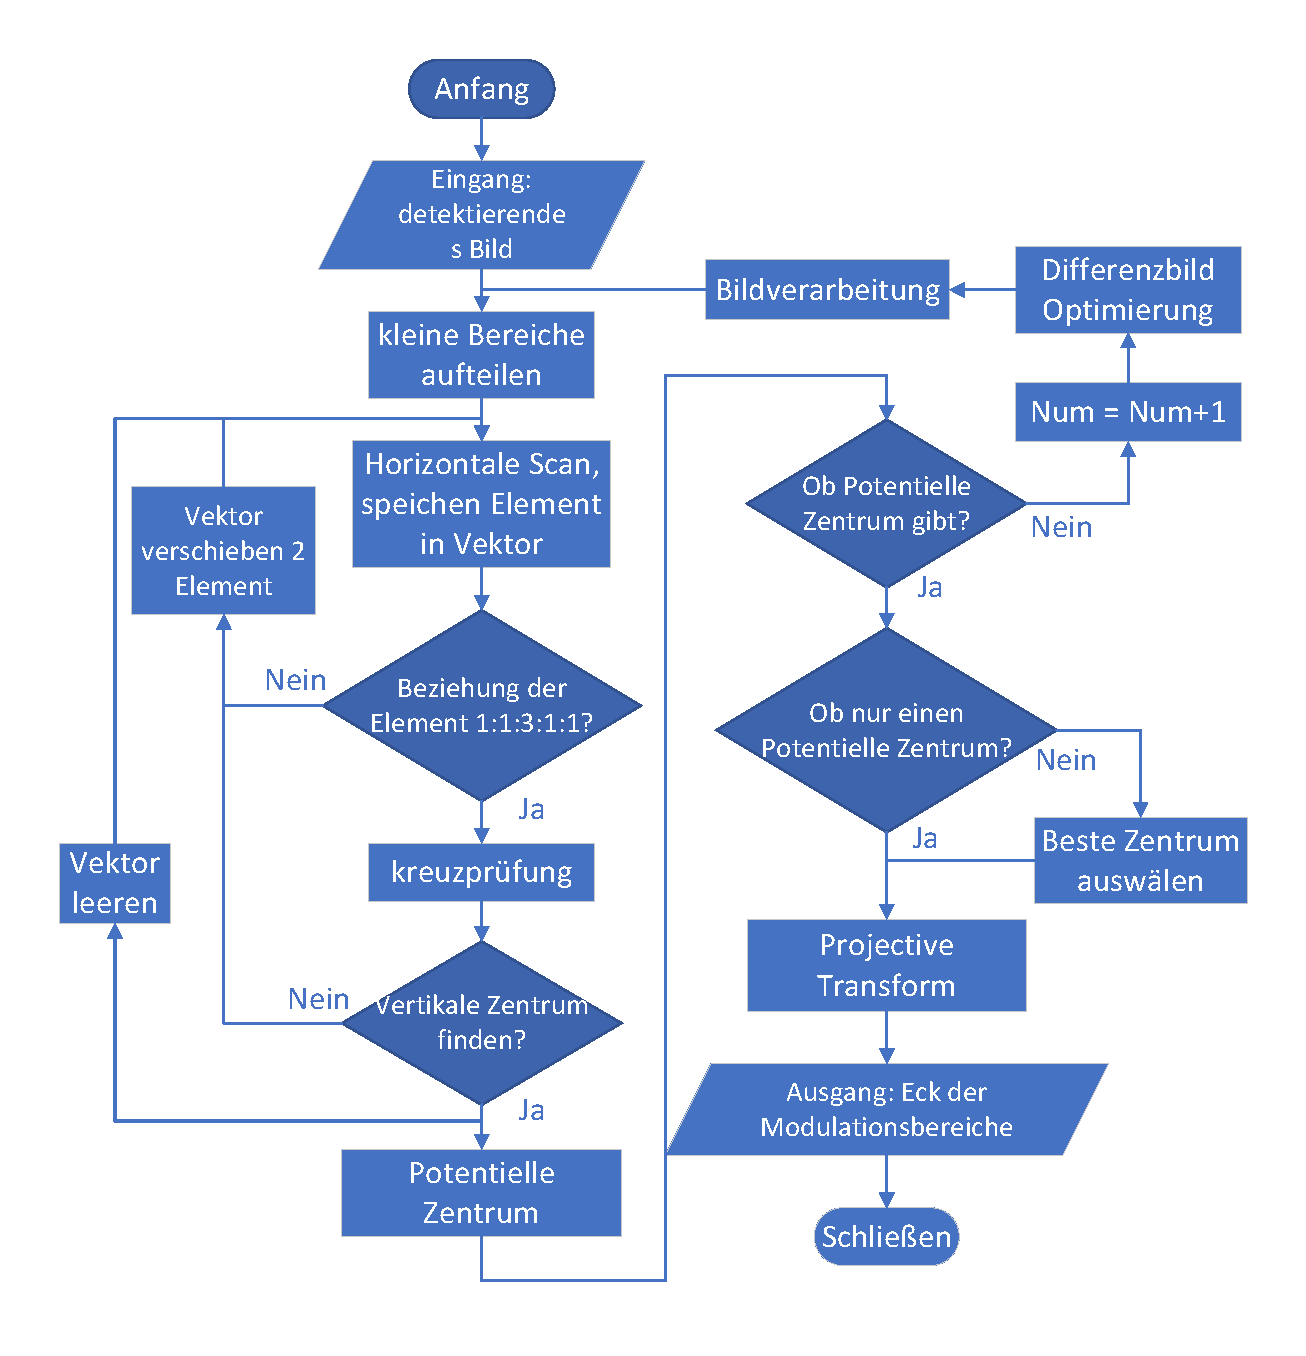
\includegraphics[keepaspectratio,width=1.0\textwidth]{images/3_Ersteverfahren/QRMuster/QR_flussdiagramm.pdf}
 \caption{Flussdiagramm der QR Muster Detektion}
 \label{fig:FlussdiagrammQRMuster}
\end{figure}

Ein Beipiel für QR Muster Detektion wird in Abbildung \ref{fig:QRMusterBeispiel} vorgeführt:

\begin{figure}[htb]
 \centering 
 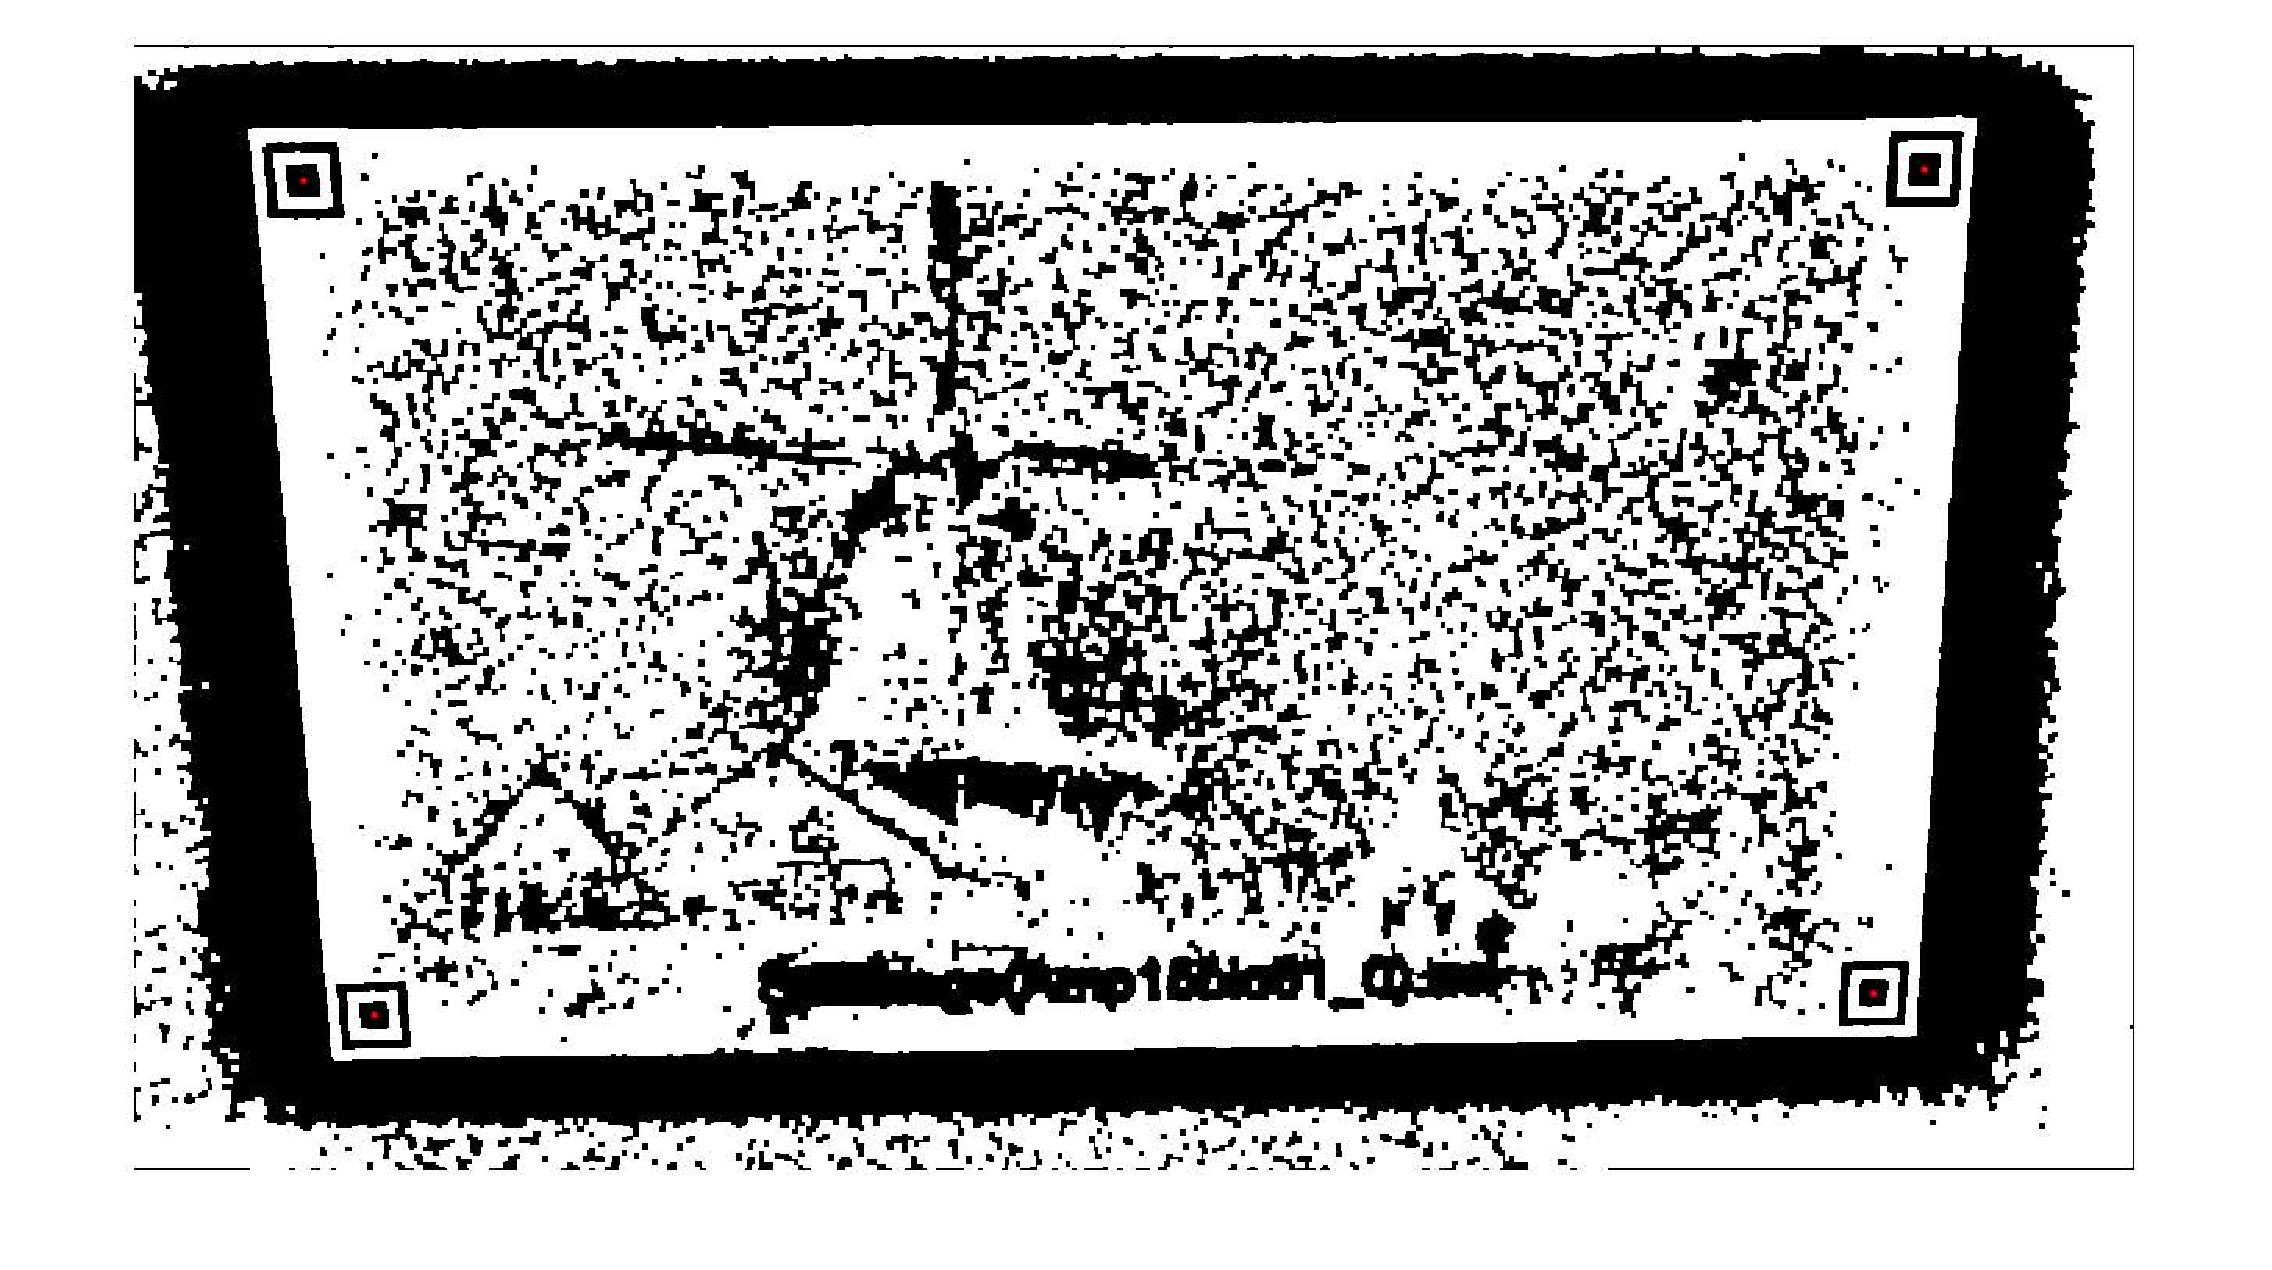
\includegraphics[keepaspectratio,width=1.0\textwidth]{images/3_Ersteverfahren/QRMuster/QR_Patterndetektion.pdf}
 \caption{Beispiel einer QR Muster Detektion}
 \label{fig:QRMusterBeispiel}
\end{figure}